\documentclass[11pt,a4paper]{article}
\usepackage{isabelle,isabellesym, amsmath}
\usepackage{times}
\usepackage{graphicx}
\usepackage{amssymb}

\normalfont
\setlength\parindent{24pt}
\newcommand{\isactrlemph}[1]{\emph{#1}}
\usepackage{setspace}
\doublespacing



% further packages required for unusual symbols (see also
% isabellesym.sty), use only when needed

\usepackage{amssymb}
  %for \<leadsto>, \<box>, \<diamond>, \<sqsupset>, \<mho>, \<Join>,
  %\<lhd>, \<lesssim>, \<greatersim>, \<lessapprox>, \<greaterapprox>,
  %\<triangleq>, \<yen>, \<lozenge>

%\usepackage{eurosym}
  %for \<euro>

%\usepackage[only,bigsqcap]{stmaryrd}
  %for \<Sqinter>

%\usepackage{eufrak}
  %for \<AA> ... \<ZZ>, \<aa> ... \<zz> (also included in amssymb)

%\usepackage{textcomp}
  %for \<onequarter>, \<onehalf>, \<threequarters>, \<degree>, \<cent>,
  %\<currency>

% this should be the last package used
\usepackage{pdfsetup}

% urls in roman style, theory text in math-similar italics
\urlstyle{rm}
\isabellestyle{it}

% for uniform font size
%\renewcommand{\isastyle}{\isastyleminor}


\begin{document}

\title{Three Implementations of the Categorical Imperative}
\author{Lavanya Singh}
\maketitle

\tableofcontents

\newpage

% sane default for proof documents
\parindent 0pt\parskip 0.5ex

% generated text of all theories
%
\begin{isabellebody}%
\setisabellecontext{paper}%
%
\isadelimtheory
%
\endisadelimtheory
%
\isatagtheory
%
\endisatagtheory
{\isafoldtheory}%
%
\isadelimtheory
%
\endisadelimtheory
%
\isadelimdocument
%
\endisadelimdocument
%
\isatagdocument
%
\isamarkupsection{Introduction%
}
\isamarkuptrue%
%
\endisatagdocument
{\isafolddocument}%
%
\isadelimdocument
%
\endisadelimdocument
%
\begin{isamarkuptext}%
As artifical reasoners become increasingly powerful, computers become increasingly able to 
perform complex ethical reasoning. The field of machine ethics \cite{mesurvey} is attractive for two reasons.
First, the proliferation of artifically autonomous agents is creating and will continue to create a demand for 
ethical autonomous agents. These agents must be able to model and reason about complex ethical theories 
that withstand philosophical scrutiny. Second, just as automated mathematical reasoning gives mathematicians
new powers and proof-finding ability, automated ethical reasoning is a tool that philosophers can use 
when reasoning about ethics. Many contradictions or paradoxes with an ethical system may not be 
immediately obvious to the human eye, but can be easily tested using an automated theorem prover.

Modelling ethics without sacrificing the intracacies and complexities of an ethical theory is a 
challenging computational and philosophical problem. Simple and intuitive computational approaches, 
such as encoding ethical rules as constraints in a constraint satisfaction problem, fail to capture
the complexity of most philosophically plausible systems. On the other hand, it is not immediately clear
how to formalize many complex moral theories, like virtue ethics.

Computational ethics also requires a sophisticated 
ethical theory to model. Constraint satisfaction systems often default to some version of utiliarianism, 
the principle of doing the most good for the most people. Alternatively, they model basic moral 
principles such as ``do not kill," without modelling the theory that these principles originated from.
Modelling a more complex ethical theory will not only enable smarter philosophical machines, it will
also empower philosophers to study more complex ethical issues with the computer's help. The entire
field of philosophy is devoted to developing and testing robust ethical theories. Plausible machine
ethics must draw on plausible moral philosophy.

The ideal candidate ethical theory will be both philosophically interesting and easy to 
formalize. Kantian ethics, often described as ``formal," has been often floated as such a candidate \cite{powers, BL}. 
The categorical imperative, Kant's universal law of morality, is a moral rule that can be used to 
guide action. 

This project's objective is to automate reasoning about Kantian ethics. I present two different
formalizations of Kant's categorical imperative implemented and tested in the Isabelle/HOL \cite{isabelle} theorem prover.
Each formalization is modelled as an extension of Carmo and Jones' Dyadic Deontic Logic (DDL). The corresponding 
DDL formalization is then embedded in higher-order logic (HOL) and implemented in Isabelle. Section 
3.1 implements and tests the naive formalization, a control group that is equivalent to DDL 
itself. Section 3.2 examines a more sophisticated formalization inspired by Moshe Kroy's partial 
formalization of thecategorical imperative. 

I contribute implementations of two different interpretations of the categorical imperative, 
examples of how each implementation can be used to model and solve ethical scenarios, and tests that
examine ethical and logical properties of the system, including logical consistency, consistency
of obligation, and possibility of permissibility. The implementations themselves are usable models 
of ethical principles and the tests represent the kind of philosophical work that formalized ethics 
can contribute.%
\end{isamarkuptext}\isamarkuptrue%
%
\isadelimdocument
%
\endisadelimdocument
%
\isatagdocument
%
\isamarkupsection{System Overview \label{sec:overview}%
}
\isamarkuptrue%
%
\endisatagdocument
{\isafolddocument}%
%
\isadelimdocument
%
\endisadelimdocument
%
\begin{isamarkuptext}%
The goal of this project is to automate sophisticated ethical reasoning. This requires three
components. First, the choice of an ethical theory that is both intuitively attractive and 
lends itself to formalization. Second, the choice of formal logic to model the theory in. Third, the 
choice of automation engine to implement the formal model in. Section 2.1 introduces Kantian
ethics, Section 2.2 explains Carmo and Jones's Dyadic Deontic Logic \cite{CJDDL} as a 
base logic, and Section 2.3 presents the Isabelle/HOL implementation of the logic.%
\end{isamarkuptext}\isamarkuptrue%
%
\isadelimdocument
%
\endisadelimdocument
%
\isatagdocument
%
\isamarkupsubsection{Kantian Ethics \label{sec:kant}%
}
\isamarkuptrue%
%
\endisatagdocument
{\isafolddocument}%
%
\isadelimdocument
%
\endisadelimdocument
%
\begin{isamarkuptext}%
Kantian ethics is an attractive choice of ethical theory to automate for two reasons. The 
first is that Kant's writings have been a major inspiration for much of Western analytic philosophy. 
In addition to the rich neo-Kantian program, almost all major philosophical traditions after Kant have
engaged with his work. Much of Western libertarian political thought is inspired by Kant's deontology,
and his ethics have bled into household ethical thought. Deontology is seen as one of the three major 
schools of Western normative philosophy.

Understanding the ethic's potential for formalization requires understanding Kant's system. Kant argues 
that if morality exists, it must take the form of an inviolable rule, which he calls the ``categorical
imperative." He presents three formulations of the categorical imperative, as well as a robust defense
of them in his seminal work on ethics \cite{groundwork}. He argues that all three formulations are 
equivalent. 

The first formulation of the categorical imperative is the ``Formula of Universal Law." 

$\textbf{Definition}$ \emph{(Formula of Universal Law)}

\emph{I ought never to act except in such a way that I could also will that my maxim should become a universal law} \cite{groundwork}

A ``maxim" is roughly a moral rule like ``I can murder someone to take their job". ``Willing" a maxim is 
equivalent to acting on that rule. The FUL creates a thought experiment called the universalizability 
test: to decide if a maxim is permissible, imagine what would happen if everyone willed that maxim. 
If your imagined world yields a contradiction, the maxim is prohibited\footnote{There is another case here.
What happens if the imagined world does not yield a logical contradiction, but is still undesirable? Kant 
distinguishes between these cases as contradictions in conception and contradictions in will. Both yield moral
prohibitions, but contradictions in conception generate stronger contradictions and therefore stronger obligations. 
This paper will focus entirely on contradictions in conception, for this is the only kind of contradiction 
for which a strict logical interpretation makes sense. For a complete treatment of the difference, see \cite{groundwork, KorsgaardFUL}}. Intuitively, the FUL asks 
the question, "What would happen if everyone did that?" \cite{KorsgaardFUL}. 

As an example, let's apply the universalizability test to the maxim of murdering others to take their job.
Universalized, anyone who wants a job can murder the person currently holding that job. It is contradictory
to simultaneously will that I acquire a job (through murder) and also that someone can take that job from me 
whenever they want (also by murder). The maxim thwarts its own end, and is thus internally contradictory.
 Therefore, this maxim is prohibited.

The universalizability test makes the ``formal" nature of Kant's ethics immediately clear. Formal 
logic has the tools to universalize a maxim (apply a universal quantifier) and to test for 
contradictions (test for inconsistency). 

Kant also presents two additional formulations of the categorical imperative. 

$\textbf{Definition}$ \emph{(Formula of Humanity)}

\emph{The Formula of Humanity (FUH)
is to act in such a way "that you use humanity, whether in your own person or in the person
of any other, always at the same time as an end, never merely as a means."}\cite{groundwork}

\medskip 

$\textbf{Definition}$ \emph{(Kingdom of Ends)}

\emph{The third formulation of the categorical imperative states that "we should so act that we may 
think of ourselves as legislating universal laws through our maxims."}\cite{KorsgaardFUL}

The last two formulations are not as obviously formal as the FUL, but they can still be
modelled in logic. Because Kantian ethics presents a series of rules, a logical system can encode 
the theory by modelling each rule as an axiom.

The above outline is a brief and incomplete picture of a rich philosophical tradition. Kantian scholars
debate the meaning of each formulation of the categorical imperative and develop views far more 
nuanced than those above. For the purposes of this paper, I will adopt Kant's three original 
formulations presented above. Note additionally that Kantian ethics is widely disputed. I do not present 
a defense of Kant's ethic in this paper. My approach to formalizing ethics can be applied to other 
theories as well.  

This paper aims to formalize Kant's ethic as faithfully as possible. This is an important choice. 
While it is tempting to modify or simplify an ethical theory in seemingly insignificant way, these 
choices often have ramifications. The entire field of neo-Kantian thought 
has been exploring versions of Kant's ethical theory for centuries. I will not attempt to present a 
radically new conception of Kant's ethic, but will instead draw on philosophical expertise regarding
the content and justification of the categorical imperative.%
\end{isamarkuptext}\isamarkuptrue%
%
\isadelimdocument
%
\endisadelimdocument
%
\isatagdocument
%
\isamarkupsubsection{Dyadic Deontic Logic%
}
\isamarkuptrue%
%
\isamarkupsubsubsection{Deontic Logic%
}
\isamarkuptrue%
%
\endisatagdocument
{\isafolddocument}%
%
\isadelimdocument
%
\endisadelimdocument
%
\begin{isamarkuptext}%
Traditional modal logics include $\Box$ operators to represent necessity. In simple modal logics like S5 \cite{cresswell} 
using the Kripke semantics, $\Box p$ is true at a world $w$ if $p$ is true at all of $w$'s neighbors. 
These logics also usually contain the $\diamond$ operator, representing possibility, where
 $\diamond p \iff \sim \Box \sim p$. Additionally, modal logics support operators of propositional 
logic like $\sim, \wedge, \vee, \rightarrow$.

A deontic logic is a special kind of modal logic designed to reason about obligation. Standard deontic
logic \cite{cresswell, sep-logic-deontic} essentially replaces $\Box$ with the obligation operator
$O$, and $\diamond$ with the permissibility operator $P$. Using the Kripke semantics for $O$, $O p$ 
is true at $w$ if $p$ is true at all  ideal deontic alternatives to $w$. The $O$ operator in SDL
takes a single argument (the formula that is obligatory), and is thus called a monadic deontic operator.

 While SDL is appreciable for its simplicity, it suffers a variety of well-documented paradoxes, 
including contrary-to-duty paradoxes \footnote{The paradigm case of a contrary-to-duty paradox is the 
Chisholm paradox. Consider the following statements: \begin{enumerate}
\item It ought to be that Tom ought helps his neighbors
\item It ought to be that if Tom goes to help his neighbors, he tells them he is coming
\item If Tom does not go to help his neighbors, he ought not tell them that he is coming
\item Tom does not help his neighbors
\end{enumerate} 
These premises contradict themselves, because items (2)-(4) imply that Tom ought not help his neighbors. The 
contradiction results because the logic cannot handle violations of duty mixed with
conditionals. \cite{chisholm, ctd}
}. 
In situations where duty is violated, the logic breaks down 
and produces paradoxical results. Thus, I use an improved deontic logic instead of SDL for this work.%
\end{isamarkuptext}\isamarkuptrue%
%
\isadelimdocument
%
\endisadelimdocument
%
\isatagdocument
%
\isamarkupsubsubsection{Dyadic Deontic Logic%
}
\isamarkuptrue%
%
\endisatagdocument
{\isafolddocument}%
%
\isadelimdocument
%
\endisadelimdocument
%
\begin{isamarkuptext}%
I use as my base logic Carmo and Jones's dyadic deontic logic, or DDL, which improves on SDL \cite{CJDDL}. 
It introduces a dyadic obligation operator $O\{A \vert B\}$ 
to represent the sentence ``A is obligated in the context B". This gracefully handles contrary-to-duty
conditionals. The obligation operator uses a neighborhood semantics \cite{neighborhood1, neighborhood2}, instead of the Kripke semantics. 
Carmo and Jones define a function $ob$ that maps from worlds to sets of sets of worlds. Intuitively, 
each world is mapped to the set of propositions obligated at that world, where a proposition $p$ is defined as 
the worlds at which the $p$ is true.

DDL also includes many other modal operators. In addition to $\Box$ and $\diamond$, DDL also has a notion
of actual obligation and possible obligation, represented by operators $O_a$ and $O_p$ respectively. 
These notions are accompanied by the corresponding modal operators $\Box_a, \diamond_a, \Box_p, \diamond_p$. 
These operators use a Kripke semantics, with the functions $av$ and $pv$ mapping a world $w$ to the set 
of corresponding actual or possible versions of $w$. 

For more of fine-grained properties of DDL see \cite{CJDDL} or this project's source code. DDL is quite a heavy logic and contains many modal operators 
that aren't necessary for my analysis. While this expressivity is powerful, it may also cause performance
impacts. In particular, DDL has a large set of axioms involving quantification over complex higher-order
logical expressions. Proofs involving these axioms will be computationally expensive.  Benzmueller 
and Parent warned me that this may become a problem if Isabelle's automated proof tools begin to time out.%
\end{isamarkuptext}\isamarkuptrue%
%
\isadelimdocument
%
\endisadelimdocument
%
\isatagdocument
%
\endisatagdocument
{\isafolddocument}%
%
\isadelimdocument
%
\endisadelimdocument
%
\isadelimtheory
%
\endisadelimtheory
%
\isatagtheory
%
\endisatagtheory
{\isafoldtheory}%
%
\isadelimtheory
%
\endisadelimtheory
%
\end{isabellebody}%
\endinput
%:%file=~/Desktop/cs91r/paper/paper.thy%:%
%:%24=6%:%
%:%36=8%:%
%:%37=9%:%
%:%38=10%:%
%:%39=11%:%
%:%40=12%:%
%:%41=13%:%
%:%42=14%:%
%:%43=15%:%
%:%44=16%:%
%:%45=17%:%
%:%46=18%:%
%:%47=19%:%
%:%48=20%:%
%:%49=21%:%
%:%50=22%:%
%:%51=23%:%
%:%52=24%:%
%:%53=25%:%
%:%54=26%:%
%:%55=27%:%
%:%56=28%:%
%:%57=29%:%
%:%58=30%:%
%:%59=31%:%
%:%60=32%:%
%:%61=33%:%
%:%62=34%:%
%:%63=35%:%
%:%64=36%:%
%:%65=37%:%
%:%66=38%:%
%:%67=39%:%
%:%68=40%:%
%:%69=41%:%
%:%70=42%:%
%:%71=43%:%
%:%72=44%:%
%:%73=45%:%
%:%74=46%:%
%:%75=47%:%
%:%76=48%:%
%:%77=49%:%
%:%78=50%:%
%:%87=52%:%
%:%99=54%:%
%:%100=55%:%
%:%101=56%:%
%:%102=57%:%
%:%103=58%:%
%:%104=59%:%
%:%113=61%:%
%:%125=63%:%
%:%126=64%:%
%:%127=65%:%
%:%128=66%:%
%:%129=67%:%
%:%130=68%:%
%:%131=69%:%
%:%132=70%:%
%:%133=71%:%
%:%134=72%:%
%:%135=73%:%
%:%136=74%:%
%:%137=75%:%
%:%138=76%:%
%:%139=77%:%
%:%140=78%:%
%:%141=79%:%
%:%142=80%:%
%:%143=81%:%
%:%144=82%:%
%:%145=83%:%
%:%146=84%:%
%:%147=85%:%
%:%148=86%:%
%:%149=87%:%
%:%150=88%:%
%:%151=89%:%
%:%152=90%:%
%:%153=91%:%
%:%154=92%:%
%:%155=93%:%
%:%156=94%:%
%:%157=95%:%
%:%158=96%:%
%:%159=97%:%
%:%160=98%:%
%:%161=99%:%
%:%162=100%:%
%:%163=101%:%
%:%164=102%:%
%:%165=103%:%
%:%166=104%:%
%:%167=105%:%
%:%168=106%:%
%:%169=107%:%
%:%170=108%:%
%:%171=109%:%
%:%172=110%:%
%:%173=111%:%
%:%174=112%:%
%:%175=113%:%
%:%176=114%:%
%:%177=115%:%
%:%178=116%:%
%:%179=117%:%
%:%180=118%:%
%:%181=119%:%
%:%182=120%:%
%:%183=121%:%
%:%184=122%:%
%:%185=123%:%
%:%186=124%:%
%:%187=125%:%
%:%188=126%:%
%:%189=127%:%
%:%190=128%:%
%:%191=129%:%
%:%192=130%:%
%:%193=131%:%
%:%194=132%:%
%:%195=133%:%
%:%196=134%:%
%:%205=138%:%
%:%209=140%:%
%:%221=142%:%
%:%222=143%:%
%:%223=144%:%
%:%224=145%:%
%:%225=146%:%
%:%226=147%:%
%:%227=148%:%
%:%228=149%:%
%:%229=150%:%
%:%230=151%:%
%:%231=152%:%
%:%232=153%:%
%:%233=154%:%
%:%234=155%:%
%:%235=156%:%
%:%236=157%:%
%:%237=158%:%
%:%238=159%:%
%:%239=160%:%
%:%240=161%:%
%:%241=162%:%
%:%242=163%:%
%:%243=164%:%
%:%244=165%:%
%:%245=166%:%
%:%246=167%:%
%:%255=169%:%
%:%267=171%:%
%:%268=172%:%
%:%269=173%:%
%:%270=174%:%
%:%271=175%:%
%:%272=176%:%
%:%273=177%:%
%:%274=178%:%
%:%275=179%:%
%:%276=180%:%
%:%277=181%:%
%:%278=182%:%
%:%279=183%:%
%:%280=184%:%
%:%281=185%:%
%:%282=186%:%
%:%283=187%:%
%:%284=188%:%
%:%285=189%:%
%
\begin{isabellebody}%
\setisabellecontext{paper{\isadigit{2}}{\isadigit{2}}}%
%
\isadelimtheory
%
\endisadelimtheory
%
\isatagtheory
%
\endisatagtheory
{\isafoldtheory}%
%
\isadelimtheory
%
\endisadelimtheory
%
\isadelimdocument
%
\endisadelimdocument
%
\isatagdocument
%
\isamarkupsubsection{Isabelle/HOL Implementation \label{sec:isabelle}%
}
\isamarkuptrue%
%
\endisatagdocument
{\isafolddocument}%
%
\isadelimdocument
%
\endisadelimdocument
%
\begin{isamarkuptext}%
Isabelle/HOL is an interactive proof assistant \cite{isabelle} built on Haskell and Scala. It 
allows the user to define types, functions, definitions, and axiom systems. It has built-in support for both
automatic and interactive/manual theorem proving. 

I started my project by reimplementing Benzmueller, Farjami, and Parent's \cite{BFP, logikey} implementation 
of DDL in Isabelle/HOL. This helped me learn how to use Isabelle/HOL, and the implementation showcased in the 
next few sections demonstrates the power of Isabelle.

BFP use a shallow semantic embedding. This kind of embedding models the semantics of DDL as 
constants in HOL and axioms as constraints on DDL models. This document will contain a subset of my 
implementation that is particularly interesting and relevant to understanding the rest of the project. 
For the complete implementation, see the source code in \isatt{paper22.thy}.%
\end{isamarkuptext}\isamarkuptrue%
%
\isadelimdocument
%
\endisadelimdocument
%
\isatagdocument
%
\isamarkupsubsubsection{System Definition%
}
\isamarkuptrue%
%
\endisatagdocument
{\isafolddocument}%
%
\isadelimdocument
%
\endisadelimdocument
%
\begin{isamarkuptext}%
The first step in embedding a logic in Isabelle is defining the relevant terms and types.%
\end{isamarkuptext}\isamarkuptrue%
\isacommand{typedecl}\isamarkupfalse%
\ i\ %
\isamarkupcmt{i is the type for a set of worlds.%
}\isanewline
\isanewline
\isacommand{type{\isacharunderscore}synonym}\isamarkupfalse%
\ t\ {\isacharequal}\ {\isachardoublequoteopen}{\isacharparenleft}i\ {\isasymRightarrow}\ bool{\isacharparenright}{\isachardoublequoteclose}\ %
\isamarkupcmt{t represents a set of DDL formulae.%
}\isanewline
%
\isamarkupcmt{A set of formulae is defined by its truth value at a set of worlds. For example, the set \{True\}
would be true at any set of worlds.%
}\isanewline
%
\begin{isamarkuptext}%
The main accessibility relation that I will use is the $ob$ relation:%
\end{isamarkuptext}\isamarkuptrue%
\isacommand{consts}\isamarkupfalse%
\ ob{\isacharcolon}{\isacharcolon}{\isachardoublequoteopen}t\ {\isasymRightarrow}\ {\isacharparenleft}t\ {\isasymRightarrow}\ bool{\isacharparenright}{\isachardoublequoteclose}\ \ %
\isamarkupcmt{set of propositions obligatory in this context%
}\isanewline
\ %
\isamarkupcmt{ob(context)(term) is True if the term is obligatory in this context%
}\isanewline
%
\isadelimdocument
%
\endisadelimdocument
%
\isatagdocument
%
\isamarkupsubsubsection{Axiomatization%
}
\isamarkuptrue%
%
\endisatagdocument
{\isafolddocument}%
%
\isadelimdocument
%
\endisadelimdocument
%
\begin{isamarkuptext}%
For a semantic embedding, axioms are modelled as restrictions on models of the system. In this case,
a model is specificied by the relevant accessibility relations, so it suffices to place conditions on 
the accessibility relations. These axioms can be quite unweildy, so luckily I was able to lift BFP's \cite{BFP}
implementation of Carmo and Jones's original axioms directly. Here's an example of an axiom:%
\end{isamarkuptext}\isamarkuptrue%
\isanewline
\isakeyword{and}\ ax{\isacharunderscore}{\isadigit{5}}d{\isacharcolon}\ {\isachardoublequoteopen}{\isasymforall}X\ Y\ Z{\isachardot}\ {\isacharparenleft}{\isacharparenleft}{\isasymforall}w{\isachardot}\ Y{\isacharparenleft}w{\isacharparenright}{\isasymlongrightarrow}X{\isacharparenleft}w{\isacharparenright}{\isacharparenright}\ {\isasymand}\ ob{\isacharparenleft}X{\isacharparenright}{\isacharparenleft}Y{\isacharparenright}\ {\isasymand}\ {\isacharparenleft}{\isasymforall}w{\isachardot}\ X{\isacharparenleft}w{\isacharparenright}{\isasymlongrightarrow}Z{\isacharparenleft}w{\isacharparenright}{\isacharparenright}{\isacharparenright}\ \isanewline
\ \ {\isasymlongrightarrow}ob{\isacharparenleft}Z{\isacharparenright}{\isacharparenleft}{\isasymlambda}w{\isachardot}{\isacharparenleft}Z{\isacharparenleft}w{\isacharparenright}\ {\isasymand}\ {\isasymnot}X{\isacharparenleft}w{\isacharparenright}{\isacharparenright}\ {\isasymor}\ Y{\isacharparenleft}w{\isacharparenright}{\isacharparenright}{\isachardoublequoteclose}\isanewline
%
\isamarkupcmt{If some subset Y of X is obligatory in the context X, then in a larger context Z,
 any obligatory proposition must either be in Y or in Z-X. Intuitively, expanding the context can't 
cause something unobligatory to become obligatory, so the obligation operator is monotonically increasing
 with respect to changing contexts.%
}\isanewline
%
\isadelimdocument
%
\endisadelimdocument
%
\isatagdocument
%
\isamarkupsubsubsection{Syntax%
}
\isamarkuptrue%
%
\endisatagdocument
{\isafolddocument}%
%
\isadelimdocument
%
\endisadelimdocument
%
\begin{isamarkuptext}%
The syntax that I will work with is defined as abbreviations. Each DDL operator is represented 
as a HOL formula. Isabelle automatically unfolds formulae defined with the \isatt{abbreviation} command 
whenever they are applied. While the shallow embedding is performant (because it uses Isabelle's original 
syntax tree), abbreviations may hurt performance. In some complicated proofs, we want to control definition
unfolding. Benzmueller and Parent told me that the performance cost of abbreviations can 
be mitigated using a definition instead.%
\end{isamarkuptext}\isamarkuptrue%
%
\begin{isamarkuptext}%
Modal operators will be useful for my purposes, but the implementation is pretty standard.%
\end{isamarkuptext}\isamarkuptrue%
\isacommand{abbreviation}\isamarkupfalse%
\ ddlbox{\isacharcolon}{\isacharcolon}{\isachardoublequoteopen}t{\isasymRightarrow}t{\isachardoublequoteclose}\ {\isacharparenleft}{\isachardoublequoteopen}{\isasymbox}{\isachardoublequoteclose}{\isacharparenright}\ \isanewline
\ \ \isakeyword{where}\ {\isachardoublequoteopen}{\isasymbox}\ A\ {\isasymequiv}\ {\isasymlambda}w{\isachardot}{\isasymforall}y{\isachardot}\ A{\isacharparenleft}y{\isacharparenright}{\isachardoublequoteclose}\ \isanewline
\isacommand{abbreviation}\isamarkupfalse%
\ ddldiamond{\isacharcolon}{\isacharcolon}{\isachardoublequoteopen}t\ {\isasymRightarrow}\ t{\isachardoublequoteclose}\ {\isacharparenleft}{\isachardoublequoteopen}{\isasymdiamond}{\isachardoublequoteclose}{\isacharparenright}\isanewline
\ \ \isakeyword{where}\ {\isachardoublequoteopen}{\isasymdiamond}A\ {\isasymequiv}\ \isactrlbold {\isasymnot}{\isacharparenleft}{\isasymbox}{\isacharparenleft}\isactrlbold {\isasymnot}A{\isacharparenright}{\isacharparenright}{\isachardoublequoteclose}%
\begin{isamarkuptext}%
The most important operator for our purposes is the obligation operator.%
\end{isamarkuptext}\isamarkuptrue%
\isacommand{abbreviation}\isamarkupfalse%
\ ddlob{\isacharcolon}{\isacharcolon}{\isachardoublequoteopen}t{\isasymRightarrow}t{\isasymRightarrow}t{\isachardoublequoteclose}\ {\isacharparenleft}{\isachardoublequoteopen}O{\isacharbraceleft}{\isacharunderscore}{\isacharbar}{\isacharunderscore}{\isacharbraceright}{\isachardoublequoteclose}{\isacharparenright}\isanewline
\ \ \isakeyword{where}\ {\isachardoublequoteopen}O{\isacharbraceleft}B{\isacharbar}A{\isacharbraceright}\ {\isasymequiv}\ {\isasymlambda}\ w{\isachardot}\ ob{\isacharparenleft}A{\isacharparenright}{\isacharparenleft}B{\isacharparenright}{\isachardoublequoteclose}\isanewline
%
\isamarkupcmt{O$\{B \vert A\}$ can be read as ``B is obligatory in the context A"%
}\isanewline
%
\begin{isamarkuptext}%
While DDL is powerful because of its support for a dyadic obligation operator, in many cases 
we need a monadic obligation operator. Below is some syntactic sugar for a monadic obligation operator.%
\end{isamarkuptext}\isamarkuptrue%
\isacommand{abbreviation}\isamarkupfalse%
\ ddltrue{\isacharcolon}{\isacharcolon}{\isachardoublequoteopen}t{\isachardoublequoteclose}\ {\isacharparenleft}{\isachardoublequoteopen}\isactrlbold {\isasymtop}{\isachardoublequoteclose}{\isacharparenright}\isanewline
\ \ \isakeyword{where}\ {\isachardoublequoteopen}\isactrlbold {\isasymtop}\ {\isasymequiv}\ {\isasymlambda}w{\isachardot}\ True{\isachardoublequoteclose}\isanewline
\isacommand{abbreviation}\isamarkupfalse%
\ ddlfalse{\isacharcolon}{\isacharcolon}{\isachardoublequoteopen}t{\isachardoublequoteclose}\ {\isacharparenleft}{\isachardoublequoteopen}\isactrlbold {\isasymbottom}{\isachardoublequoteclose}{\isacharparenright}\isanewline
\ \ \isakeyword{where}\ {\isachardoublequoteopen}\isactrlbold {\isasymbottom}\ {\isasymequiv}\ {\isasymlambda}w{\isachardot}\ False{\isachardoublequoteclose}\isanewline
\isacommand{abbreviation}\isamarkupfalse%
\ ddlob{\isacharunderscore}normal{\isacharcolon}{\isacharcolon}{\isachardoublequoteopen}t{\isasymRightarrow}t{\isachardoublequoteclose}\ {\isacharparenleft}{\isachardoublequoteopen}O\ {\isacharbraceleft}{\isacharunderscore}{\isacharbraceright}{\isachardoublequoteclose}{\isacharparenright}\isanewline
\ \ \isakeyword{where}\ {\isachardoublequoteopen}{\isacharparenleft}O\ {\isacharbraceleft}A{\isacharbraceright}{\isacharparenright}\ {\isasymequiv}\ {\isacharparenleft}O{\isacharbraceleft}A{\isacharbar}\isactrlbold {\isasymtop}{\isacharbraceright}{\isacharparenright}\ {\isachardoublequoteclose}\isanewline
%
\isamarkupcmt{Intuitively, the context \texttt{True} is the widest context possible because \texttt{True} holds at all worlds.%
}%
\begin{isamarkuptext}%
Validity will be useful when discussing metalogical/ethical properties.%
\end{isamarkuptext}\isamarkuptrue%
\isacommand{abbreviation}\isamarkupfalse%
\ ddlvalid{\isacharcolon}{\isacharcolon}{\isachardoublequoteopen}t{\isasymRightarrow}bool{\isachardoublequoteclose}\ {\isacharparenleft}{\isachardoublequoteopen}{\isasymTurnstile}{\isacharunderscore}{\isachardoublequoteclose}{\isacharparenright}\isanewline
\ \ \isakeyword{where}\ {\isachardoublequoteopen}{\isasymTurnstile}A\ {\isasymequiv}\ {\isasymforall}w{\isachardot}\ A\ w{\isachardoublequoteclose}\isanewline
%
\isadelimdocument
%
\endisadelimdocument
%
\isatagdocument
%
\isamarkupsubsubsection{Syntactic Properties%
}
\isamarkuptrue%
%
\endisatagdocument
{\isafolddocument}%
%
\isadelimdocument
%
\endisadelimdocument
%
\begin{isamarkuptext}%
One way to show that a semantic embedding is complete is to show that the syntactic specification
of the theory (axioms) are valid for this semantics - so to show that every axiom holds at every 
world. BFP \cite{BFP} provide a complete treatment of the completeness of their embedding, but I 
will include selected axioms that are particularly interesting here. This section also demonstrates many
of the relevant features of Isabelle/HOL for my project.%
\end{isamarkuptext}\isamarkuptrue%
%
\begin{isamarkuptext}%
\textbf{Consistency}%
\end{isamarkuptext}\isamarkuptrue%
\isacommand{lemma}\isamarkupfalse%
\ True\ \isacommand{nitpick}\isamarkupfalse%
\ {\isacharbrackleft}satisfy{\isacharcomma}user{\isacharunderscore}axioms{\isacharcomma}format{\isacharequal}{\isadigit{2}}{\isacharbrackright}%
\isadelimproof
\ %
\endisadelimproof
%
\isatagproof
\isacommand{by}\isamarkupfalse%
\ simp\isanewline
%
\isamarkupcmt{Isabelle has built-in support for Nitpick, a model checker. 
Nitpick successfully found a model satisfying these axioms so the system is consistent.%
}\isanewline
%
\isamarkupcmt{\color{blue} Nitpick found a model for card i = 1:

  Empty assignment \color{black}%
}%
\endisatagproof
{\isafoldproof}%
%
\isadelimproof
%
\endisadelimproof
%
\begin{isamarkuptext}%
Nitpick \cite{nitpick} can generate models or countermodels, so it's useful to falsify potential
theorems, as well as to show consistency. {\color{red} by simp} indicates the proof method. In this 
case, {\color{red} simp} indicates the Simplification proof method, which involves unfolding definitions
and applying theorems directly. HOL has $True$ as a theorem, which is why this theorem was so easy to prove.%
\end{isamarkuptext}\isamarkuptrue%
%
\isadelimtheory
%
\endisadelimtheory
%
\isatagtheory
%
\endisatagtheory
{\isafoldtheory}%
%
\isadelimtheory
%
\endisadelimtheory
%
\end{isabellebody}%
\endinput
%:%file=~/Desktop/cs91r/paper/paper22.thy%:%
%:%24=6%:%
%:%36=8%:%
%:%37=9%:%
%:%38=10%:%
%:%39=11%:%
%:%40=12%:%
%:%41=13%:%
%:%42=14%:%
%:%43=15%:%
%:%44=16%:%
%:%45=17%:%
%:%46=18%:%
%:%47=19%:%
%:%56=22%:%
%:%68=24%:%
%:%70=26%:%
%:%71=26%:%
%:%72=26%:%
%:%73=26%:%
%:%74=27%:%
%:%75=28%:%
%:%76=28%:%
%:%77=28%:%
%:%78=28%:%
%:%80=29%:%
%:%81=30%:%
%:%82=30%:%
%:%85=44%:%
%:%87=46%:%
%:%88=46%:%
%:%89=46%:%
%:%90=46%:%
%:%91=47%:%
%:%92=47%:%
%:%93=47%:%
%:%101=51%:%
%:%113=53%:%
%:%114=54%:%
%:%115=55%:%
%:%116=56%:%
%:%118=80%:%
%:%119=81%:%
%:%120=82%:%
%:%122=83%:%
%:%123=84%:%
%:%124=85%:%
%:%125=86%:%
%:%126=86%:%
%:%134=93%:%
%:%146=95%:%
%:%147=96%:%
%:%148=97%:%
%:%149=98%:%
%:%150=99%:%
%:%151=100%:%
%:%155=116%:%
%:%157=117%:%
%:%158=117%:%
%:%159=118%:%
%:%160=119%:%
%:%161=119%:%
%:%162=120%:%
%:%164=122%:%
%:%166=123%:%
%:%167=123%:%
%:%168=124%:%
%:%170=125%:%
%:%171=125%:%
%:%174=145%:%
%:%175=146%:%
%:%177=147%:%
%:%178=147%:%
%:%179=148%:%
%:%180=149%:%
%:%181=149%:%
%:%182=150%:%
%:%183=151%:%
%:%184=151%:%
%:%185=152%:%
%:%187=153%:%
%:%190=155%:%
%:%192=156%:%
%:%193=156%:%
%:%194=157%:%
%:%202=166%:%
%:%214=168%:%
%:%215=169%:%
%:%216=170%:%
%:%217=171%:%
%:%218=172%:%
%:%222=174%:%
%:%224=175%:%
%:%225=175%:%
%:%226=175%:%
%:%228=175%:%
%:%232=175%:%
%:%233=175%:%
%:%235=176%:%
%:%236=177%:%
%:%237=177%:%
%:%239=178%:%
%:%240=179%:%
%:%241=180%:%
%:%251=182%:%
%:%252=183%:%
%:%253=184%:%
%:%254=185%:%
%
\begin{isabellebody}%
\setisabellecontext{paper{\isadigit{2}}{\isadigit{2}}{\isadigit{4}}}%
%
\isadelimtheory
%
\endisadelimtheory
%
\isatagtheory
%
\endisatagtheory
{\isafoldtheory}%
%
\isadelimtheory
%
\endisadelimtheory
%
\isadelimdocument
%
\endisadelimdocument
%
\isatagdocument
%
\endisatagdocument
{\isafolddocument}%
%
\isadelimdocument
%
\endisadelimdocument
%
\begin{isamarkuptext}%
\textbf{Modus Ponens}%
\end{isamarkuptext}\isamarkuptrue%
\isacommand{lemma}\isamarkupfalse%
\ modus{\isacharunderscore}ponens{\isacharcolon}\ \isakeyword{assumes}\ {\isachardoublequoteopen}{\isasymTurnstile}\ A{\isachardoublequoteclose}\ \isakeyword{assumes}\ {\isachardoublequoteopen}{\isasymTurnstile}\ {\isacharparenleft}A\ \isactrlbold {\isasymrightarrow}\ B{\isacharparenright}{\isachardoublequoteclose}\isanewline
\ \ \isakeyword{shows}\ {\isachardoublequoteopen}{\isasymTurnstile}B{\isachardoublequoteclose}\isanewline
%
\isadelimproof
\ \ %
\endisadelimproof
%
\isatagproof
\isacommand{using}\isamarkupfalse%
\ assms{\isacharparenleft}{\isadigit{1}}{\isacharparenright}\ assms{\isacharparenleft}{\isadigit{2}}{\isacharparenright}\ \isacommand{by}\isamarkupfalse%
\ blast\isanewline
%
\isamarkupcmt{Because I have not defined a ``derivable" operator, inference rules are written using assumptions.%
}\isanewline
%
\isamarkupcmt{The rule {\color{blue} blast} is a classical reasoning method that comes with Isabelle out of the box. \cite{isabelle}%
}\isanewline
%
\isamarkupcmt{This is an example of a metalogical proof in this system using the validity operator.%
}%
\endisatagproof
{\isafoldproof}%
%
\isadelimproof
%
\endisadelimproof
%
\isadelimproof
%
\endisadelimproof
%
\isatagproof
%
\endisatagproof
{\isafoldproof}%
%
\isadelimproof
%
\endisadelimproof
%
\isadelimproof
%
\endisadelimproof
%
\isatagproof
%
\endisatagproof
{\isafoldproof}%
%
\isadelimproof
%
\endisadelimproof
%
\isadelimproof
%
\endisadelimproof
%
\isatagproof
%
\endisatagproof
{\isafoldproof}%
%
\isadelimproof
%
\endisadelimproof
%
\isadelimdocument
%
\endisadelimdocument
%
\isatagdocument
%
\endisatagdocument
{\isafolddocument}%
%
\isadelimdocument
%
\endisadelimdocument
%
\isadelimproof
%
\endisadelimproof
%
\isatagproof
%
\endisatagproof
{\isafoldproof}%
%
\isadelimproof
%
\endisadelimproof
%
\isadelimproof
%
\endisadelimproof
%
\isatagproof
%
\endisatagproof
{\isafoldproof}%
%
\isadelimproof
%
\endisadelimproof
%
\isadelimdocument
%
\endisadelimdocument
%
\isatagdocument
%
\endisatagdocument
{\isafolddocument}%
%
\isadelimdocument
%
\endisadelimdocument
%
\begin{isamarkuptext}%
Another relevant operator for our purposes is $\Box$, the modal necessity operator. In 
this system, $\Box$ behaves as an S5 \cite{cresswell} modal necessity operator.%
\end{isamarkuptext}\isamarkuptrue%
\isacommand{lemma}\isamarkupfalse%
\ K{\isacharcolon}\isanewline
\ \ \isakeyword{shows}\ {\isachardoublequoteopen}{\isasymTurnstile}\ {\isacharparenleft}{\isacharparenleft}{\isasymbox}{\isacharparenleft}A\ \isactrlbold {\isasymrightarrow}\ B{\isacharparenright}{\isacharparenright}\ \isactrlbold {\isasymrightarrow}\ {\isacharparenleft}{\isacharparenleft}{\isasymbox}A{\isacharparenright}\ \isactrlbold {\isasymrightarrow}\ {\isacharparenleft}{\isasymbox}B{\isacharparenright}{\isacharparenright}{\isacharparenright}{\isachardoublequoteclose}%
\isadelimproof
\ %
\endisadelimproof
%
\isatagproof
\isacommand{by}\isamarkupfalse%
\ blast%
\endisatagproof
{\isafoldproof}%
%
\isadelimproof
%
\endisadelimproof
\isanewline
\isanewline
\isacommand{lemma}\isamarkupfalse%
\ T{\isacharcolon}\isanewline
\ \ \isakeyword{shows}\ {\isachardoublequoteopen}{\isasymTurnstile}\ {\isacharparenleft}{\isacharparenleft}{\isasymbox}A{\isacharparenright}\ \isactrlbold {\isasymrightarrow}A{\isacharparenright}{\isachardoublequoteclose}%
\isadelimproof
\ %
\endisadelimproof
%
\isatagproof
\isacommand{by}\isamarkupfalse%
\ blast%
\endisatagproof
{\isafoldproof}%
%
\isadelimproof
%
\endisadelimproof
\isanewline
\isanewline
\isacommand{lemma}\isamarkupfalse%
\ {\isadigit{5}}{\isacharcolon}\isanewline
\ \ \isakeyword{shows}\ {\isachardoublequoteopen}{\isasymTurnstile}\ {\isacharparenleft}{\isacharparenleft}{\isasymdiamond}A{\isacharparenright}\ \isactrlbold {\isasymrightarrow}\ {\isacharparenleft}{\isasymbox}{\isacharparenleft}{\isasymdiamond}A{\isacharparenright}{\isacharparenright}{\isacharparenright}{\isachardoublequoteclose}%
\isadelimproof
\ %
\endisadelimproof
%
\isatagproof
\isacommand{by}\isamarkupfalse%
\ blast\isanewline
%
\endisatagproof
{\isafoldproof}%
%
\isadelimproof
%
\endisadelimproof
%
\isadelimdocument
%
\endisadelimdocument
%
\isatagdocument
%
\endisatagdocument
{\isafolddocument}%
%
\isadelimdocument
%
\endisadelimdocument
%
\begin{isamarkuptext}%
As mentioned earlier, the obligation operator is most interesting for my purposes. Here are some 
of its properties.%
\end{isamarkuptext}\isamarkuptrue%
\isacommand{lemma}\isamarkupfalse%
\ O{\isacharunderscore}diamond{\isacharcolon}\isanewline
\ \ \isakeyword{shows}\ {\isachardoublequoteopen}{\isasymTurnstile}\ {\isacharparenleft}O{\isacharbraceleft}A{\isacharbar}B{\isacharbraceright}\ \isactrlbold {\isasymrightarrow}\ {\isacharparenleft}{\isasymdiamond}{\isacharparenleft}B\ \isactrlbold {\isasymand}\ A{\isacharparenright}{\isacharparenright}{\isacharparenright}{\isachardoublequoteclose}\isanewline
%
\isadelimproof
\ \ %
\endisadelimproof
%
\isatagproof
\isacommand{using}\isamarkupfalse%
\ ax{\isacharunderscore}{\isadigit{5}}b\ ax{\isacharunderscore}{\isadigit{5}}a\isanewline
\ \ \isacommand{by}\isamarkupfalse%
\ metis\isanewline
%
\isamarkupcmt{A is only obligatory in a context if it can possibly be true in that context. This is meant to 
prevent impossible obligations.%
}\isanewline
%
\endisatagproof
{\isafoldproof}%
%
\isadelimproof
%
\endisadelimproof
%
\isadelimproof
%
\endisadelimproof
%
\isatagproof
%
\endisatagproof
{\isafoldproof}%
%
\isadelimproof
%
\endisadelimproof
%
\isadelimproof
%
\endisadelimproof
%
\isatagproof
%
\endisatagproof
{\isafoldproof}%
%
\isadelimproof
%
\endisadelimproof
%
\isadelimproof
%
\endisadelimproof
%
\isatagproof
%
\endisatagproof
{\isafoldproof}%
%
\isadelimproof
%
\endisadelimproof
%
\isadelimproof
%
\endisadelimproof
%
\isatagproof
%
\endisatagproof
{\isafoldproof}%
%
\isadelimproof
\isanewline
%
\endisadelimproof
\isacommand{lemma}\isamarkupfalse%
\ O{\isacharunderscore}nec{\isacharcolon}\isanewline
\ \ \isakeyword{shows}\ {\isachardoublequoteopen}{\isasymTurnstile}{\isacharparenleft}O{\isacharbraceleft}B{\isacharbar}A{\isacharbraceright}\ \isactrlbold {\isasymrightarrow}\ {\isacharparenleft}{\isasymbox}O{\isacharbraceleft}B{\isacharbar}A{\isacharbraceright}{\isacharparenright}{\isacharparenright}{\isachardoublequoteclose}\isanewline
%
\isadelimproof
\ \ %
\endisadelimproof
%
\isatagproof
\isacommand{by}\isamarkupfalse%
\ simp\isanewline
%
\isamarkupcmt{Obligations are necessarily obligated. This axiom is faithful to Kant's interpretation of ethics 
and is evidence of DDL's power in representing Kant's theory. Kant claimed that the categorical
imperative was not contingent on any facts about the world, but instead a property of the concept of 
morality itself \cite{groundwork}. Under this view, obligation should not be world-specific.%
}\isanewline
%
\endisatagproof
{\isafoldproof}%
%
\isadelimproof
%
\endisadelimproof
%
\isadelimproof
%
\endisadelimproof
%
\isatagproof
%
\endisatagproof
{\isafoldproof}%
%
\isadelimproof
%
\endisadelimproof
%
\begin{isamarkuptext}%
Below is an example of a more involved proof in Isabelle. This proof was almost completely automatically
generated. The property itself here is not very interesting for my purposes because I will rarely mix the dyadic
and monadic obligation operators.%
\end{isamarkuptext}\isamarkuptrue%
\isacommand{lemma}\isamarkupfalse%
\ O{\isacharunderscore}to{\isacharunderscore}O{\isacharcolon}\isanewline
\ \ \isakeyword{shows}\ {\isachardoublequoteopen}{\isasymTurnstile}{\isacharparenleft}O{\isacharbraceleft}B{\isacharbar}A{\isacharbraceright}\isactrlbold {\isasymrightarrow}O{\isacharbraceleft}{\isacharparenleft}A\isactrlbold {\isasymrightarrow}B{\isacharparenright}{\isacharbar}\isactrlbold {\isasymtop}{\isacharbraceright}{\isacharparenright}{\isachardoublequoteclose}\isanewline
%
\isadelimproof
%
\endisadelimproof
%
\isatagproof
\isacommand{proof}\isamarkupfalse%
{\isacharminus}\isanewline
\ \ \isacommand{have}\isamarkupfalse%
\ {\isachardoublequoteopen}{\isasymforall}X\ Y\ Z{\isachardot}\ {\isacharparenleft}ob\ X\ Y\ {\isasymand}\ {\isacharparenleft}{\isasymforall}w{\isachardot}\ X\ w\ {\isasymlongrightarrow}\ Z\ w{\isacharparenright}{\isacharparenright}\ {\isasymlongrightarrow}\ ob\ Z\ {\isacharparenleft}{\isasymlambda}w{\isachardot}{\isacharparenleft}Z\ w\ {\isasymand}\ {\isasymnot}X\ w{\isacharparenright}\ {\isasymor}\ Y\ w{\isacharparenright}{\isachardoublequoteclose}\isanewline
%
\isamarkupcmt{I had to manually specify this subgoal, but once I did Isabelle was able to prove it automatically.%
}\isanewline
\ \ \ \ \isacommand{by}\isamarkupfalse%
\ {\isacharparenleft}smt\ ax{\isacharunderscore}{\isadigit{5}}d\ ax{\isacharunderscore}{\isadigit{5}}b\ ax{\isacharunderscore}{\isadigit{5}}b{\isacharprime}{\isacharprime}{\isacharparenright}\isanewline
%
\isamarkupcmt{Isabelle's proof-finding tool, Sledgehammer  \cite{sledgehammer}, comes with out-of-the-box support for smt solving \cite{smt}.%
}\isanewline
\ \ \isacommand{thus}\isamarkupfalse%
\ {\isacharquery}thesis\isanewline
\ \ \isacommand{proof}\isamarkupfalse%
\ {\isacharminus}\isanewline
\ \ \ \ \isacommand{have}\isamarkupfalse%
\ f{\isadigit{1}}{\isacharcolon}\ {\isachardoublequoteopen}{\isasymforall}p\ pa\ pb{\isachardot}\ {\isacharparenleft}{\isacharparenleft}{\isasymnot}\ {\isacharparenleft}ob\ p\ pa{\isacharparenright}{\isacharparenright}\ {\isasymor}\ {\isacharparenleft}{\isasymexists}i{\isachardot}\ {\isacharparenleft}p\isactrlbold {\isasymand}{\isacharparenleft}\isactrlbold {\isasymnot}\ pb{\isacharparenright}{\isacharparenright}\ i{\isacharparenright}{\isacharparenright}\ {\isasymor}\ {\isacharparenleft}ob\ pb\ {\isacharparenleft}{\isacharparenleft}pb\isactrlbold {\isasymand}{\isacharparenleft}\isactrlbold {\isasymnot}\ p{\isacharparenright}{\isacharparenright}\isactrlbold {\isasymor}\ \ pa{\isacharparenright}{\isacharparenright}{\isachardoublequoteclose}\isanewline
\ \ \ \ \ \ \isacommand{using}\isamarkupfalse%
\ {\isacartoucheopen}{\isasymforall}X\ Y\ Z{\isachardot}\ ob\ X\ Y\ {\isasymand}\ {\isacharparenleft}{\isasymTurnstile}{\isacharparenleft}X\isactrlbold {\isasymrightarrow}Z{\isacharparenright}{\isacharparenright}\ {\isasymlongrightarrow}\ ob\ Z\ {\isacharparenleft}\ {\isacharparenleft}Z\isactrlbold {\isasymand}{\isacharparenleft}\isactrlbold {\isasymnot}\ X{\isacharparenright}{\isacharparenright}\isactrlbold {\isasymor}\ Y{\isacharparenright}{\isacartoucheclose}\ \isacommand{by}\isamarkupfalse%
\ force\isanewline
\ \ \ \ \isacommand{obtain}\isamarkupfalse%
\ ii\ {\isacharcolon}{\isacharcolon}\ {\isachardoublequoteopen}{\isacharparenleft}i\ {\isasymRightarrow}\ bool{\isacharparenright}\ {\isasymRightarrow}\ {\isacharparenleft}i\ {\isasymRightarrow}\ bool{\isacharparenright}\ {\isasymRightarrow}\ i{\isachardoublequoteclose}\ \isakeyword{where}\isanewline
\ \ \ \ \ \ {\isachardoublequoteopen}{\isasymforall}x{\isadigit{0}}\ x{\isadigit{2}}{\isachardot}\ {\isacharparenleft}{\isasymexists}v{\isadigit{3}}{\isachardot}\ {\isacharparenleft}x{\isadigit{2}}\isactrlbold {\isasymand}{\isacharparenleft}\isactrlbold {\isasymnot}\ x{\isadigit{0}}{\isacharparenright}{\isacharparenright}\ v{\isadigit{3}}{\isacharparenright}\ {\isacharequal}\ {\isacharparenleft}x{\isadigit{2}}\isactrlbold {\isasymand}{\isacharparenleft}\isactrlbold {\isasymnot}\ x{\isadigit{0}}{\isacharparenright}{\isacharparenright}\ {\isacharparenleft}ii\ x{\isadigit{0}}\ x{\isadigit{2}}{\isacharparenright}{\isachardoublequoteclose}\isanewline
\ \ \ \ \ \ \isacommand{by}\isamarkupfalse%
\ moura\isanewline
\ \ \ \ \isacommand{then}\isamarkupfalse%
\ \isacommand{have}\isamarkupfalse%
\ {\isachardoublequoteopen}{\isasymforall}p\ pa\ pb{\isachardot}\ {\isacharparenleft}{\isacharparenleft}{\isasymnot}\ ob\ p\ pa{\isacharparenright}\ {\isasymor}\ {\isacharparenleft}p\isactrlbold {\isasymand}{\isacharparenleft}\isactrlbold {\isasymnot}\ pb{\isacharparenright}{\isacharparenright}\ {\isacharparenleft}ii\ pb\ p{\isacharparenright}{\isacharparenright}\ {\isasymor}\ ob\ pb\ {\isacharparenleft}\ {\isacharparenleft}pb\isactrlbold {\isasymand}{\isacharparenleft}\isactrlbold {\isasymnot}\ p{\isacharparenright}{\isacharparenright}\isactrlbold {\isasymor}\ pa{\isacharparenright}{\isachardoublequoteclose}\isanewline
\ \ \ \ \ \ \isacommand{using}\isamarkupfalse%
\ f{\isadigit{1}}\ \isacommand{by}\isamarkupfalse%
\ presburger\isanewline
\ \ \ \ \isacommand{then}\isamarkupfalse%
\ \isacommand{show}\isamarkupfalse%
\ {\isacharquery}thesis\isanewline
\ \ \ \ \ \ \isacommand{by}\isamarkupfalse%
\ fastforce\isanewline
\ \ \isacommand{qed}\isamarkupfalse%
\isanewline
%
\isamarkupcmt{This entire Isar style proof was automatically generated using Sledgehammer.%
}\isanewline
\isacommand{qed}\isamarkupfalse%
%
\endisatagproof
{\isafoldproof}%
%
\isadelimproof
%
\endisadelimproof
%
\begin{isamarkuptext}%
The implementation of DDL showcases some of the useful features of Isabelle. Abbreviations allow
us to embed the syntax of DDL into HOL without defining an entire abstract sytax tree. Automated 
support for proof-finding using Sledgehammer makes proving lemmas trivial, and proving more complex theorems
far easier. Nitpick's model finding ability is useful to check for consistency and create countermodels.%
\end{isamarkuptext}\isamarkuptrue%
%
\isadelimdocument
%
\endisadelimdocument
%
\isatagdocument
%
\endisatagdocument
{\isafolddocument}%
%
\isadelimdocument
%
\endisadelimdocument
%
\isadelimproof
%
\endisadelimproof
%
\isatagproof
%
\endisatagproof
{\isafoldproof}%
%
\isadelimproof
%
\endisadelimproof
%
\isadelimproof
%
\endisadelimproof
%
\isatagproof
%
\endisatagproof
{\isafoldproof}%
%
\isadelimproof
%
\endisadelimproof
%
\isadelimdocument
%
\endisadelimdocument
%
\isatagdocument
%
\endisatagdocument
{\isafolddocument}%
%
\isadelimdocument
%
\endisadelimdocument
%
\isadelimproof
%
\endisadelimproof
%
\isatagproof
%
\endisatagproof
{\isafoldproof}%
%
\isadelimproof
%
\endisadelimproof
%
\isadelimproof
%
\endisadelimproof
%
\isatagproof
%
\endisatagproof
{\isafoldproof}%
%
\isadelimproof
%
\endisadelimproof
%
\isadelimdocument
%
\endisadelimdocument
%
\isatagdocument
%
\endisatagdocument
{\isafolddocument}%
%
\isadelimdocument
%
\endisadelimdocument
%
\isadelimproof
%
\endisadelimproof
%
\isatagproof
%
\endisatagproof
{\isafoldproof}%
%
\isadelimproof
%
\endisadelimproof
%
\isadelimproof
%
\endisadelimproof
%
\isatagproof
%
\endisatagproof
{\isafoldproof}%
%
\isadelimproof
%
\endisadelimproof
%
\isadelimproof
%
\endisadelimproof
%
\isatagproof
%
\endisatagproof
{\isafoldproof}%
%
\isadelimproof
%
\endisadelimproof
%
\isadelimproof
%
\endisadelimproof
%
\isatagproof
%
\endisatagproof
{\isafoldproof}%
%
\isadelimproof
%
\endisadelimproof
%
\isadelimproof
%
\endisadelimproof
%
\isatagproof
%
\endisatagproof
{\isafoldproof}%
%
\isadelimproof
%
\endisadelimproof
%
\isadelimproof
%
\endisadelimproof
%
\isatagproof
%
\endisatagproof
{\isafoldproof}%
%
\isadelimproof
%
\endisadelimproof
%
\isadelimproof
%
\endisadelimproof
%
\isatagproof
%
\endisatagproof
{\isafoldproof}%
%
\isadelimproof
%
\endisadelimproof
%
\isadelimproof
%
\endisadelimproof
%
\isatagproof
%
\endisatagproof
{\isafoldproof}%
%
\isadelimproof
%
\endisadelimproof
%
\isadelimtheory
%
\endisadelimtheory
%
\isatagtheory
%
\endisatagtheory
{\isafoldtheory}%
%
\isadelimtheory
%
\endisadelimtheory
%
\end{isabellebody}%
\endinput
%:%file=~/Desktop/cs91r/paper/paper224.thy%:%
%:%32=13%:%
%:%34=15%:%
%:%35=15%:%
%:%36=16%:%
%:%39=17%:%
%:%43=17%:%
%:%44=17%:%
%:%45=17%:%
%:%47=18%:%
%:%48=18%:%
%:%50=19%:%
%:%51=19%:%
%:%53=20%:%
%:%154=54%:%
%:%155=55%:%
%:%157=56%:%
%:%158=56%:%
%:%159=57%:%
%:%161=57%:%
%:%165=57%:%
%:%166=57%:%
%:%173=57%:%
%:%174=58%:%
%:%175=59%:%
%:%176=59%:%
%:%177=60%:%
%:%179=60%:%
%:%183=60%:%
%:%184=60%:%
%:%191=60%:%
%:%192=61%:%
%:%193=62%:%
%:%194=62%:%
%:%195=63%:%
%:%197=63%:%
%:%201=63%:%
%:%202=63%:%
%:%225=69%:%
%:%226=70%:%
%:%228=72%:%
%:%229=72%:%
%:%230=73%:%
%:%233=74%:%
%:%237=74%:%
%:%238=74%:%
%:%239=75%:%
%:%240=75%:%
%:%242=76%:%
%:%243=77%:%
%:%244=77%:%
%:%302=101%:%
%:%305=102%:%
%:%306=102%:%
%:%307=103%:%
%:%310=104%:%
%:%314=104%:%
%:%315=104%:%
%:%317=105%:%
%:%318=106%:%
%:%319=107%:%
%:%320=108%:%
%:%321=108%:%
%:%344=116%:%
%:%345=117%:%
%:%346=118%:%
%:%348=120%:%
%:%349=120%:%
%:%350=121%:%
%:%357=122%:%
%:%358=122%:%
%:%359=123%:%
%:%360=123%:%
%:%362=124%:%
%:%363=124%:%
%:%364=125%:%
%:%365=125%:%
%:%367=126%:%
%:%368=126%:%
%:%369=127%:%
%:%370=127%:%
%:%371=128%:%
%:%372=128%:%
%:%373=129%:%
%:%374=129%:%
%:%375=130%:%
%:%376=130%:%
%:%377=130%:%
%:%378=131%:%
%:%379=131%:%
%:%380=132%:%
%:%381=133%:%
%:%382=133%:%
%:%383=134%:%
%:%384=134%:%
%:%385=134%:%
%:%386=135%:%
%:%387=135%:%
%:%388=135%:%
%:%389=136%:%
%:%390=136%:%
%:%391=136%:%
%:%392=137%:%
%:%393=137%:%
%:%394=138%:%
%:%395=138%:%
%:%397=139%:%
%:%398=139%:%
%:%399=140%:%
%:%409=142%:%
%:%410=143%:%
%:%411=144%:%
%:%412=145%:%
%
\begin{isabellebody}%
\setisabellecontext{paper{\isadigit{3}}{\isadigit{1}}}%
%
\isadelimtheory
%
\endisadelimtheory
%
\isatagtheory
%
\endisatagtheory
{\isafoldtheory}%
%
\isadelimtheory
%
\endisadelimtheory
%
\isadelimdocument
%
\endisadelimdocument
%
\isatagdocument
%
\isamarkupsection{The Categorical Imperative%
}
\isamarkuptrue%
%
\endisatagdocument
{\isafolddocument}%
%
\isadelimdocument
%
\endisadelimdocument
%
\begin{isamarkuptext}%
In this section, I will present two formulations of the categorical imperative. In Section \ref{sec:naive}, I will 
consider a simple, naive formulation of the formula of universal law. This formulation is, as I will 
show, clearly not a good ethical rule. The purpose of this section is to explore the kinds of ethical
tests that Isabelle can carry out. In Section \ref{sec:kroy}, I will explore Moshe Kroy's \cite{kroy} partial formalization of 
the first two formulations of the categorical imperative.%
\end{isamarkuptext}\isamarkuptrue%
%
\isadelimdocument
%
\endisadelimdocument
%
\isatagdocument
%
\isamarkupsubsection{Naive Formulation of the Formula of Universal Law \label{sec:naive}%
}
\isamarkuptrue%
%
\endisatagdocument
{\isafolddocument}%
%
\isadelimdocument
%
\endisadelimdocument
%
\begin{isamarkuptext}%
This section presents a simple and intuitive formalization of the formula of universal law, which 
is to will only those maxims that you would simultaneously will universalized. The universalizability 
test creates negative obligations: if a maxim passes the universalizability test, it is permissible. Else,
it is prohibited. In order to appropriately formalize this, we need some notion of permissibility.%
\end{isamarkuptext}\isamarkuptrue%
\isacommand{abbreviation}\isamarkupfalse%
\ ddlpermissable{\isacharcolon}{\isacharcolon}{\isachardoublequoteopen}t{\isasymRightarrow}t{\isachardoublequoteclose}\ {\isacharparenleft}{\isachardoublequoteopen}P{\isacharunderscore}{\isachardoublequoteclose}{\isacharparenright}\isanewline
\ \ \isakeyword{where}\ {\isachardoublequoteopen}{\isacharparenleft}P\ A{\isacharparenright}\ {\isasymequiv}\ {\isacharparenleft}\isactrlbold {\isasymnot}{\isacharparenleft}O\ {\isacharbraceleft}\isactrlbold {\isasymnot}A{\isacharbraceright}{\isacharparenright}{\isacharparenright}{\isachardoublequoteclose}\isanewline
%
\isamarkupcmt{An act $A$ is permissible if its negation is not obligated. For example, buying a red folder is 
permissible because I am not required to refrain from buying a red folder.%
}%
\begin{isamarkuptext}%
This naive formalization will require very little additional logical machinery, but more complex
formalizations may require additional logic concepts. 

Let's now consider a naive reading of the Formula of Universal Law (FUL): `act only in accordance 
with that maxim through which you can at the same time will that it become a universal law' \cite{groundwork}.
An immediate translation to DDL is that if $A$ is not necessary permissible then it is prohibited. In other
words, if we cannot universalize $P A$ (where universalizing is represented by the modal necessity 
operator), then $A$ is prohibited. Let's add this as an axiom to our logic.%
\end{isamarkuptext}\isamarkuptrue%
\isacommand{axiomatization}\isamarkupfalse%
\ \isakeyword{where}\isanewline
FUL{\isacharunderscore}{\isadigit{1}}{\isacharcolon}\ {\isachardoublequoteopen}{\isasymTurnstile}\ {\isacharparenleft}{\isacharparenleft}\isactrlbold {\isasymnot}{\isacharparenleft}{\isasymbox}\ {\isacharparenleft}P\ A{\isacharparenright}{\isacharparenright}{\isacharparenright}\ \isactrlbold {\isasymrightarrow}\ {\isacharparenleft}O\ {\isacharbraceleft}{\isacharparenleft}\isactrlbold {\isasymnot}A{\isacharparenright}{\isacharbraceright}{\isacharparenright}{\isacharparenright}{\isachardoublequoteclose}%
\begin{isamarkuptext}%
Why add the categorical imperative as an axiom of this logic? The purpose of this logic is to 
perform ethical reasoning. Kant's ethical theory is rule based, so it involves applying the categorical
imperative to solve ethical dilemmas. In logic, this is equivalent to adopting the categorical imperative as 
an axiom and then reasoning in the newly formed logic to come to ethical conclusions. Adding the categorical
imperative as an axiom makes it impossible to violate it. 

Note that in this system, reasoning about violations of obligation is difficult. Any violation of the 
categorical imperative immediately results in a contradiction. Developing a Kantian account of contrary-
to-duty obligations is a much larger philosophical project that is still open \cite{KorsgaardRTL}. This paper will focus 
on the classical Kantian notion of an ideal moral world \cite{idealtheory}.

The immediate test for any formalization is consistency, which we can check with Nitpick.%
\end{isamarkuptext}\isamarkuptrue%
\isacommand{lemma}\isamarkupfalse%
\ True\ \isacommand{nitpick}\isamarkupfalse%
\ {\isacharbrackleft}satisfy{\isacharcomma}user{\isacharunderscore}axioms{\isacharcomma}format{\isacharequal}{\isadigit{2}}{\isacharbrackright}%
\isadelimproof
\ %
\endisadelimproof
%
\isatagproof
\isacommand{oops}\isamarkupfalse%
\isanewline
%
\isamarkupcmt{\color{blue} Nitpick found a model for card i = 1:

  Empty assignment \color{black}%
}\isanewline
%
\isamarkupcmt{Nitpick tells us that the FUL is consistent%
}%
\endisatagproof
{\isafoldproof}%
%
\isadelimproof
%
\endisadelimproof
%
\isadelimproof
%
\endisadelimproof
%
\isatagproof
%
\endisatagproof
{\isafoldproof}%
%
\isadelimproof
%
\endisadelimproof
%
\isadelimproof
%
\endisadelimproof
%
\isatagproof
%
\endisatagproof
{\isafoldproof}%
%
\isadelimproof
%
\endisadelimproof
%
\isadelimproof
%
\endisadelimproof
%
\isatagproof
%
\endisatagproof
{\isafoldproof}%
%
\isadelimproof
%
\endisadelimproof
%
\isadelimproof
%
\endisadelimproof
%
\isatagproof
%
\endisatagproof
{\isafoldproof}%
%
\isadelimproof
%
\endisadelimproof
%
\isadelimdocument
%
\endisadelimdocument
%
\isatagdocument
%
\isamarkupsubsubsection{Specifying the Model%
}
\isamarkuptrue%
%
\endisatagdocument
{\isafolddocument}%
%
\isadelimdocument
%
\endisadelimdocument
%
\begin{isamarkuptext}%
One category of tests is specified models. Specifying the model allows us to encode certain facts 
into the system and then ask questions about obligations. Without specifying the model, we are limited 
to showing high-level metaethical facts. Let's start with analyzing an obvious example - that murder is 
wrong.%
\end{isamarkuptext}\isamarkuptrue%
\isacommand{consts}\isamarkupfalse%
\ M{\isacharcolon}{\isacharcolon}{\isachardoublequoteopen}t{\isachardoublequoteclose}\isanewline
\isacommand{abbreviation}\isamarkupfalse%
\ murder{\isacharunderscore}wrong{\isacharcolon}{\isacharcolon}{\isachardoublequoteopen}bool{\isachardoublequoteclose}\ \isakeyword{where}\ {\isachardoublequoteopen}murder{\isacharunderscore}wrong\ {\isasymequiv}\ {\isasymTurnstile}{\isacharparenleft}O\ {\isacharbraceleft}\isactrlbold {\isasymnot}\ M{\isacharbraceright}{\isacharparenright}{\isachardoublequoteclose}\isanewline
%
\isadelimproof
%
\endisadelimproof
%
\isatagproof
%
\endisatagproof
{\isafoldproof}%
%
\isadelimproof
\isanewline
%
\endisadelimproof
\isacommand{abbreviation}\isamarkupfalse%
\ poss{\isacharunderscore}murder{\isacharunderscore}wrong{\isacharcolon}{\isacharcolon}{\isachardoublequoteopen}bool{\isachardoublequoteclose}\ \isakeyword{where}\ {\isachardoublequoteopen}poss{\isacharunderscore}murder{\isacharunderscore}wrong\ {\isasymequiv}\ {\isasymTurnstile}{\isacharparenleft}{\isasymdiamond}\ {\isacharparenleft}O\ {\isacharbraceleft}\isactrlbold {\isasymnot}\ M{\isacharbraceright}{\isacharparenright}{\isacharparenright}{\isachardoublequoteclose}\isanewline
%
\isamarkupcmt{These are very simple properties. \isa{poss{\isacharunderscore}murder{\isacharunderscore}wrong} is an abbreviation for the axiom
that there is some world where murder might be prohibited. Even this is quite a strong assumption - 
ideally we'd want to give the system nonmoral facts about murder (like a definition) and then make 
moral claims.%
}\isanewline
\isanewline
\isacommand{lemma}\isamarkupfalse%
\ wrong{\isacharunderscore}if{\isacharunderscore}possibly{\isacharunderscore}wrong{\isacharcolon}\isanewline
\ \ \isakeyword{assumes}\ poss{\isacharunderscore}murder{\isacharunderscore}wrong\isanewline
\ \ \isakeyword{shows}\ murder{\isacharunderscore}wrong\isanewline
%
\isadelimproof
\ \ %
\endisadelimproof
%
\isatagproof
\isacommand{using}\isamarkupfalse%
\ assms\ \isacommand{by}\isamarkupfalse%
\ blast\isanewline
%
\isamarkupcmt{This lemma gets to the ``heart" of this naive interpretation. We really want to say that if something
 isn't necessarily obligated, it's not obligated anywhere.%
}%
\endisatagproof
{\isafoldproof}%
%
\isadelimproof
%
\endisadelimproof
%
\begin{isamarkuptext}%
The above example does exactly what we expect it to: we show that if something is wrong somewhere 
it's wrong everywhere. That being said, it seems like quite a weak claim. We assumed a very strong, moral 
fact about murder (that it is wrong somewhere), so it's not surprise that we were able to reach our desired conclusion.%
\end{isamarkuptext}\isamarkuptrue%
%
\begin{isamarkuptext}%
Let's try a weaker assumption: Not everyone can lie.%
\end{isamarkuptext}\isamarkuptrue%
\isacommand{typedecl}\isamarkupfalse%
\ person\isanewline
\isacommand{consts}\isamarkupfalse%
\ lie{\isacharcolon}{\isacharcolon}{\isachardoublequoteopen}person{\isasymRightarrow}t{\isachardoublequoteclose}\isanewline
\isacommand{consts}\isamarkupfalse%
\ me{\isacharcolon}{\isacharcolon}{\isachardoublequoteopen}person{\isachardoublequoteclose}\isanewline
%
\isamarkupcmt{Notice that this machinery is quite empty. We don't give axioms about what a person can or can't do.%
}\isanewline
\isanewline
\isacommand{abbreviation}\isamarkupfalse%
\ lying{\isacharunderscore}not{\isacharunderscore}universal{\isacharcolon}{\isacharcolon}{\isachardoublequoteopen}bool{\isachardoublequoteclose}\ \isakeyword{where}\ {\isachardoublequoteopen}lying{\isacharunderscore}not{\isacharunderscore}universal\ {\isasymequiv}\ {\isasymnot}\ {\isacharparenleft}{\isasymforall}x{\isachardot}\ lie{\isacharparenleft}x{\isacharparenright}\ cw{\isacharparenright}\ {\isasymand}\ {\isacharparenleft}lie{\isacharparenleft}me{\isacharparenright}\ cw{\isacharparenright}{\isachardoublequoteclose}%
\begin{isamarkuptext}%
This is a rough translation of failure of the universalizability test: we will the maxim universally,
as represented by the universal quantifier in the first conjunct, and simultaneously \cite{simul}, as represented by 
the second conjunct. The FUL tells us that if this sentence is true, then lying should be prohibited. 
Let's test it.%
\end{isamarkuptext}\isamarkuptrue%
\isacommand{lemma}\isamarkupfalse%
\ breaking{\isacharunderscore}promises{\isacharcolon}\isanewline
\ \ \isakeyword{assumes}\ lying{\isacharunderscore}not{\isacharunderscore}universal\isanewline
\ \ \isakeyword{shows}\ {\isachardoublequoteopen}{\isacharparenleft}O\ {\isacharbraceleft}\isactrlbold {\isasymnot}\ {\isacharparenleft}lie{\isacharparenleft}me{\isacharparenright}{\isacharparenright}{\isacharbraceright}{\isacharparenright}\ cw{\isachardoublequoteclose}\isanewline
\ \ \isacommand{nitpick}\isamarkupfalse%
\ {\isacharbrackleft}user{\isacharunderscore}axioms{\isacharbrackright}\isanewline
%
\isadelimproof
\ \ %
\endisadelimproof
%
\isatagproof
\isacommand{oops}\isamarkupfalse%
\isanewline
%
\isamarkupcmt{\color{blue} Nitpick found a counterexample for card person = 2 and card i = 2:

  Free variable:
    lie = ($\lambda x. \_$)($p_1$ := ($\lambda x. \_$)($i_1$ := True, $i_2$ := False), $p_2$ := ($\lambda x. \_$)($i_1$ := False, $i_2$ := False)) \color{black}%
}\isanewline
%
\isamarkupcmt{Quick note on how to read Nitpick results. Nitpick will either say that it found a ``model" or a ``counterexample" in 
the first line. It will then provide a model by specifying model components. For readability, all except for the 
free variables are hidden. This model has cardinality 2 for the person and world (i) types. The term \texttt{lie} is 
defined for people $p_1$ and $p_2$. $p_1$ lies at world $i_1$ and does not lie at world $i_2$. $p_2$ does
the opposite.%
}\isanewline
%
\isamarkupcmt{These details will be elided for most Nitpick examples, but this provides guidance on how to interpret
the output.%
}%
\endisatagproof
{\isafoldproof}%
%
\isadelimproof
%
\endisadelimproof
%
\begin{isamarkuptext}%
This formula isn't valid. While the FUL should tell us that lying is prohibited, the fact that it 
doesn't demonstrates the weakness of this naive formulation of the categorical imperative. Kant's version of
the FUL universalizes across people, as we did in the definition of \isa{lying{\isacharunderscore}not{\isacharunderscore}universal\ {\isasymequiv}\ {\isasymnot}\ {\isacharparenleft}{\isasymforall}x{\isachardot}\ lie\ x\ cw{\isacharparenright}\ {\isasymand}\ lie\ me\ cw}. The 
naive formalization universalizes across worlds using the $\Box$ operator, so it makes sense that it can't
handle this example appropriately.

The above implies that the FUL should prescribe consistent obligations across people. If our formalization
doesn't, clearly something has gone wrong somewhere. Let's test that!%
\end{isamarkuptext}\isamarkuptrue%
\isacommand{lemma}\isamarkupfalse%
\ universalizability{\isacharcolon}\isanewline
\ \ \isakeyword{assumes}\ {\isachardoublequoteopen}{\isasymTurnstile}\ O\ {\isacharbraceleft}{\isacharparenleft}lie{\isacharparenleft}me{\isacharparenright}{\isacharparenright}{\isacharbraceright}{\isachardoublequoteclose}\isanewline
\ \ \isakeyword{shows}\ {\isachardoublequoteopen}{\isasymforall}x{\isachardot}\ {\isasymTurnstile}\ {\isacharparenleft}O\ {\isacharbraceleft}{\isacharparenleft}lie{\isacharparenleft}x{\isacharparenright}{\isacharparenright}{\isacharbraceright}{\isacharparenright}{\isachardoublequoteclose}\isanewline
\ \ \isacommand{nitpick}\isamarkupfalse%
\ {\isacharbrackleft}user{\isacharunderscore}axioms{\isacharbrackright}%
\isadelimproof
\ %
\endisadelimproof
%
\isatagproof
\isacommand{oops}\isamarkupfalse%
\isanewline
%
\isamarkupcmt{\color{blue} Nitpick found a counterexample for card person = 2 and card i = 2:

  Free variable:
    lie = ($\lambda x. \_$)($p_1$ := ($\lambda x. \_$)($i_1$ := False, $i_2$ := True), $p_2$ := ($\lambda x. \_$)($i_1$ := False, $i_2$ := False))
  Skolem constant:
    x = $p_2$ \color{black}%
}%
\endisatagproof
{\isafoldproof}%
%
\isadelimproof
%
\endisadelimproof
%
\begin{isamarkuptext}%
This lemma demonstrates the problem with the naive interpretation. The FUL universalizes across people
but the naive formalization universalizes across worlds. Because this interpretation is so naive, it is 
limited in its power. However, this serves as an example of the kind of reasoning that 
Isabelle empowers us to do. Even this simple argument has philosophical consequences. It tells us that
reading the FUL as a claim about consistency across possible worlds, instead of consistency across 
agents, leads to counterintuitive conclusions.%
\end{isamarkuptext}\isamarkuptrue%
%
\isadelimdocument
%
\endisadelimdocument
%
\isatagdocument
%
\isamarkupsubsubsection{Metaethical Properties%
}
\isamarkuptrue%
%
\endisatagdocument
{\isafolddocument}%
%
\isadelimdocument
%
\endisadelimdocument
%
\begin{isamarkuptext}%
The above section specified the model to simulate practical ethical reasoning, or the kind of 
reasoning that is useful when an agent has to decide what to do. Formalizations of the categorical 
imperative can also be used to do metaethical reasoning, which can evaluate a particular ethical theory
as good or bad. In this case, we can analyze properties of the system in the form of theorems. For example,
if we can show that, in this system, nothing is ever obligated, that would indicate that we have a bad 
ethical system. This is not only philosophical work, but is also a useful way to test different ethical
reasoning systems.

An initial property that we might be interested in is permissibility itself. More generally, an ethical
theory that doesn't allow for permissibility would require that every action is either obligatory or 
prohibited. In fact, if that is the case, many counterintuitive theorems follow, including that all 
permissible actions are obligatory.\footnote{Proof is in the appendix.}%
\end{isamarkuptext}\isamarkuptrue%
\isacommand{lemma}\isamarkupfalse%
\ permissible{\isacharcolon}\isanewline
\ \ \isakeyword{fixes}\ A\isanewline
\ \ \isakeyword{shows}\ {\isachardoublequoteopen}{\isacharparenleft}{\isacharparenleft}\isactrlbold {\isasymnot}\ {\isacharparenleft}O\ {\isacharbraceleft}A{\isacharbraceright}{\isacharparenright}{\isacharparenright}\ \isactrlbold {\isasymand}\ {\isacharparenleft}\isactrlbold {\isasymnot}\ {\isacharparenleft}O\ {\isacharbraceleft}\isactrlbold {\isasymnot}\ A{\isacharbraceright}{\isacharparenright}{\isacharparenright}{\isacharparenright}\ w{\isachardoublequoteclose}\isanewline
\ \ \isacommand{nitpick}\isamarkupfalse%
\ {\isacharbrackleft}user{\isacharunderscore}axioms{\isacharcomma}\ falsify{\isacharequal}false{\isacharbrackright}%
\isadelimproof
\ %
\endisadelimproof
%
\isatagproof
\isacommand{oops}\isamarkupfalse%
\isanewline
%
\isamarkupcmt{\color{blue}Nitpick found a model for card i = 1:

  Free variable:
    A = ($\lambda x. \_$)($i_1$ := False)\color{black}%
}\isanewline
%
\isamarkupcmt{This is exactly the desired result above - we have shown that models exist where an action can be 
neither obligatory nor prohibited.%
}\isanewline
%
\isamarkupcmt{Note that it's not clear \cite{kitcher} if Kant actually thought that permissibility was a coherent 
concept. Either way, in modern ethics, permissibility is a pretty widely accepted phenomenon.%
}%
\endisatagproof
{\isafoldproof}%
%
\isadelimproof
%
\endisadelimproof
%
\begin{isamarkuptext}%
Another initial test is the possibility of arbitrary obligations. If anything can be shown to be 
obligatory in this theory, then clearly it doesn't track our intuitions.%
\end{isamarkuptext}\isamarkuptrue%
\isacommand{lemma}\isamarkupfalse%
\ arbitrary{\isacharunderscore}obligations{\isacharcolon}\isanewline
\ \ \isakeyword{fixes}\ A{\isacharcolon}{\isacharcolon}{\isachardoublequoteopen}t{\isachardoublequoteclose}\isanewline
\ \ \isakeyword{shows}\ {\isachardoublequoteopen}O\ {\isacharbraceleft}A{\isacharbraceright}\ w{\isachardoublequoteclose}\isanewline
\ \ \isacommand{nitpick}\isamarkupfalse%
\ {\isacharbrackleft}user{\isacharunderscore}axioms{\isacharequal}true{\isacharbrackright}%
\isadelimproof
\ %
\endisadelimproof
%
\isatagproof
\isacommand{oops}\isamarkupfalse%
\isanewline
%
\isamarkupcmt{\color{blue} Nitpick found a counterexample for card i = 1:

  Free variable:
    A = ($\lambda x. \_$)($i_1$ := False) \color{black}%
}\isanewline
%
\isamarkupcmt{This is good! Shows us that any arbitrary term isn't obligatory.%
}%
\endisatagproof
{\isafoldproof}%
%
\isadelimproof
%
\endisadelimproof
%
\begin{isamarkuptext}%
$\textbf{Conflicting Obligations}$%
\end{isamarkuptext}\isamarkuptrue%
%
\begin{isamarkuptext}%
A more complex metaethical property is the possibility of conflicting obligations. Many deontological
ethics are criticized for prescribing conflicting obligations, but in Kantian ethics, 
obligations never conflict \cite{contradictoryob}. In order for morality to be action-guiding, it needs to be free of 
conflicting obligations. Let's see if we can have contradictary obligations under the naive formalization.%
\end{isamarkuptext}\isamarkuptrue%
\isacommand{lemma}\isamarkupfalse%
\ conflicting{\isacharunderscore}obligations{\isacharcolon}\isanewline
\ \ \isakeyword{fixes}\ A\isanewline
\ \ \isakeyword{shows}\ {\isachardoublequoteopen}{\isacharparenleft}O\ {\isacharbraceleft}A{\isacharbraceright}\ \isactrlbold {\isasymand}\ O\ {\isacharbraceleft}\isactrlbold {\isasymnot}\ A{\isacharbraceright}{\isacharparenright}\ w{\isachardoublequoteclose}\isanewline
\ \ \isacommand{nitpick}\isamarkupfalse%
\ {\isacharbrackleft}user{\isacharunderscore}axioms{\isacharcomma}\ falsify{\isacharequal}false{\isacharbrackright}%
\isadelimproof
\ %
\endisadelimproof
%
\isatagproof
\isacommand{oops}\isamarkupfalse%
\isanewline
%
\isamarkupcmt{\color{blue} Nitpick found a model for card i = 2:

  Free variable:
    A = ($\lambda x. \_$)($i_1$ := False, $i_2$ := True) \color{black}%
}\isanewline
%
\isamarkupcmt{Oh no! Nitpick found a model with conflicting obligations - that's bad!%
}%
\endisatagproof
{\isafoldproof}%
%
\isadelimproof
%
\endisadelimproof
%
\begin{isamarkuptext}%
This is a property of DDL itself, not necessarily of my formalization specifically. A future, 
more robust formalization should add an axiom that disallows this. Let's see if that causes any obvious 
problems.%
\end{isamarkuptext}\isamarkuptrue%
\isacommand{lemma}\isamarkupfalse%
\ removing{\isacharunderscore}conflicting{\isacharunderscore}obligations{\isacharcolon}\isanewline
\ \ \isakeyword{assumes}\ {\isachardoublequoteopen}{\isasymforall}A{\isachardot}\ {\isasymTurnstile}\ {\isacharparenleft}\isactrlbold {\isasymnot}\ {\isacharparenleft}O\ {\isacharbraceleft}A{\isacharbraceright}\ \isactrlbold {\isasymand}\ O\ {\isacharbraceleft}\isactrlbold {\isasymnot}\ A{\isacharbraceright}{\isacharparenright}{\isacharparenright}{\isachardoublequoteclose}\isanewline
\ \ \isakeyword{shows}\ True\isanewline
\ \ \isacommand{nitpick}\isamarkupfalse%
\ {\isacharbrackleft}satisfy{\isacharcomma}user{\isacharunderscore}axioms{\isacharcomma}format{\isacharequal}{\isadigit{2}}{\isacharbrackright}%
\isadelimproof
\ %
\endisadelimproof
%
\isatagproof
\isacommand{oops}\isamarkupfalse%
\isanewline
%
\isamarkupcmt{\color{blue} Nitpick found a model for card i = 1:

  Empty assignment \color{black}%
}\isanewline
%
\isamarkupcmt{We can disallow conflicting obligations and the system is still consistent - that's good.%
}%
\endisatagproof
{\isafoldproof}%
%
\isadelimproof
%
\endisadelimproof
%
\begin{isamarkuptext}%
The above is a rather weak notion of contradictory obligations. Korsgaard \cite{KorsgaardFUL} argues that Kantian 
ethics also has the stronger property that if two maxims imply a contradiction, they must not be willed.
Let's see if that fact holds in this formalization.%
\end{isamarkuptext}\isamarkuptrue%
\isacommand{lemma}\isamarkupfalse%
\ implied{\isacharunderscore}contradiction{\isacharcolon}\isanewline
\ \ \isakeyword{fixes}\ A{\isacharcolon}{\isacharcolon}{\isachardoublequoteopen}t{\isachardoublequoteclose}\isanewline
\ \ \isakeyword{fixes}\ B{\isacharcolon}{\isacharcolon}{\isachardoublequoteopen}t{\isachardoublequoteclose}\ \isanewline
\ \ \isakeyword{assumes}\ {\isachardoublequoteopen}{\isasymTurnstile}{\isacharparenleft}\isactrlbold {\isasymnot}\ {\isacharparenleft}A\ \isactrlbold {\isasymand}\ B{\isacharparenright}{\isacharparenright}{\isachardoublequoteclose}\isanewline
\ \ \isakeyword{shows}\ {\isachardoublequoteopen}{\isasymTurnstile}{\isacharparenleft}\isactrlbold {\isasymnot}\ {\isacharparenleft}O\ {\isacharbraceleft}A{\isacharbraceright}\ \isactrlbold {\isasymand}\ O\ {\isacharbraceleft}B{\isacharbraceright}{\isacharparenright}{\isacharparenright}{\isachardoublequoteclose}\isanewline
\ \ \isacommand{nitpick}\isamarkupfalse%
\ {\isacharbrackleft}user{\isacharunderscore}axioms{\isacharbrackright}\isanewline
%
\isadelimproof
%
\endisadelimproof
%
\isatagproof
\isacommand{proof}\isamarkupfalse%
\ {\isacharminus}\ \isanewline
\ \ \isacommand{have}\isamarkupfalse%
\ {\isachardoublequoteopen}{\isasymTurnstile}{\isacharparenleft}\isactrlbold {\isasymnot}{\isacharparenleft}{\isasymdiamond}{\isacharparenleft}A\ \isactrlbold {\isasymand}\ B{\isacharparenright}{\isacharparenright}{\isacharparenright}{\isachardoublequoteclose}\isanewline
\ \ \ \ \isacommand{by}\isamarkupfalse%
\ {\isacharparenleft}simp\ add{\isacharcolon}\ assms{\isacharparenright}\isanewline
\ \ \isacommand{then}\isamarkupfalse%
\ \isacommand{have}\isamarkupfalse%
\ {\isachardoublequoteopen}{\isasymTurnstile}{\isacharparenleft}\isactrlbold {\isasymnot}\ {\isacharparenleft}O\ {\isacharbraceleft}A\ \isactrlbold {\isasymand}\ B{\isacharbraceright}{\isacharparenright}{\isacharparenright}{\isachardoublequoteclose}\ \isacommand{by}\isamarkupfalse%
\ {\isacharparenleft}smt\ O{\isacharunderscore}diamond{\isacharparenright}\isanewline
%
\isamarkupcmt{Notice that this is $\textbf{almost}$ the property we are interested in. In fact, if $O \{ A \wedge B \}$
is equivalent to $O\{A\} \wedge O\{B\}$, then the proof is complete.%
}\isanewline
\ \ \isacommand{thus}\isamarkupfalse%
\ {\isacharquery}thesis\ \isacommand{oops}\isamarkupfalse%
\isanewline
%
\isamarkupcmt{\color{blue} Nitpick found a counterexample for card i = 2:

  Free variables:
    A = ($\lambda x. \_$)($i_1$ := True, $i_2$ := False)
    B = ($\lambda x. \_$)($i_1$ := False, $i_2$ := True) \color{black}%
}\isanewline
%
\isamarkupcmt{Sadly the property we're actually interested in doesn't follow.%
}%
\endisatagproof
{\isafoldproof}%
%
\isadelimproof
%
\endisadelimproof
%
\begin{isamarkuptext}%
The above proof yields an interesting observation.  $O \{ A \wedge B \} $ is not equivalent to 
$O\{A\} \wedge O\{B\}$. The rough English translation of  $O \{ A \wedge B \} $ is ``you are obligated to 
do both A and B". The rough English translation of $O\{A\} \wedge O\{B\}$ is ``you are obligated to do A 
and you are obligated to do B." We think those English sentences mean the same thing, so they should mean 
the same thing in our logic as well. Let's test that.%
\end{isamarkuptext}\isamarkuptrue%
\isacommand{lemma}\isamarkupfalse%
\ distribute{\isacharunderscore}obligations{\isacharcolon}\isanewline
\ \ \isakeyword{assumes}\ \ {\isachardoublequoteopen}{\isasymTurnstile}\ {\isacharparenleft}O\ {\isacharbraceleft}A{\isacharbraceright}\ \isactrlbold {\isasymand}\ O\ {\isacharbraceleft}B{\isacharbraceright}{\isacharparenright}{\isachardoublequoteclose}\isanewline
\ \ \isakeyword{shows}\ {\isachardoublequoteopen}{\isasymTurnstile}\ O\ {\isacharbraceleft}A\ \isactrlbold {\isasymand}\ B{\isacharbraceright}{\isachardoublequoteclose}\isanewline
\ \ \isacommand{nitpick}\isamarkupfalse%
\ {\isacharbrackleft}user{\isacharunderscore}axioms{\isacharbrackright}%
\isadelimproof
\ %
\endisadelimproof
%
\isatagproof
\isacommand{oops}\isamarkupfalse%
\isanewline
%
\isamarkupcmt{\color{blue} Nitpick found a counterexample for card i = 2:

  Free variables:
    A = ($\lambda x. \_$)($i_1$ := True, $i_2$ := False)
    B = ($\lambda x. \_$)($i_1$ := False, $i_2$ := True)\color{black}%
}%
\endisatagproof
{\isafoldproof}%
%
\isadelimproof
%
\endisadelimproof
%
\begin{isamarkuptext}%
Note that this is a property of DDL itself, not just my formalization. A future formalization might 
add this property as an axiom.\footnote{For discussion of why this property doesn't hold in DDL, see the Appendix.}%
\end{isamarkuptext}\isamarkuptrue%
%
\begin{isamarkuptext}%
$\textbf{Miscellaneous Properties}$%
\end{isamarkuptext}\isamarkuptrue%
%
\begin{isamarkuptext}%
I named this formalization the naive formulation for a reason. Though it seems to be an immediate
translation of the FUL into DDL, it doesn't fully respect the properties of modal logic itself. In particular, the 
formalization as given is equivalent to the below theorem.%
\end{isamarkuptext}\isamarkuptrue%
\isacommand{lemma}\isamarkupfalse%
\ FUL{\isacharunderscore}alternate{\isacharcolon}\isanewline
\ \ \isakeyword{shows}\ {\isachardoublequoteopen}{\isasymTurnstile}\ {\isacharparenleft}{\isacharparenleft}{\isasymdiamond}\ {\isacharparenleft}O\ {\isacharbraceleft}\isactrlbold {\isasymnot}\ A{\isacharbraceright}{\isacharparenright}{\isacharparenright}\ \isactrlbold {\isasymrightarrow}\ {\isacharparenleft}O\ {\isacharbraceleft}\isactrlbold {\isasymnot}\ A{\isacharbraceright}{\isacharparenright}{\isacharparenright}{\isachardoublequoteclose}\isanewline
%
\isadelimproof
\ \ %
\endisadelimproof
%
\isatagproof
\isacommand{by}\isamarkupfalse%
\ simp\isanewline
%
\isamarkupcmt{This means that if something is possibly prohibited, it is in fact prohibited.%
}\isanewline
%
\isamarkupcmt{This is a direct consequence\footnote{For a manual proof, see the Appendix.} of the naive formalization, but it's not clear to me that this is 
actually how we think about ethics. For example, we can imagine an alternate universe where smiling at 
someone is considered an incredibly rude and disrespectful gesture. In this universe, we are probably 
prohibited from smiling at people, but this doesn't mean that in this current universe, smiling is 
morally wrong.%
}%
\endisatagproof
{\isafoldproof}%
%
\isadelimproof
%
\endisadelimproof
%
\begin{isamarkuptext}%
The ``ought implies can" principle is attributed to Kant\footnote{The exact philosophical credence of this view is disputed, but the rough idea holds nonetheless. See \cite{kohl} for more.}
 and is rather intuitive: you can't be obligated to do the impossible. It is worth noting that deontic 
logics evolved \cite{cresswell} specifically from this principle, so this should hold in both my 
modified logic and in DDL.%
\end{isamarkuptext}\isamarkuptrue%
\isacommand{lemma}\isamarkupfalse%
\ ought{\isacharunderscore}implies{\isacharunderscore}can{\isacharcolon}\isanewline
\ \ \isakeyword{shows}\ {\isachardoublequoteopen}{\isasymforall}A{\isachardot}\ {\isasymTurnstile}\ {\isacharparenleft}O\ {\isacharbraceleft}A{\isacharbraceright}\ \isactrlbold {\isasymrightarrow}\ {\isacharparenleft}{\isasymdiamond}A{\isacharparenright}{\isacharparenright}{\isachardoublequoteclose}\isanewline
%
\isadelimproof
\ \ %
\endisadelimproof
%
\isatagproof
\isacommand{using}\isamarkupfalse%
\ O{\isacharunderscore}diamond\ \isacommand{by}\isamarkupfalse%
\ blast\isanewline
%
\isamarkupcmt{\isa{{\isasymTurnstile}{\isasymlambda}w{\isachardot}\ ob\ {\isacharquery}B\ {\isacharquery}A\ {\isasymlongrightarrow}\ {\isasymnot}\ {\isasymTurnstile}\isactrlbold {\isasymnot}\ {\isacharquery}B\isactrlbold {\isasymand}{\isacharquery}A} is an axiom of DDL itself, so this theorem holds in DDL.%
}\isanewline
%
\endisatagproof
{\isafoldproof}%
%
\isadelimproof
%
\endisadelimproof
%
\isadelimproof
%
\endisadelimproof
%
\isatagproof
%
\endisatagproof
{\isafoldproof}%
%
\isadelimproof
%
\endisadelimproof
%
\isadelimproof
%
\endisadelimproof
%
\isatagproof
%
\endisatagproof
{\isafoldproof}%
%
\isadelimproof
%
\endisadelimproof
%
\isadelimtheory
%
\endisadelimtheory
%
\isatagtheory
%
\endisatagtheory
{\isafoldtheory}%
%
\isadelimtheory
%
\endisadelimtheory
%
\end{isabellebody}%
\endinput
%:%file=~/Desktop/cs91r/paper/paper31.thy%:%
%:%24=7%:%
%:%36=9%:%
%:%37=10%:%
%:%38=11%:%
%:%39=12%:%
%:%40=13%:%
%:%49=15%:%
%:%61=17%:%
%:%62=18%:%
%:%63=19%:%
%:%64=20%:%
%:%66=22%:%
%:%67=22%:%
%:%68=23%:%
%:%70=24%:%
%:%71=25%:%
%:%74=33%:%
%:%75=34%:%
%:%76=35%:%
%:%77=36%:%
%:%78=37%:%
%:%79=38%:%
%:%80=39%:%
%:%81=40%:%
%:%83=42%:%
%:%84=42%:%
%:%85=43%:%
%:%87=45%:%
%:%88=46%:%
%:%89=47%:%
%:%90=48%:%
%:%91=49%:%
%:%92=50%:%
%:%93=51%:%
%:%94=52%:%
%:%95=53%:%
%:%96=54%:%
%:%97=55%:%
%:%98=56%:%
%:%100=59%:%
%:%101=59%:%
%:%102=59%:%
%:%104=59%:%
%:%108=59%:%
%:%109=59%:%
%:%111=60%:%
%:%112=61%:%
%:%113=62%:%
%:%114=62%:%
%:%116=63%:%
%:%183=110%:%
%:%195=112%:%
%:%196=113%:%
%:%197=114%:%
%:%198=115%:%
%:%200=117%:%
%:%201=117%:%
%:%202=118%:%
%:%203=118%:%
%:%215=126%:%
%:%218=127%:%
%:%219=127%:%
%:%221=128%:%
%:%222=129%:%
%:%223=130%:%
%:%224=131%:%
%:%225=131%:%
%:%226=132%:%
%:%227=133%:%
%:%228=133%:%
%:%229=134%:%
%:%230=135%:%
%:%233=136%:%
%:%237=136%:%
%:%238=136%:%
%:%239=136%:%
%:%241=137%:%
%:%242=138%:%
%:%252=140%:%
%:%253=141%:%
%:%254=142%:%
%:%258=144%:%
%:%260=146%:%
%:%261=146%:%
%:%262=147%:%
%:%263=147%:%
%:%264=148%:%
%:%265=148%:%
%:%267=149%:%
%:%268=149%:%
%:%269=150%:%
%:%270=151%:%
%:%271=151%:%
%:%273=153%:%
%:%274=154%:%
%:%275=155%:%
%:%276=156%:%
%:%278=158%:%
%:%279=158%:%
%:%280=159%:%
%:%281=160%:%
%:%282=161%:%
%:%283=161%:%
%:%286=162%:%
%:%290=162%:%
%:%291=162%:%
%:%293=163%:%
%:%294=164%:%
%:%295=165%:%
%:%296=166%:%
%:%297=166%:%
%:%299=167%:%
%:%300=168%:%
%:%301=169%:%
%:%302=170%:%
%:%303=171%:%
%:%304=171%:%
%:%306=172%:%
%:%307=173%:%
%:%317=175%:%
%:%318=176%:%
%:%319=177%:%
%:%320=178%:%
%:%321=179%:%
%:%322=180%:%
%:%323=181%:%
%:%324=182%:%
%:%326=184%:%
%:%327=184%:%
%:%328=185%:%
%:%329=186%:%
%:%330=187%:%
%:%331=187%:%
%:%333=187%:%
%:%337=187%:%
%:%338=187%:%
%:%340=188%:%
%:%341=189%:%
%:%342=190%:%
%:%343=191%:%
%:%344=192%:%
%:%345=193%:%
%:%355=195%:%
%:%356=196%:%
%:%357=197%:%
%:%358=198%:%
%:%359=199%:%
%:%360=200%:%
%:%369=202%:%
%:%381=204%:%
%:%382=205%:%
%:%383=206%:%
%:%384=207%:%
%:%385=208%:%
%:%386=209%:%
%:%387=210%:%
%:%388=211%:%
%:%389=212%:%
%:%390=213%:%
%:%391=214%:%
%:%392=215%:%
%:%394=217%:%
%:%395=217%:%
%:%396=218%:%
%:%397=219%:%
%:%398=220%:%
%:%399=220%:%
%:%401=220%:%
%:%405=220%:%
%:%406=220%:%
%:%408=221%:%
%:%409=222%:%
%:%410=223%:%
%:%411=224%:%
%:%412=224%:%
%:%414=225%:%
%:%415=226%:%
%:%416=226%:%
%:%418=227%:%
%:%419=228%:%
%:%429=230%:%
%:%430=231%:%
%:%432=233%:%
%:%433=233%:%
%:%434=234%:%
%:%435=235%:%
%:%436=236%:%
%:%437=236%:%
%:%439=236%:%
%:%443=236%:%
%:%444=236%:%
%:%446=237%:%
%:%447=238%:%
%:%448=239%:%
%:%449=240%:%
%:%450=240%:%
%:%452=241%:%
%:%462=243%:%
%:%466=245%:%
%:%467=246%:%
%:%468=247%:%
%:%469=248%:%
%:%471=250%:%
%:%472=250%:%
%:%473=251%:%
%:%474=252%:%
%:%475=253%:%
%:%476=253%:%
%:%478=253%:%
%:%482=253%:%
%:%483=253%:%
%:%485=254%:%
%:%486=255%:%
%:%487=256%:%
%:%488=257%:%
%:%489=257%:%
%:%491=258%:%
%:%501=260%:%
%:%502=261%:%
%:%503=262%:%
%:%505=264%:%
%:%506=264%:%
%:%507=265%:%
%:%508=266%:%
%:%509=267%:%
%:%510=267%:%
%:%512=267%:%
%:%516=267%:%
%:%517=267%:%
%:%519=268%:%
%:%520=269%:%
%:%521=270%:%
%:%522=270%:%
%:%524=271%:%
%:%534=273%:%
%:%535=274%:%
%:%536=275%:%
%:%538=277%:%
%:%539=277%:%
%:%540=278%:%
%:%541=279%:%
%:%542=280%:%
%:%543=281%:%
%:%544=282%:%
%:%545=282%:%
%:%552=283%:%
%:%553=283%:%
%:%554=284%:%
%:%555=284%:%
%:%556=285%:%
%:%557=285%:%
%:%558=286%:%
%:%559=286%:%
%:%560=286%:%
%:%561=286%:%
%:%563=287%:%
%:%564=288%:%
%:%565=288%:%
%:%566=289%:%
%:%567=289%:%
%:%568=289%:%
%:%570=290%:%
%:%571=291%:%
%:%572=292%:%
%:%573=293%:%
%:%574=294%:%
%:%575=294%:%
%:%577=295%:%
%:%587=297%:%
%:%588=298%:%
%:%589=299%:%
%:%590=300%:%
%:%591=301%:%
%:%593=303%:%
%:%594=303%:%
%:%595=304%:%
%:%596=305%:%
%:%597=306%:%
%:%598=306%:%
%:%600=306%:%
%:%604=306%:%
%:%605=306%:%
%:%607=307%:%
%:%608=308%:%
%:%609=309%:%
%:%610=310%:%
%:%611=311%:%
%:%621=313%:%
%:%622=314%:%
%:%626=316%:%
%:%630=318%:%
%:%631=319%:%
%:%632=320%:%
%:%634=322%:%
%:%635=322%:%
%:%636=323%:%
%:%639=324%:%
%:%643=324%:%
%:%644=324%:%
%:%646=325%:%
%:%647=325%:%
%:%649=326%:%
%:%650=327%:%
%:%651=328%:%
%:%652=329%:%
%:%653=330%:%
%:%663=332%:%
%:%664=333%:%
%:%665=334%:%
%:%666=335%:%
%:%668=337%:%
%:%669=337%:%
%:%670=338%:%
%:%673=339%:%
%:%677=339%:%
%:%678=339%:%
%:%679=339%:%
%:%681=340%:%
%:%682=340%:%
%
\begin{isabellebody}%
\setisabellecontext{paper{\isadigit{3}}{\isadigit{2}}}%
%
\isadelimtheory
%
\endisadelimtheory
%
\isatagtheory
%
\endisatagtheory
{\isafoldtheory}%
%
\isadelimtheory
%
\endisadelimtheory
%
\isadelimdocument
%
\endisadelimdocument
%
\isatagdocument
%
\isamarkupsubsection{Kroy's Formalization of the Categorical Imperative \label{sec:kroy}%
}
\isamarkuptrue%
%
\endisatagdocument
{\isafolddocument}%
%
\isadelimdocument
%
\endisadelimdocument
%
\begin{isamarkuptext}%
This section contains a formalization of the categorical imperative introduced by Moshe Kroy in 
1976 \cite{kroy}. Kroy used Hinktikka's deontic logic to formalize the Formula of Universal Law and
the Formula of Humanity. I will first import the additional logical tools that Hintikka's logic contains 
that Kroy relies on, then examine the differences between his logic and DDL, and finally implement 
and test both of Kroy's formalizations.%
\end{isamarkuptext}\isamarkuptrue%
%
\isadelimdocument
%
\endisadelimdocument
%
\isatagdocument
%
\isamarkupsubsubsection{Logical Background \label{sec:kroy_logical_background}%
}
\isamarkuptrue%
%
\endisatagdocument
{\isafolddocument}%
%
\isadelimdocument
%
\endisadelimdocument
%
\begin{isamarkuptext}%
Kroy's logic relies heavily on some notion of identity or agency. The logic must be capable of 
expressing statements like ``x does action", which I can write as ``x is the subject of the sentence
 `does action.'" This requires defining a subject.%
\end{isamarkuptext}\isamarkuptrue%
\isacommand{typedecl}\isamarkupfalse%
\ s\ %
\isamarkupcmt{s is the type for a ``subject," i.e. the subject of a sentence%
}%
\begin{isamarkuptext}%
Kroy also defines a substitution operator\footnote{See page 196 in Kroy's original paper \cite{kroy}.}. $P (d/e)$ is read in his logic as ``P with e substituted 
for d." DDL has no such notion of substitution, so I will define a more generalized notion of an ``open 
sentence." An open sentence takes as input a subject and returns a complete or ``closed" DDL formula by, 
in effect, binding the free variable in the sentence to the input. For example, 
``does action" is an open sentence that can be instantiated with a subject.%
\end{isamarkuptext}\isamarkuptrue%
\isacommand{type{\isacharunderscore}synonym}\isamarkupfalse%
\ os\ {\isacharequal}\ {\isachardoublequoteopen}{\isacharparenleft}s\ {\isasymRightarrow}\ t{\isacharparenright}{\isachardoublequoteclose}\isanewline
%
\isamarkupcmt{``P sub (d/e)" can be written as ``S(e)", where S(d) = P%
}\isanewline
%
\isamarkupcmt{The terms that we substitute into are actually instantiations of an open sentence, and substitution 
just requires re-instantiating the open sentence with a different subject.%
}%
\begin{isamarkuptext}%
\textbf{New Operators}

Because Isabelle is strongly typed, we need to define new operators to handle open sentences. These operators 
are similar to DDL's original operators. We could probably do without these abbreviations, but they will 
simplify the notation and make it look more similar to Kroy's original paper.%
\end{isamarkuptext}\isamarkuptrue%
\isacommand{abbreviation}\isamarkupfalse%
\ os{\isacharunderscore}neg{\isacharcolon}{\isacharcolon}{\isachardoublequoteopen}os\ {\isasymRightarrow}\ os{\isachardoublequoteclose}\ {\isacharparenleft}{\isachardoublequoteopen}\isactrlemph {\isasymnot}{\isacharunderscore}{\isachardoublequoteclose}{\isacharparenright}\isanewline
\ \ \isakeyword{where}\ {\isachardoublequoteopen}{\isacharparenleft}\isactrlemph {\isasymnot}A{\isacharparenright}\ {\isasymequiv}\ {\isasymlambda}x{\isachardot}\ \isactrlbold {\isasymnot}{\isacharparenleft}A{\isacharparenleft}x{\isacharparenright}{\isacharparenright}{\isachardoublequoteclose}\isanewline
\isacommand{abbreviation}\isamarkupfalse%
\ os{\isacharunderscore}and{\isacharcolon}{\isacharcolon}{\isachardoublequoteopen}os\ {\isasymRightarrow}\ os\ {\isasymRightarrow}\ os{\isachardoublequoteclose}\ {\isacharparenleft}{\isachardoublequoteopen}{\isacharunderscore}\isactrlemph {\isasymand}{\isacharunderscore}{\isachardoublequoteclose}{\isacharparenright}\isanewline
\ \ \isakeyword{where}\ {\isachardoublequoteopen}{\isacharparenleft}A\ \isactrlemph {\isasymand}\ B{\isacharparenright}\ {\isasymequiv}\ {\isasymlambda}x{\isachardot}\ {\isacharparenleft}{\isacharparenleft}A{\isacharparenleft}x{\isacharparenright}{\isacharparenright}\ \isactrlbold {\isasymand}\ {\isacharparenleft}B{\isacharparenleft}x{\isacharparenright}{\isacharparenright}{\isacharparenright}{\isachardoublequoteclose}\isanewline
\isacommand{abbreviation}\isamarkupfalse%
\ os{\isacharunderscore}or{\isacharcolon}{\isacharcolon}{\isachardoublequoteopen}os\ {\isasymRightarrow}\ os\ {\isasymRightarrow}\ os{\isachardoublequoteclose}\ {\isacharparenleft}{\isachardoublequoteopen}{\isacharunderscore}\isactrlemph {\isasymor}{\isacharunderscore}{\isachardoublequoteclose}{\isacharparenright}\isanewline
\ \ \isakeyword{where}\ {\isachardoublequoteopen}{\isacharparenleft}A\ \isactrlemph {\isasymor}\ B{\isacharparenright}\ {\isasymequiv}\ {\isasymlambda}x{\isachardot}\ {\isacharparenleft}{\isacharparenleft}A{\isacharparenleft}x{\isacharparenright}{\isacharparenright}\ \isactrlbold {\isasymor}\ {\isacharparenleft}B{\isacharparenleft}x{\isacharparenright}{\isacharparenright}{\isacharparenright}{\isachardoublequoteclose}\isanewline
\isacommand{abbreviation}\isamarkupfalse%
\ os{\isacharunderscore}ob{\isacharcolon}{\isacharcolon}{\isachardoublequoteopen}os\ {\isasymRightarrow}\ os{\isachardoublequoteclose}\ {\isacharparenleft}{\isachardoublequoteopen}\isactrlemph O{\isacharbraceleft}{\isacharunderscore}{\isacharbraceright}{\isachardoublequoteclose}{\isacharparenright}\isanewline
\ \ \isakeyword{where}\ {\isachardoublequoteopen}\isactrlemph O{\isacharbraceleft}A{\isacharbraceright}\ {\isasymequiv}\ {\isasymlambda}x{\isachardot}\ {\isacharparenleft}O\ {\isacharbraceleft}A{\isacharparenleft}x{\isacharparenright}{\isacharbraceright}{\isacharparenright}{\isachardoublequoteclose}%
\begin{isamarkuptext}%
Once again, the notion of permissibility will be useful here.%
\end{isamarkuptext}\isamarkuptrue%
\isacommand{abbreviation}\isamarkupfalse%
\ ddl{\isacharunderscore}permissible{\isacharcolon}{\isacharcolon}{\isachardoublequoteopen}t{\isasymRightarrow}t{\isachardoublequoteclose}\ {\isacharparenleft}{\isachardoublequoteopen}P\ {\isacharbraceleft}{\isacharunderscore}{\isacharbraceright}{\isachardoublequoteclose}{\isacharparenright}\isanewline
\ \ \isakeyword{where}\ {\isachardoublequoteopen}P\ {\isacharbraceleft}A{\isacharbraceright}\ {\isasymequiv}\ \isactrlbold {\isasymnot}\ {\isacharparenleft}O\ {\isacharbraceleft}\isactrlbold {\isasymnot}\ A{\isacharbraceright}{\isacharparenright}{\isachardoublequoteclose}\isanewline
\isacommand{abbreviation}\isamarkupfalse%
\ os{\isacharunderscore}permissible{\isacharcolon}{\isacharcolon}{\isachardoublequoteopen}os{\isasymRightarrow}os{\isachardoublequoteclose}\ {\isacharparenleft}{\isachardoublequoteopen}\isactrlemph P\ {\isacharbraceleft}{\isacharunderscore}{\isacharbraceright}{\isachardoublequoteclose}{\isacharparenright}\isanewline
\ \ \isakeyword{where}\ {\isachardoublequoteopen}\isactrlemph P\ {\isacharbraceleft}A{\isacharbraceright}\ {\isasymequiv}\ {\isasymlambda}x{\isachardot}\ P\ {\isacharbraceleft}A{\isacharparenleft}x{\isacharparenright}{\isacharbraceright}{\isachardoublequoteclose}%
\textbf{Differences Between Kroy's Logic (Kr) and DDL}
%
\begin{isamarkuptext}%
There is potential for complication because Kroy's original paper uses a different logic than DDL. 
His custom logic is a slight modification of Hintikka's deontic logic \cite{hintikka}. In this section, 
I will determine if some of the semantic properties that Kroy's logic (which I will now call Kr) requires 
hold in DDL. These differences may become important later and can explain differences in my results and 
Kroy's.%
\end{isamarkuptext}\isamarkuptrue%
%
\emph{Deontic alternatives versus the neighborhood semantics}
%
\begin{isamarkuptext}%
The most faithful interpretation of Kr is that if $A$ is permissible in a context, then 
it must be true at some world in that context. Kr operates under the ``deontic alternatives" or Kripke semantics, 
summarized by Solt \cite{solt} as follows: ``A proposition of the sort $O A$ is true at the actual world $w$ if and
only if $A$ is true at every deontic alternative world to $w$." Under this view, permissible propositions
are obligated at some deontic alternatives, or other worlds in the system, but not at all of them. Let's 
see if this holds in DDL.%
\end{isamarkuptext}\isamarkuptrue%
\isacommand{lemma}\isamarkupfalse%
\ permissible{\isacharunderscore}semantics{\isacharcolon}\isanewline
\ \ \isakeyword{fixes}\ A\ w\isanewline
\ \ \isakeyword{shows}\ {\isachardoublequoteopen}{\isacharparenleft}P\ {\isacharbraceleft}A{\isacharbraceright}{\isacharparenright}\ w\ {\isasymlongrightarrow}\ {\isacharparenleft}{\isasymexists}x{\isachardot}\ A{\isacharparenleft}x{\isacharparenright}{\isacharparenright}{\isachardoublequoteclose}\isanewline
\ \ \isacommand{nitpick}\isamarkupfalse%
{\isacharbrackleft}user{\isacharunderscore}axioms{\isacharbrackright}%
\isadelimproof
\ %
\endisadelimproof
%
\isatagproof
\isacommand{oops}\isamarkupfalse%
\isanewline
%
\isamarkupcmt{\color{blue} Nitpick found a counterexample for card i = 1:

  Free variable:
    A = ($\lambda x. \_$)($i_1$ := False) \color{black}%
}%
\endisatagproof
{\isafoldproof}%
%
\isadelimproof
%
\endisadelimproof
%
\begin{isamarkuptext}%
Remember that DDL uses neighborhood semantics, not the deontic alternatives view, which is why this
 proposition fails in DDL. In DDL, the $ob$ function abstracts away the notion of
 deontic alternatives. Even if one believes that permissible 
statements should be true at some deontic alternative, it's not clear that permissible statements
 must be realized at some world. In some ways, this also coheres with our understanding of obligation. There 
are permissible actions like ``Lavanya buys a red folder" that might not happen in any universe.

An even stricter version of the semantics that Kr requires is that if something is permissible at a world, 
then it is obligatory at some world. This is a straightforward application of the Kripke semantics. Let's
test this proposition.%
\end{isamarkuptext}\isamarkuptrue%
\isacommand{lemma}\isamarkupfalse%
\ permissible{\isacharunderscore}semantics{\isacharunderscore}strong{\isacharcolon}\isanewline
\ \ \isakeyword{fixes}\ A\ w\isanewline
\ \ \isakeyword{shows}\ {\isachardoublequoteopen}P\ {\isacharbraceleft}A{\isacharbraceright}\ w\ {\isasymlongrightarrow}\ {\isacharparenleft}{\isasymexists}x{\isachardot}\ O\ {\isacharbraceleft}A{\isacharbraceright}\ x{\isacharparenright}{\isachardoublequoteclose}\isanewline
\ \ \isacommand{nitpick}\isamarkupfalse%
{\isacharbrackleft}user{\isacharunderscore}axioms{\isacharbrackright}%
\isadelimproof
\ %
\endisadelimproof
%
\isatagproof
\isacommand{oops}\isamarkupfalse%
\isanewline
%
\isamarkupcmt{\color{blue} Nitpick found a counterexample for card i = 1:

  Free variable:
    A = ($\lambda x. \_$)($i_1$ := False) \color{black}%
}%
\endisatagproof
{\isafoldproof}%
%
\isadelimproof
%
\endisadelimproof
%
\begin{isamarkuptext}%
This also doesn't hold in DDL because DDL uses neighborhood semantics instead of the deontic 
alternatives or Kripke semantics. This also seems to cohere with our moral intuitions. The statement 
``Lavanya buys a red folder" is permissible in the current world, but it's hard to see why it would 
be oblgiatory in any world.

One implication of the Kripke semantics is that Kr disallows ``vacuously permissible statements." In 
other words, if something is permissible it has to be obligated at some deontically perfect alternative. 
If we translate this to the language of DDL, we expect that if $A$ is permissible, it is obligated in some 
context.%
\end{isamarkuptext}\isamarkuptrue%
\isacommand{lemma}\isamarkupfalse%
\ permissible{\isacharunderscore}semantic{\isacharunderscore}vacuous{\isacharcolon}\isanewline
\ \ \isakeyword{fixes}\ A\ w\isanewline
\ \ \isakeyword{shows}\ {\isachardoublequoteopen}P\ {\isacharbraceleft}A{\isacharbraceright}\ w\ {\isasymlongrightarrow}\ {\isacharparenleft}{\isasymexists}x{\isachardot}\ ob{\isacharparenleft}x{\isacharparenright}{\isacharparenleft}A{\isacharparenright}{\isacharparenright}{\isachardoublequoteclose}\isanewline
\ \ \isacommand{nitpick}\isamarkupfalse%
{\isacharbrackleft}user{\isacharunderscore}axioms{\isacharbrackright}%
\isadelimproof
\ %
\endisadelimproof
%
\isatagproof
\isacommand{oops}\isamarkupfalse%
\isanewline
%
\isamarkupcmt{\color{blue} Nitpick found a counterexample for card i = 1:

  Free variable:
    A = ($\lambda x. \_$)($i_1$ := False) \color{black}%
}%
\endisatagproof
{\isafoldproof}%
%
\isadelimproof
%
\endisadelimproof
%
\begin{isamarkuptext}%
In order to make this true, we'd have to require that everything is either obligatory or
prohibited somewhere. Sadly, that breaks everything and destroys the 
notion of permissibility everywhere \footnote{See Appendix for an examination of a buggy version of DDL that led to this insight.}. 
If something breaks later in this section, it may be because of vacuous permissibility.%
\end{isamarkuptext}\isamarkuptrue%
\isacommand{lemma}\isamarkupfalse%
\ contradictory{\isacharunderscore}obs{\isacharcolon}\isanewline
\ \ \isakeyword{fixes}\ A\ B\ w\isanewline
\ \ \isakeyword{assumes}\ {\isachardoublequoteopen}{\isasymTurnstile}\ {\isacharparenleft}A\ \isactrlbold {\isasymand}\ B{\isacharparenright}{\isachardoublequoteclose}\isanewline
\ \ \isakeyword{shows}\ {\isachardoublequoteopen}{\isacharparenleft}\isactrlbold {\isasymnot}\ {\isacharparenleft}O\ {\isacharbraceleft}A\ \isactrlbold {\isasymand}\ B{\isacharbraceright}{\isacharparenright}{\isacharparenright}\ w{\isachardoublequoteclose}\isanewline
\ \ \isacommand{nitpick}\isamarkupfalse%
\ {\isacharbrackleft}user{\isacharunderscore}axioms{\isacharcomma}\ falsify{\isacharbrackright}%
\isadelimproof
\ %
\endisadelimproof
%
\isatagproof
\isacommand{oops}\isamarkupfalse%
\isanewline
%
\isamarkupcmt{$\color{blue} $Nitpick found a counterexample for card i = 1:

  Free variables:
    A = ($\lambda x. \_$)($i_1$ := True)
    B = ($\lambda x. \_$)($i_1$ := True) $\color{blue}$%
}%
\endisatagproof
{\isafoldproof}%
%
\isadelimproof
%
\endisadelimproof
%
\begin{isamarkuptext}%
Contradictory things can't be obligated in Kr, since a contradiction can't be true at any deontic alternative.
This doesn't hold in DDL, and we already saw this cause problems for the naive formalization. We should 
expect those problems to hold in our implementation of Kr, but this difference suggests that they are 
a symptom of DDL, not of any inherent problem with Kroy's formalization.%
\end{isamarkuptext}\isamarkuptrue%
%
\emph{Obligatory statements should be permissible}
%
\begin{isamarkuptext}%
Kr includes the intuitively appealing theorem that if a statement is obligated at a world, then it 
is permissible at that world\footnote{This follows straightforwardly from the Kripke semantics. If proposition $A$ is 
obligated at world $w$, this means that at all of $w$'s neighbors, $O A$ holds. Therefore, 
$\exists w'$ such that $w$ sees $w'$ and $O A$ holds at $w'$ so $A$ is permissible at $w$.}. Let's see 
if that also holds in DDL.%
\end{isamarkuptext}\isamarkuptrue%
\isacommand{lemma}\isamarkupfalse%
\ ob{\isacharunderscore}implies{\isacharunderscore}perm{\isacharcolon}\isanewline
\ \ \isakeyword{fixes}\ A\ w\isanewline
\ \ \isakeyword{shows}\ {\isachardoublequoteopen}O\ {\isacharbraceleft}A{\isacharbraceright}\ w\ {\isasymlongrightarrow}\ P\ {\isacharbraceleft}A{\isacharbraceright}\ w{\isachardoublequoteclose}\isanewline
\ \ \isacommand{nitpick}\isamarkupfalse%
\ {\isacharbrackleft}user{\isacharunderscore}axioms{\isacharbrackright}%
\isadelimproof
\ %
\endisadelimproof
%
\isatagproof
\isacommand{oops}\isamarkupfalse%
\isanewline
%
\isamarkupcmt{\color{blue} Nitpick found a counterexample for card i = 2:

  Free variable:
    A = ($\lambda x. \_$)($i_1$ := False, $i_2$ := True)\color{black}%
}%
\endisatagproof
{\isafoldproof}%
%
\isadelimproof
%
\endisadelimproof
%
\begin{isamarkuptext}%
Intuitively, it seems untenable for any ethical theory to not include this principle. My 
formalization should add this as an axiom.%
\end{isamarkuptext}\isamarkuptrue%
%
\isadelimdocument
%
\endisadelimdocument
%
\isatagdocument
%
\isamarkupsubsubsection{The Categorical Imperative \label{sec: kroy_ful}%
}
\isamarkuptrue%
%
\endisatagdocument
{\isafolddocument}%
%
\isadelimdocument
%
\endisadelimdocument
%
\begin{isamarkuptext}%
I will now implement Kroy's formalization of the Formula of Universal Law. Recall that the FUL says
``act only in accordance with that maxim which you can at the same time will a universal law" \cite{groundwork}.
Kroy interprets this to mean that if an action is permissible for a specific agent, then it must be permissible for everyone.
This formalizes the moral intuition prohibiting free-riding. According to the categorical imperative, no one is a moral exception.
Formalizing this interpretation requires using open sentences to handle the notion of substitution.%
\end{isamarkuptext}\isamarkuptrue%
\isacommand{abbreviation}\isamarkupfalse%
\ FUL{\isacharcolon}{\isacharcolon}{\isachardoublequoteopen}bool{\isachardoublequoteclose}\ \isakeyword{where}\ {\isachardoublequoteopen}FUL\ {\isasymequiv}\ {\isasymforall}w\ A{\isachardot}\ {\isacharparenleft}{\isacharparenleft}{\isasymexists}p{\isacharcolon}{\isacharcolon}s{\isachardot}\ {\isacharparenleft}{\isacharparenleft}P\ {\isacharbraceleft}A\ p{\isacharbraceright}{\isacharparenright}\ w{\isacharparenright}{\isacharparenright}\ \ {\isasymlongrightarrow}{\isacharparenleft}\ {\isacharparenleft}{\isasymforall}p{\isachardot}{\isacharparenleft}\ P\ {\isacharbraceleft}A\ p{\isacharbraceright}{\isacharparenright}\ w{\isacharparenright}{\isacharparenright}{\isacharparenright}\ {\isachardoublequoteclose}\isanewline
\isanewline
%
\isamarkupcmt{In English, this statement roughly means that, if action $A$ is 
permissible for some person $p$, then, for any person $p$, action $A$ must be permissible. The notion of ``permissible $for$" 
is captured by the substitution of $x$ for $p$.%
}%
\begin{isamarkuptext}%
Let's check if this is already an axiom of DDL. If so, then the formalization is trivial.%
\end{isamarkuptext}\isamarkuptrue%
\isacommand{lemma}\isamarkupfalse%
\ FUL{\isacharcolon}\isanewline
\ \ \isakeyword{shows}\ FUL\isanewline
\ \ \isacommand{nitpick}\isamarkupfalse%
{\isacharbrackleft}user{\isacharunderscore}axioms{\isacharbrackright}%
\isadelimproof
\ %
\endisadelimproof
%
\isatagproof
\isacommand{oops}\isamarkupfalse%
\isanewline
%
\isamarkupcmt{\color{blue} Nitpick found a counterexample for card s = 2 and card i = 2:

  Skolem constants:
    A = ($\lambda x. \_$)($s_1$ := ($\lambda x. \_$)($i_1$ := True, $i_2$ := True), $s_2$ := ($\lambda x. \_$)($i_1$ := False, $i_2$ := False))
    p = $s_1$
    x = $s_2$\color{black}%
}%
\endisatagproof
{\isafoldproof}%
%
\isadelimproof
%
\endisadelimproof
%
\begin{isamarkuptext}%
This formalization doesn't hold in DDL, so adding it as an axiom will change the logic.%
\end{isamarkuptext}\isamarkuptrue%
\isacommand{axiomatization}\isamarkupfalse%
\ \isakeyword{where}\ FUL{\isacharcolon}\ FUL%
\begin{isamarkuptext}%
Consistency check: is the logic still consistent with the FUL added as an axiom?%
\end{isamarkuptext}\isamarkuptrue%
\isacommand{lemma}\isamarkupfalse%
\ True\ \isacommand{nitpick}\isamarkupfalse%
{\isacharbrackleft}user{\isacharunderscore}axioms{\isacharcomma}\ satisfy{\isacharcomma}\ card{\isacharequal}{\isadigit{1}}{\isacharbrackright}%
\isadelimproof
\ %
\endisadelimproof
%
\isatagproof
\isacommand{oops}\isamarkupfalse%
\isanewline
%
\isamarkupcmt{\color{blue} Nitpicking formula... 
Nitpick found a model for card i = 1:

  Empty assignment\color{black}%
}%
\endisatagproof
{\isafoldproof}%
%
\isadelimproof
%
\endisadelimproof
%
\begin{isamarkuptext}%
This completes my implementation of Kroy's formalization of the first formulation of the 
categorical imperative. I defined new logical constructs to handle Kroy's logic, studied the differences
between DDL and Kr, implemented Kroy's formalization of the Formula of Universal Law, and showed 
that it is both non-trivial and consistent. Now it's time to start testing!%
\end{isamarkuptext}\isamarkuptrue%
%
\isadelimdocument
%
\endisadelimdocument
%
\isatagdocument
%
\isamarkupsubsubsection{Application Tests\label{sec:app_tests_kroy}%
}
\isamarkuptrue%
%
\endisatagdocument
{\isafolddocument}%
%
\isadelimdocument
%
\endisadelimdocument
%
\begin{isamarkuptext}%
In the following sections, I will use the application and metaethical tests presenting in Sections \ref{sec:app_tests_naive} and \ref{sec:meta_tests_naive}
        to tease out the strengths and weaknesses of Kroy's formalization. While the formalization is considerably
        stronger than the naive formalization, it still fails many of these tests. Some of these failures 
        are due to the differences between Kroy's logic and my logic mentioned in Section \ref{sec:kroy_logical_background}, but some 
        reveal philosophical problems with Kroy's interpretation of what the formula of universal law means. 
        I will analyze these problems in the context of philosophical scholarship explicating the content 
        of the formula of universal law. The findings in these sections will inform milestones for my
        custom formalization of the categorical imperative. They also serve as an example of how formalized
        and automated ethics can reveal philosophical strengths and weaknesses of an ethical theory.%
\end{isamarkuptext}\isamarkuptrue%
%
\begin{isamarkuptext}%
\textbf{Murder}%
\end{isamarkuptext}\isamarkuptrue%
%
\begin{isamarkuptext}%
In Section \ref{sec:app_tests_naive}, I began by testing the naive interpretation's ability to show that murder 
is wrong. I started by showing the morally dubious proposition that if murder is possibly wrong, then 
it is actually wrong.%
\end{isamarkuptext}\isamarkuptrue%
\isacommand{consts}\isamarkupfalse%
\ M{\isacharcolon}{\isacharcolon}{\isachardoublequoteopen}t{\isachardoublequoteclose}\isanewline
%
\isamarkupcmt{Let the constant $M$ denote murder.%
}\isanewline
\isanewline
\isacommand{lemma}\isamarkupfalse%
\ wrong{\isacharunderscore}if{\isacharunderscore}possibly{\isacharunderscore}wrong{\isacharcolon}\isanewline
\ \ \isakeyword{shows}\ {\isachardoublequoteopen}{\isacharparenleft}{\isacharparenleft}{\isasymdiamond}\ {\isacharparenleft}O\ {\isacharbraceleft}\isactrlbold {\isasymnot}\ M{\isacharbraceright}{\isacharparenright}{\isacharparenright}\ cw{\isacharparenright}\ {\isasymlongrightarrow}\ \ {\isacharparenleft}{\isasymforall}w{\isachardot}\ {\isacharparenleft}O\ {\isacharbraceleft}\isactrlbold {\isasymnot}\ M{\isacharbraceright}{\isacharparenright}\ w{\isacharparenright}{\isachardoublequoteclose}\isanewline
%
\isadelimproof
\ \ %
\endisadelimproof
%
\isatagproof
\isacommand{by}\isamarkupfalse%
\ simp\isanewline
%
\isamarkupcmt{This sentence reads: ``If it is possible that murder is prohibited at world cw, then murder is prohibited 
at all worlds.%
}%
\endisatagproof
{\isafoldproof}%
%
\isadelimproof
%
\endisadelimproof
%
\begin{isamarkuptext}%
This is the same result we got in Section \ref{sec:app_tests_naive}—if murder is possibly wrong at some world, it is wrong at
every world. The result is incredible strong—the mere possibility of wrongness at some world is sufficient
to imply prohibition at $\text{every world}$. 

Kroy's formalization shouldn't actually imply this property. Recall that this property held in the 
naive interpretation because it universalized a proposition across worlds (using the necessity operator).
Kroy, on the other hand, interprets the FUL as universalizing across $\text{people}$, not worlds. 
In other words, Kroy's formulation implies that if murder is wrong for someone, then it is wrong for 
everyone. 

The fact that this strange lemma holds is actually a property of DDL itself, not a property
of Kroy's formalization. Indeed, repeating this experiment in DDL, with no
additional axioms that represent the categorical imperative shows that, in DDL, if something is 
possibly wrong, it is wrong at every world. This implies that this is not a useful example to test any formulation,
since it holds in the base logic itself.%
\end{isamarkuptext}\isamarkuptrue%
%
\begin{isamarkuptext}%
To adapt the murder wrong axiom to capture the spirit of Kroy's formulation, I will modify if 
to state that if murder is wrong for one person, it is wrong for everyone.%
\end{isamarkuptext}\isamarkuptrue%
\isacommand{consts}\isamarkupfalse%
\ M{\isacharunderscore}kroy{\isacharcolon}{\isacharcolon}{\isachardoublequoteopen}os{\isachardoublequoteclose}\isanewline
%
\isamarkupcmt{This time, murder is an open sentence, so that I can substitute in different agents.%
}\isanewline
\isanewline
\isacommand{lemma}\isamarkupfalse%
\ wrong{\isacharunderscore}if{\isacharunderscore}wrong{\isacharunderscore}for{\isacharunderscore}someone{\isacharcolon}\isanewline
\ \ \isakeyword{shows}\ {\isachardoublequoteopen}{\isacharparenleft}{\isasymexists}p{\isachardot}\ {\isasymTurnstile}\ O\ {\isacharbraceleft}\isactrlbold {\isasymnot}{\isacharparenleft}M{\isacharunderscore}kroy\ p{\isacharparenright}{\isacharbraceright}{\isacharparenright}\ {\isasymlongrightarrow}\ {\isacharparenleft}{\isasymforall}p{\isachardot}\ {\isasymTurnstile}\ O\ {\isacharbraceleft}\isactrlbold {\isasymnot}{\isacharparenleft}M{\isacharunderscore}kroy\ p{\isacharparenright}{\isacharbraceright}{\isacharparenright}{\isachardoublequoteclose}\isanewline
%
\isadelimproof
\ \ %
\endisadelimproof
%
\isatagproof
\isacommand{proof}\isamarkupfalse%
\ \isanewline
\ \ \ \ \isacommand{assume}\isamarkupfalse%
\ {\isachardoublequoteopen}{\isacharparenleft}{\isasymexists}p{\isachardot}\ {\isasymTurnstile}\ O\ {\isacharbraceleft}\isactrlbold {\isasymnot}{\isacharparenleft}M{\isacharunderscore}kroy\ p{\isacharparenright}{\isacharbraceright}{\isacharparenright}{\isachardoublequoteclose}\isanewline
\ \ \ \ \isacommand{show}\isamarkupfalse%
\ {\isachardoublequoteopen}{\isacharparenleft}{\isasymforall}p{\isachardot}\ {\isasymTurnstile}\ O\ {\isacharbraceleft}\isactrlbold {\isasymnot}{\isacharparenleft}M{\isacharunderscore}kroy\ p{\isacharparenright}{\isacharbraceright}{\isacharparenright}{\isachardoublequoteclose}\isanewline
\ \ \ \ \ \ \isacommand{using}\isamarkupfalse%
\ FUL\ {\isacartoucheopen}{\isasymexists}p{\isachardot}\ {\isasymTurnstile}\isactrlemph O{\isacharbraceleft}\isactrlemph {\isasymnot}M{\isacharunderscore}kroy{\isacharbraceright}\ p{\isacartoucheclose}\ \isacommand{by}\isamarkupfalse%
\ blast\isanewline
\ \ \isacommand{qed}\isamarkupfalse%
%
\endisatagproof
{\isafoldproof}%
%
\isadelimproof
%
\endisadelimproof
%
\begin{isamarkuptext}%
This lemma gets to the heart of Kroy's formulation of the categorical imperative. If murder is prohibited
for a specific person $p$, then it must be prohibited for all people\footnote{This test case also revealed a 
bug in my original implementation of Kroy's formulation of the FUL, demonstrating the power of such 
automated tests and precise formulations to find bugs in ethical theories.}.%
\end{isamarkuptext}\isamarkuptrue%
%
\begin{isamarkuptext}%
\textbf{Lying}%
\end{isamarkuptext}\isamarkuptrue%
%
\begin{isamarkuptext}%
For the naive implementation, I also tested the stronger proposition that if not 
everyone can simultaneously lie, then lying is prohibited. This is the equivalent of claiming that 
if lying fails the universalizability test, it is prohibited.%
\end{isamarkuptext}\isamarkuptrue%
%
\begin{isamarkuptext}%
I want to represent the sentence``At all worlds, it is 
      not possible that everyone lies simultaneously." This requires the following two abbreviations.%
\end{isamarkuptext}\isamarkuptrue%
\isacommand{consts}\isamarkupfalse%
\ lie{\isacharcolon}{\isacharcolon}os%
\isadelimproof
%
\endisadelimproof
%
\isatagproof
%
\endisatagproof
{\isafoldproof}%
%
\isadelimproof
%
\endisadelimproof
\isanewline
\isacommand{abbreviation}\isamarkupfalse%
\ everyone{\isacharunderscore}lies{\isacharcolon}{\isacharcolon}t\ \isakeyword{where}\ {\isachardoublequoteopen}everyone{\isacharunderscore}lies\ {\isasymequiv}\ {\isasymlambda}w{\isachardot}\ {\isacharparenleft}{\isasymforall}p{\isachardot}\ {\isacharparenleft}lie{\isacharparenleft}p{\isacharparenright}\ w{\isacharparenright}{\isacharparenright}{\isachardoublequoteclose}\isanewline
%
\isamarkupcmt{This represents the term ``all people lie". Naively, we might think to represent this as $\forall p. lie(p)$.
In HOL, the $\forall$ operator has type $('a\rightarrow bool) \rightarrow bool$, where $'a$ is a polymorphic
type of the term being bound by $\forall$. In the given example, 
$\forall$ has the type $(s \rightarrow bool) \rightarrow bool$, so it can only be applied to a formula 
of type $s \rightarrow bool$. In the abbreviation above, we're applying the quantifier to a sentence 
that takes in a given subject $p$ and returns $lie(p) w$ for any arbitrary $w$, so the types cohere.%
}\isanewline
%
\isamarkupcmt{The term above is true for a set of worlds $i$ (recall that a term is true at a set of worlds) 
such that, at all the worlds $w$ in $i$, all people at $w$ lie.%
}\isanewline
\isanewline
\isacommand{abbreviation}\isamarkupfalse%
\ lying{\isacharunderscore}not{\isacharunderscore}possibly{\isacharunderscore}universal{\isacharcolon}{\isacharcolon}bool\ \isakeyword{where}\ {\isachardoublequoteopen}lying{\isacharunderscore}not{\isacharunderscore}possibly{\isacharunderscore}universal\ {\isasymequiv}\ {\isasymTurnstile}{\isacharparenleft}\isactrlbold {\isasymnot}\ {\isacharparenleft}{\isasymdiamond}\ everyone{\isacharunderscore}lies{\isacharparenright}{\isacharparenright}{\isachardoublequoteclose}\isanewline
%
\isamarkupcmt{Armed with \isa{everyone{\isacharunderscore}lies\ {\isasymequiv}\ {\isasymlambda}w{\isachardot}\ {\isasymforall}p{\isachardot}\ lie\ p\ w}, it's easy to represent the desired sentence. The abbreviation above 
reads, ``At all worlds, it is not possible that everyone lies."%
}%
\begin{isamarkuptext}%
Now that I have defined a sentence stating that lying fails the universalizability test, I can 
      test if this sentence implies that lying is impermissible.%
\end{isamarkuptext}\isamarkuptrue%
\isacommand{lemma}\isamarkupfalse%
\ lying{\isacharunderscore}prohibited{\isacharcolon}\isanewline
\ \ \isakeyword{shows}\ {\isachardoublequoteopen}lying{\isacharunderscore}not{\isacharunderscore}possibly{\isacharunderscore}universal\ {\isasymlongrightarrow}\ \ {\isacharparenleft}\ {\isasymTurnstile}{\isacharparenleft}\isactrlbold {\isasymnot}\ P\ {\isacharbraceleft}lie{\isacharparenleft}p{\isacharparenright}{\isacharbraceright}{\isacharparenright}{\isacharparenright}{\isachardoublequoteclose}\isanewline
\ \ \isacommand{nitpick}\isamarkupfalse%
{\isacharbrackleft}user{\isacharunderscore}axioms{\isacharbrackright}%
\isadelimproof
\ %
\endisadelimproof
%
\isatagproof
\isacommand{oops}\isamarkupfalse%
\isanewline
%
\isamarkupcmt{\color{blue} Nitpick found a counterexample for card i = 1 and card s = 2:

  Free variables:

    $\text{lying\_not\_possibly\_universal}$ = True

    $p = s_1$ \color{black}%
}%
\endisatagproof
{\isafoldproof}%
%
\isadelimproof
%
\endisadelimproof
%
\begin{isamarkuptext}%
Kroy's formulation fails this test, and is thus not able to show that if lying is not possible 
      to universalize, it is prohibited for an arbitrary person. To understand why this is happening, I 
      will outline the syllogism that I $\emph{expect}$ to prove that lying is prohibited.%
\end{isamarkuptext}\isamarkuptrue%
%
\begin{enumerate}
        \item \text{At all worlds, it is not possible for everyone to lie. (This is the assumed lemma lying\_not\_possibly\_universal)}
        \item At all worlds, there is necessarily someone who doesn't lie. (Modal dual of (1))
        \item If A is permissible for subject p at world w, A is possible for subject p at world w. (Modified Ought Implies Can)
        \item If A is permissible at world w for any person p, it must be possible for everyone to A at w. (FUL and (3)) 
        \item Lying is impermissible. (Follows from (4) and (1)) \end{enumerate}
%
\begin{isamarkuptext}%
Armed with this syllogism, I can figure out why this test failed.%
\end{isamarkuptext}\isamarkuptrue%
\isacommand{lemma}\isamarkupfalse%
\ step{\isadigit{2}}{\isacharcolon}\isanewline
\ \ \isakeyword{shows}\ {\isachardoublequoteopen}lying{\isacharunderscore}not{\isacharunderscore}possibly{\isacharunderscore}universal\ {\isasymlongrightarrow}\ {\isasymTurnstile}{\isacharparenleft}\ {\isacharparenleft}{\isasymbox}\ {\isacharparenleft}{\isasymlambda}w{\isachardot}\ {\isasymexists}p{\isachardot}\ {\isacharparenleft}\isactrlbold {\isasymnot}\ {\isacharparenleft}lie{\isacharparenleft}p{\isacharparenright}{\isacharparenright}\ w{\isacharparenright}{\isacharparenright}{\isacharparenright}{\isacharparenright}\ {\isachardoublequoteclose}\isanewline
%
\isadelimproof
\ \ %
\endisadelimproof
%
\isatagproof
\isacommand{by}\isamarkupfalse%
\ simp\isanewline
%
\isamarkupcmt{Step 2 holds.%
}%
\endisatagproof
{\isafoldproof}%
%
\isadelimproof
\isanewline
%
\endisadelimproof
\isanewline
\isacommand{lemma}\isamarkupfalse%
\ step{\isadigit{3}}{\isacharcolon}\ \isanewline
\ \ \isakeyword{fixes}\ A\ p\ w\isanewline
\ \ \isakeyword{shows}\ {\isachardoublequoteopen}P\ {\isacharbraceleft}A{\isacharparenleft}p{\isacharparenright}{\isacharbraceright}\ w\ {\isasymlongrightarrow}\ {\isacharparenleft}{\isasymdiamond}\ {\isacharparenleft}A{\isacharparenleft}p{\isacharparenright}{\isacharparenright}\ w{\isacharparenright}{\isachardoublequoteclose}\isanewline
\ \ \isacommand{nitpick}\isamarkupfalse%
\ {\isacharbrackleft}user{\isacharunderscore}axioms{\isacharcomma}\ falsify{\isacharbrackright}%
\isadelimproof
\ %
\endisadelimproof
%
\isatagproof
\isacommand{oops}\isamarkupfalse%
\isanewline
%
\isamarkupcmt{$\color{blue}$ Nitpick found a counterexample for card `a = 1, card i = 1, and card s = 1:

  Free variables:
    A = ($\lambda x. \_$)($a_1$ := ($\lambda x. \_$)($i_1$ := False))
    p = $a_1$ $\color{black}$%
}%
\endisatagproof
{\isafoldproof}%
%
\isadelimproof
%
\endisadelimproof
%
\begin{isamarkuptext}%
As we see above, the syllogism fails at Step 3, explaining why the lemma doesn't 
        hold as expected. Kroy explicitly states\footnote{See footnote 19 on p. 199} that this lemma holds in his logic.

        The success of this lemma in Kroy's logic and the emptiness of his formalization of the FUL are 
        two errors that contribute to the failure of this test. First, the statement expressed in Step 3
        should not actually hold. Impossible actions can be permissible (do I need a citation?). For example, 
        imagine I make a trip to Target to 
        purchase a folder, and they offer blue and black folders. No one would claim that it's impermissible
        for me to purchase a red folder, or, equivalently, that I am obligated to not purchase a red folder.%
\end{isamarkuptext}\isamarkuptrue%
%
\begin{isamarkuptext}%
The second issue is that Kroy's interpretation of the formula of universal law is circular.
        His formalization interprets the FUL as prohibiting A if there is someone for whom 
        $A$'ing is not permissible. This requires some preexisting notion of the permissibility of $A$, and 
        is thus circuar. The categorical imperative is supposed to be the complete,
        self-contained rule of morality \cite{groundwork}, but Kroy's version of the FUL prescribes obligations 
        in a self-referencing manner. The FUL is supposed to define what is permissible and what isn't, 
        but Kroy defines permissibility in terms of itself.
        
        Neither of these errors are obvious from Kroy's presentation of his formalization of 
        the categorical imperative. This example demonstrates the power of formalized ethics. Making
        Kroy's interpretation of the categorical imperative precise demonstrated a philosophical problem 
        with that interpretation.%
\end{isamarkuptext}\isamarkuptrue%
%
\isadelimdocument
%
\endisadelimdocument
%
\isatagdocument
%
\isamarkupsubsubsection{Metaethical Tests \label{sec:meta_tests_kroy}%
}
\isamarkuptrue%
%
\endisatagdocument
{\isafolddocument}%
%
\isadelimdocument
%
\endisadelimdocument
%
\begin{isamarkuptext}%
In addition to testing specific applications of the theory, I am also interested in 
        metaethical properties, as in the naive interpretation. First, I will test if permissiblility
        is possible under this formalization.%
\end{isamarkuptext}\isamarkuptrue%
\isacommand{lemma}\isamarkupfalse%
\ permissible{\isacharcolon}\isanewline
\ \ \isakeyword{fixes}\ A\ w\isanewline
\ \ \isakeyword{shows}\ {\isachardoublequoteopen}{\isacharparenleft}{\isacharparenleft}\isactrlbold {\isasymnot}\ {\isacharparenleft}O\ {\isacharbraceleft}A{\isacharbraceright}{\isacharparenright}{\isacharparenright}\ \isactrlbold {\isasymand}\ {\isacharparenleft}\isactrlbold {\isasymnot}\ {\isacharparenleft}O\ {\isacharbraceleft}\isactrlbold {\isasymnot}\ A{\isacharbraceright}{\isacharparenright}{\isacharparenright}{\isacharparenright}\ w{\isachardoublequoteclose}\isanewline
\ \ \isacommand{nitpick}\isamarkupfalse%
\ {\isacharbrackleft}user{\isacharunderscore}axioms{\isacharcomma}\ falsify{\isacharequal}false{\isacharbrackright}%
\isadelimproof
\ %
\endisadelimproof
%
\isatagproof
\isacommand{oops}\isamarkupfalse%
\isanewline
%
\isamarkupcmt{\color{blue}Nitpick found a model for card i = 1:

  Free variable:
    A = ($\lambda x. \_$)($i_1$ := False)\color{black}%
}%
\endisatagproof
{\isafoldproof}%
%
\isadelimproof
%
\endisadelimproof
%
\begin{isamarkuptext}%
The above result shows that, for some action $A$ and world $w$, Nitpick can find a model where $A$
        is permissible at $w$. This means that the logic allows for permissible actions. If I further specify 
        properties of $A$ (such as `$A$ is murder'), I would want this result to fail.%
\end{isamarkuptext}\isamarkuptrue%
%
\begin{isamarkuptext}%
Next, I will test if the formalization allows arbitrary obligations.%
\end{isamarkuptext}\isamarkuptrue%
\isacommand{lemma}\isamarkupfalse%
\ arbitrary{\isacharunderscore}obligations{\isacharcolon}\isanewline
\ \ \isakeyword{fixes}\ A{\isacharcolon}{\isacharcolon}{\isachardoublequoteopen}t{\isachardoublequoteclose}\isanewline
\ \ \isakeyword{shows}\ {\isachardoublequoteopen}O\ {\isacharbraceleft}A{\isacharbraceright}\ w{\isachardoublequoteclose}\isanewline
\ \ \isacommand{nitpick}\isamarkupfalse%
\ {\isacharbrackleft}user{\isacharunderscore}axioms{\isacharequal}true{\isacharcomma}\ falsify{\isacharbrackright}%
\isadelimproof
\ %
\endisadelimproof
%
\isatagproof
\isacommand{oops}\isamarkupfalse%
\isanewline
%
\isamarkupcmt{\color{blue} Nitpick found a counterexample for card i = 1 and card s = 1:

  Free variable:
    A = ($\lambda x. \_$)($i_1$ := False) \color{blue}%
}%
\endisatagproof
{\isafoldproof}%
%
\isadelimproof
%
\endisadelimproof
%
\begin{isamarkuptext}%
This is exactly the expected result. Any arbitrary action $A$ isn't obligated. A slightly 
        stronger property is ``modal collapse," or whether or not `$A$ happens' implies `$A$ is obligated'.%
\end{isamarkuptext}\isamarkuptrue%
\isacommand{lemma}\isamarkupfalse%
\ modal{\isacharunderscore}collapse{\isacharcolon}\isanewline
\ \ \isakeyword{fixes}\ A\ w\isanewline
\ \ \isakeyword{shows}\ {\isachardoublequoteopen}A\ w\ {\isasymlongrightarrow}\ O\ {\isacharbraceleft}A{\isacharbraceright}\ w{\isachardoublequoteclose}\isanewline
\ \ \isacommand{nitpick}\isamarkupfalse%
\ {\isacharbrackleft}user{\isacharunderscore}axioms{\isacharequal}true{\isacharcomma}\ falsify{\isacharbrackright}%
\isadelimproof
\ %
\endisadelimproof
%
\isatagproof
\isacommand{oops}\isamarkupfalse%
\isanewline
%
\isamarkupcmt{\color{blue} Nitpick found a counterexample for card i = 1 and card s = 1:

  Free variables:
    A = ($\lambda x. \_$)($i_1$ := True)
    w = $i_1$ \color{black}%
}%
\endisatagproof
{\isafoldproof}%
%
\isadelimproof
%
\endisadelimproof
%
\begin{isamarkuptext}%
This test also passes. Next, I will test if not ought implies can holds. Recall that I 
        showed in Section $\ref{sec:meta_tests_naive}$ that ought implies can is a theorem of DDL itself, so it should still hold.%
\end{isamarkuptext}\isamarkuptrue%
\isacommand{lemma}\isamarkupfalse%
\ ought{\isacharunderscore}implies{\isacharunderscore}can{\isacharcolon}\isanewline
\ \ \isakeyword{fixes}\ A\ w\isanewline
\ \ \isakeyword{shows}\ {\isachardoublequoteopen}O\ {\isacharbraceleft}A{\isacharbraceright}\ w\ {\isasymlongrightarrow}\ {\isasymdiamond}\ A\ w{\isachardoublequoteclose}\isanewline
%
\isadelimproof
\ \ %
\endisadelimproof
%
\isatagproof
\isacommand{using}\isamarkupfalse%
\ O{\isacharunderscore}diamond\ \isacommand{by}\isamarkupfalse%
\ blast%
\endisatagproof
{\isafoldproof}%
%
\isadelimproof
%
\endisadelimproof
%
\begin{isamarkuptext}%
This theorem holds. Now that I have a substitution operation, I also expect that if an action 
      is obligated for a person, then it is possible for that person. That should follow by the 
      axiom of substitution \cite{cresswell} which lets me replace the `A' in the formula above with 
      `A(p)'%
\end{isamarkuptext}\isamarkuptrue%
\isacommand{lemma}\isamarkupfalse%
\ ought{\isacharunderscore}implies{\isacharunderscore}can{\isacharunderscore}person{\isacharcolon}\isanewline
\ \ \isakeyword{fixes}\ A\ w\ \isanewline
\ \ \isakeyword{shows}\ {\isachardoublequoteopen}O\ {\isacharbraceleft}\ A{\isacharparenleft}p{\isacharparenright}{\isacharbraceright}\ w\ {\isasymlongrightarrow}\ {\isasymdiamond}\ {\isacharparenleft}A\ {\isacharparenleft}p{\isacharparenright}{\isacharparenright}\ w{\isachardoublequoteclose}\isanewline
%
\isadelimproof
\ \ %
\endisadelimproof
%
\isatagproof
\isacommand{using}\isamarkupfalse%
\ O{\isacharunderscore}diamond\ \isacommand{by}\isamarkupfalse%
\ blast%
\endisatagproof
{\isafoldproof}%
%
\isadelimproof
%
\endisadelimproof
%
\begin{isamarkuptext}%
This test also passes. Next, I will explore whether or not Kroy's formalization still allows 
      conflicting obligations.%
\end{isamarkuptext}\isamarkuptrue%
\isacommand{lemma}\isamarkupfalse%
\ conflicting{\isacharunderscore}obligations{\isacharcolon}\isanewline
\ \ \isakeyword{fixes}\ A\ w\isanewline
\ \ \isakeyword{shows}\ {\isachardoublequoteopen}{\isacharparenleft}O\ {\isacharbraceleft}A{\isacharbraceright}\ \isactrlbold {\isasymand}\ O\ {\isacharbraceleft}\isactrlbold {\isasymnot}\ A{\isacharbraceright}{\isacharparenright}\ w{\isachardoublequoteclose}\isanewline
\ \ \isacommand{nitpick}\isamarkupfalse%
\ {\isacharbrackleft}user{\isacharunderscore}axioms{\isacharcomma}\ falsify{\isacharequal}false{\isacharbrackright}%
\isadelimproof
\ %
\endisadelimproof
%
\isatagproof
\isacommand{oops}\isamarkupfalse%
\isanewline
%
\isamarkupcmt{\color{blue} Nitpick found a model for card i = 2 and card s = 1:

  Free variable:
    A = ($\lambda x. \_$)($i_1$ := False, $i_2$ := True) \color{black}%
}%
\endisatagproof
{\isafoldproof}%
%
\isadelimproof
%
\endisadelimproof
%
\begin{isamarkuptext}%
Just as with the naive formalization, Kroy's formalization allows for contradictory obligations. 
        Recall earlier that I showed this is a property of DDL itself. This is a good goal to have in mind when 
        developing my custom formalization. 

        Next, I will test the stronger property that if two maxims imply a
        contradiction, they may not be simultaneously willed.%
\end{isamarkuptext}\isamarkuptrue%
\isacommand{lemma}\isamarkupfalse%
\ implied{\isacharunderscore}contradiction{\isacharcolon}\isanewline
\ \ \isakeyword{fixes}\ A\ B\ w\isanewline
\ \ \isakeyword{assumes}\ {\isachardoublequoteopen}{\isacharparenleft}A\ \isactrlbold {\isasymrightarrow}\ {\isacharparenleft}\isactrlbold {\isasymnot}\ B{\isacharparenright}{\isacharparenright}w{\isachardoublequoteclose}\isanewline
\ \ \isakeyword{shows}\ {\isachardoublequoteopen}\isactrlbold {\isasymnot}\ {\isacharparenleft}O\ {\isacharbraceleft}A{\isacharbraceright}\ \isactrlbold {\isasymand}\ O\ {\isacharbraceleft}B{\isacharbraceright}{\isacharparenright}\ w{\isachardoublequoteclose}\isanewline
\ \ \isacommand{nitpick}\isamarkupfalse%
\ {\isacharbrackleft}user{\isacharunderscore}axioms{\isacharcomma}\ falsify{\isacharbrackright}%
\isadelimproof
\ %
\endisadelimproof
%
\isatagproof
\isacommand{oops}\isamarkupfalse%
\isanewline
%
\isamarkupcmt{\color{blue} Nitpick found a counterexample for card i = 2 and card s = 1:

  Free variables:
    A = ($\lambda x. \_$)($i_1$ := True, $i_2$  := False)
    B = ($\lambda x. \_$)($i_1$  := True, $i_2$  := False)
    w = $i_2$ \color{black}%
}%
\endisatagproof
{\isafoldproof}%
%
\isadelimproof
%
\endisadelimproof
%
\begin{isamarkuptext}%
Just as with the naive formalization, Kroy's formalization allows implied contradictions because 
        DDL itself allows implied contradictions and, as I explored in Section \ref{sec:naive_tests_kroy}, Kroy's 
        formalization doesn't do anything to remedy this. IS THIS ACTUALLY HOW WE REPRESENT A CONTRADICTION

      As my final metaethical test, I will test that an action is either obligatory, permissible, or 
      prohibited.%
\end{isamarkuptext}\isamarkuptrue%
\isacommand{lemma}\isamarkupfalse%
\ ob{\isacharunderscore}perm{\isacharcolon}\isanewline
\ \ \isakeyword{fixes}\ A\ w\isanewline
\ \ \isakeyword{shows}\ {\isachardoublequoteopen}{\isacharparenleft}O\ {\isacharbraceleft}A{\isacharbraceright}\ \isactrlbold {\isasymor}\ {\isacharparenleft}P\ {\isacharbraceleft}A{\isacharbraceright}\ \isactrlbold {\isasymor}\ O\ {\isacharbraceleft}\isactrlbold {\isasymnot}\ A{\isacharbraceright}{\isacharparenright}{\isacharparenright}\ w{\isachardoublequoteclose}\isanewline
%
\isadelimproof
\ \ %
\endisadelimproof
%
\isatagproof
\isacommand{by}\isamarkupfalse%
\ simp\isanewline
%
\isamarkupcmt{This test passes.%
}%
\endisatagproof
{\isafoldproof}%
%
\isadelimproof
%
\endisadelimproof
%
\begin{isamarkuptext}%
These tests show that, while Kroy's formalization is more powerful and more coherent than the naive formalization, it 
      still fails to capture most of the desired properties of the categorical imperative. Some of these 
      problems may be remedied by the fact that Kroy's logic doesn't allow contradictory obligations, 
      and that possibility will be interesting to explore in my own formalization.%
\end{isamarkuptext}\isamarkuptrue%
%
\isadelimdocument
%
\endisadelimdocument
%
\isatagdocument
%
\isamarkupsubsubsection{Miscellaneous Tests \label{sec: misc_tests_kroy}%
}
\isamarkuptrue%
%
\endisatagdocument
{\isafolddocument}%
%
\isadelimdocument
%
\endisadelimdocument
%
\begin{isamarkuptext}%
In this section, I explore tests of properties that Kroy presents in his original paper. These 
tests not only test the features of the system that Kroy intended to highlight, but they may also 
inspire additional tests and criteria for my own formalization in Chapter 3. These tests further underscore 
the circularity of Kroy's formalization and the differences between my logic and his.%
\end{isamarkuptext}\isamarkuptrue%
%
\begin{isamarkuptext}%
First, Kroy presents a stronger version of the formula of universal law and argues that his formalization
is implied by the stronger version. Let's test that claim.%
\end{isamarkuptext}\isamarkuptrue%
\isacommand{abbreviation}\isamarkupfalse%
\ FUL{\isacharunderscore}strong{\isacharcolon}{\isacharcolon}bool\ \isakeyword{where}\ {\isachardoublequoteopen}FUL{\isacharunderscore}strong\ {\isasymequiv}\ \ {\isasymforall}w\ A{\isachardot}\ {\isacharparenleft}{\isacharparenleft}{\isasymexists}p{\isacharcolon}{\isacharcolon}s{\isachardot}\ {\isacharparenleft}{\isacharparenleft}P\ {\isacharbraceleft}A\ p{\isacharbraceright}{\isacharparenright}\ w{\isacharparenright}{\isacharparenright}\ \ {\isasymlongrightarrow}{\isacharparenleft}\ {\isacharparenleft}{\isacharparenleft}\ P\ {\isacharbraceleft}\ {\isasymlambda}x{\isachardot}\ {\isasymforall}p{\isachardot}\ A\ p\ x{\isacharbraceright}{\isacharparenright}\ w{\isacharparenright}{\isacharparenright}{\isacharparenright}{\isachardoublequoteclose}\isanewline
\isanewline
\isacommand{lemma}\isamarkupfalse%
\ strong{\isacharunderscore}implies{\isacharunderscore}weak{\isacharcolon}\isanewline
\ \ \isakeyword{shows}\ {\isachardoublequoteopen}FUL{\isacharunderscore}Strong\ {\isasymlongrightarrow}\ FUL{\isachardoublequoteclose}\isanewline
%
\isadelimproof
\ \ %
\endisadelimproof
%
\isatagproof
\isacommand{using}\isamarkupfalse%
\ FUL\ \isacommand{by}\isamarkupfalse%
\ blast\isanewline
%
\isamarkupcmt{This lemma holds, showing that Kroy is correct in stating that this version of the FUL is stronger than his original
   version.%
}%
\endisatagproof
{\isafoldproof}%
%
\isadelimproof
%
\endisadelimproof
%
\begin{isamarkuptext}%
The difference between the stronger version and \isa{FUL\ {\isasymequiv}\ {\isasymforall}w\ A{\isachardot}\ {\isacharparenleft}{\isasymexists}p{\isachardot}\ P\ {\isacharbraceleft}A\ p{\isacharbraceright}\ w{\isacharparenright}\ {\isasymlongrightarrow}\ {\isacharparenleft}{\isasymforall}p{\isachardot}\ P\ {\isacharbraceleft}A\ p{\isacharbraceright}\ w{\isacharparenright}} is subtle. The consequent of FUL is ``for all people $p$,
it is permissible that they $A$." The consequent of this stronger statement is ``it is permissible that 
everyone $A$." In particular, this stronger statement requires that it is permissible for everyone to
 $A$ simultaneously. Kroy immediately rejects this version of the categorical imperative, arguing that 
it's impossible for everyone to be the US president simultaneously, so this version of the FUL prohibits
running for president.

Most Kantians would disagree with this interpretation. Consider the classical example of lying, as presented 
in \cite{kemp} and in \cite{KorsgaardFUL}. Lying fails the universalizability test because in a 
world where everyone lied simultaneously, the practice of lying would break down. If we adopt Kroy's 
version, lying is only prohibited if, no matter who lies, lying is impermissible. As argued above, this 
rule circularly relies on some existing prohibition against lying for a particular person, and thus 
fails to show the wrongness of lying. It is tempting to claim that this issue explains why the tests 
above failed. To test this hypothesis, I will check if the stronger version 
of the FUL implies that lying is impermissible.%
\end{isamarkuptext}\isamarkuptrue%
\isacommand{lemma}\isamarkupfalse%
\ strongFUL{\isacharunderscore}implies{\isacharunderscore}lying{\isacharunderscore}is{\isacharunderscore}wrong{\isacharcolon}\isanewline
\ \ \isakeyword{fixes}\ p\isanewline
\ \ \isakeyword{shows}\ {\isachardoublequoteopen}FUL{\isacharunderscore}strong\ {\isasymlongrightarrow}\ {\isasymTurnstile}{\isacharparenleft}\isactrlbold {\isasymnot}\ P\ {\isacharbraceleft}lie{\isacharparenleft}p{\isacharparenright}{\isacharbraceright}{\isacharparenright}{\isachardoublequoteclose}\isanewline
\ \ \isacommand{nitpick}\isamarkupfalse%
{\isacharbrackleft}user{\isacharunderscore}axioms{\isacharcomma}\ falsify{\isacharbrackright}%
\isadelimproof
\ %
\endisadelimproof
%
\isatagproof
\isacommand{oops}\isamarkupfalse%
\isanewline
%
\isamarkupcmt{\color{blue}
Nitpick found a counterexample for card i = 1 and card s = 1:

  Free variable:
    p = $s_1$
\color{black}%
}%
\endisatagproof
{\isafoldproof}%
%
\isadelimproof
%
\endisadelimproof
%
\begin{isamarkuptext}%
The test above also fails! This means that not even the stronger version of Kroy's formalization
        of the FUL can show the wrongness of lying. As mentioned earlier, there are two independent errors. The first is the 
        the assumption that impossible actions are impermissible and the second is the circularity of the 
        formalization. The stronger FUL addresses the second error, but the first remains.%
\end{isamarkuptext}\isamarkuptrue%
%
\begin{isamarkuptext}%
Kroy also argues that the FUL gives us recipes for deriving obligations, in addition to deriving
        permissible actions. Specifically, he presents the following two principles, which are equivalent 
        in his logic. These sentences parallel FUL and strong FUL.%
\end{isamarkuptext}\isamarkuptrue%
\isacommand{abbreviation}\isamarkupfalse%
\ obligation{\isacharunderscore}universal{\isacharunderscore}weak{\isacharcolon}{\isacharcolon}bool\ \isakeyword{where}\ {\isachardoublequoteopen}obligation{\isacharunderscore}universal{\isacharunderscore}weak\ {\isasymequiv}\ {\isasymforall}w\ A{\isachardot}\ {\isacharparenleft}{\isacharparenleft}{\isasymexists}p{\isacharcolon}{\isacharcolon}s{\isachardot}\ {\isacharparenleft}{\isacharparenleft}O\ {\isacharbraceleft}A\ p{\isacharbraceright}{\isacharparenright}\ w{\isacharparenright}{\isacharparenright}\ \ {\isasymlongrightarrow}{\isacharparenleft}\ {\isacharparenleft}{\isasymforall}p{\isachardot}\ {\isacharparenleft}\ O\ {\isacharbraceleft}A\ p\ {\isacharbraceright}{\isacharparenright}\ w{\isacharparenright}{\isacharparenright}{\isacharparenright}{\isachardoublequoteclose}\isanewline
\isacommand{abbreviation}\isamarkupfalse%
\ obligation{\isacharunderscore}universal{\isacharunderscore}strong{\isacharcolon}{\isacharcolon}bool\ \isakeyword{where}\ {\isachardoublequoteopen}obligation{\isacharunderscore}universal{\isacharunderscore}strong\ {\isasymequiv}\ {\isasymforall}w\ A{\isachardot}\ {\isacharparenleft}{\isacharparenleft}{\isasymexists}p{\isacharcolon}{\isacharcolon}s{\isachardot}\ {\isacharparenleft}{\isacharparenleft}O\ {\isacharbraceleft}A\ p{\isacharbraceright}{\isacharparenright}\ w{\isacharparenright}{\isacharparenright}\ \ {\isasymlongrightarrow}{\isacharparenleft}\ {\isacharparenleft}{\isacharparenleft}\ O\ {\isacharbraceleft}\ {\isasymlambda}x{\isachardot}\ {\isasymforall}p{\isachardot}\ A\ p\ x{\isacharbraceright}{\isacharparenright}\ w{\isacharparenright}{\isacharparenright}{\isacharparenright}{\isachardoublequoteclose}\isanewline
%
\isamarkupcmt{Just as with FUL and FUL strong, the weaker version of the above statement has the consequent, ``For all people, 
A is obligated." The stronger consequent is ``A is obligated for all people simultaneously."%
}\isanewline
\isanewline
\isacommand{lemma}\isamarkupfalse%
\ weak{\isacharunderscore}equiv{\isacharunderscore}strong{\isacharcolon}\isanewline
\ \ \isakeyword{shows}\ {\isachardoublequoteopen}obligation{\isacharunderscore}universal{\isacharunderscore}weak\ {\isasymequiv}\ obligation{\isacharunderscore}universal{\isacharunderscore}strong{\isachardoublequoteclose}\isanewline
%
\isadelimproof
\ \ %
\endisadelimproof
%
\isatagproof
\isacommand{oops}\isamarkupfalse%
\isanewline
%
\isamarkupcmt{Isabelle is neither able to find a proof nor a countermodel for the statement above, so I can't say 
  if it holds or not without completing a full, manual proof. This aside is not very relevant to 
  my project, so I will defer such a proof.%
}%
\endisatagproof
{\isafoldproof}%
%
\isadelimproof
%
\endisadelimproof
%
\begin{isamarkuptext}%
These two statements are not necessarily equivalent in my logic, but are in Kroy's$\footnote{This follows from
        the fact that the Barcan formula holds in Kroy's logic but not in mine, as verified with Nitpick. See 
        Appendix for more.}$ This difference in logics may further explain why tests are not behaving as 
        they should. Nonetheless, Kroy argues that the FUL implies both statements above.%
\end{isamarkuptext}\isamarkuptrue%
\isacommand{lemma}\isamarkupfalse%
\ FUL{\isacharunderscore}implies{\isacharunderscore}ob{\isacharunderscore}weak{\isacharcolon}\isanewline
\ \ \isakeyword{shows}\ {\isachardoublequoteopen}FUL\ {\isasymlongrightarrow}\ obligation{\isacharunderscore}universal{\isacharunderscore}weak{\isachardoublequoteclose}%
\isadelimproof
\ %
\endisadelimproof
%
\isatagproof
\isacommand{oops}\isamarkupfalse%
\isanewline
%
\isamarkupcmt{Isabelle is neither able to find a proof nor a countermodel for this statement.%
}%
\endisatagproof
{\isafoldproof}%
%
\isadelimproof
%
\endisadelimproof
\isanewline
\isanewline
\isacommand{lemma}\isamarkupfalse%
\ FUL{\isacharunderscore}implies{\isacharunderscore}ob{\isacharunderscore}strong{\isacharcolon}\isanewline
\ \ \isakeyword{shows}\ {\isachardoublequoteopen}FUL\ {\isasymlongrightarrow}\ obligation{\isacharunderscore}universal{\isacharunderscore}strong{\isachardoublequoteclose}%
\isadelimproof
\ %
\endisadelimproof
%
\isatagproof
\isacommand{oops}\isamarkupfalse%
\isanewline
%
\isamarkupcmt{Isabelle is neither able to find a proof nor a countermodel for this statement.%
}%
\endisatagproof
{\isafoldproof}%
%
\isadelimproof
%
\endisadelimproof
%
\begin{isamarkuptext}%
Isabelle timed out when looking for proofs or countermodels to the statements above. This may be 
        an indication of a problem that Benzmueller warned me about—mixing quantifiers into a shallow
        embedding of DDL may be too expensive for Isabelle to handle. Not sure what to do about this.%
\end{isamarkuptext}\isamarkuptrue%
%
\isadelimproof
%
\endisadelimproof
%
\isatagproof
%
\endisatagproof
{\isafoldproof}%
%
\isadelimproof
%
\endisadelimproof
%
\isadelimproof
%
\endisadelimproof
%
\isatagproof
%
\endisatagproof
{\isafoldproof}%
%
\isadelimproof
%
\endisadelimproof
%
\isadelimproof
%
\endisadelimproof
%
\isatagproof
%
\endisatagproof
{\isafoldproof}%
%
\isadelimproof
%
\endisadelimproof
%
\isadelimproof
%
\endisadelimproof
%
\isatagproof
%
\endisatagproof
{\isafoldproof}%
%
\isadelimproof
%
\endisadelimproof
%
\isadelimproof
%
\endisadelimproof
%
\isatagproof
%
\endisatagproof
{\isafoldproof}%
%
\isadelimproof
%
\endisadelimproof
%
\isadelimproof
%
\endisadelimproof
%
\isatagproof
%
\endisatagproof
{\isafoldproof}%
%
\isadelimproof
%
\endisadelimproof
%
\isadelimproof
%
\endisadelimproof
%
\isatagproof
%
\endisatagproof
{\isafoldproof}%
%
\isadelimproof
%
\endisadelimproof
%
\isadelimtheory
%
\endisadelimtheory
%
\isatagtheory
%
\endisatagtheory
{\isafoldtheory}%
%
\isadelimtheory
%
\endisadelimtheory
%
\end{isabellebody}%
\endinput
%:%file=~/Desktop/cs91r/paper/paper32.thy%:%
%:%24=8%:%
%:%36=10%:%
%:%37=11%:%
%:%38=12%:%
%:%39=13%:%
%:%40=14%:%
%:%49=16%:%
%:%61=18%:%
%:%62=19%:%
%:%63=20%:%
%:%65=22%:%
%:%66=22%:%
%:%67=22%:%
%:%70=24%:%
%:%71=25%:%
%:%72=26%:%
%:%73=27%:%
%:%74=28%:%
%:%76=30%:%
%:%77=30%:%
%:%79=31%:%
%:%80=31%:%
%:%82=32%:%
%:%83=33%:%
%:%86=35%:%
%:%87=36%:%
%:%88=37%:%
%:%89=38%:%
%:%90=39%:%
%:%92=41%:%
%:%93=41%:%
%:%94=42%:%
%:%95=43%:%
%:%96=43%:%
%:%97=44%:%
%:%98=45%:%
%:%99=45%:%
%:%100=46%:%
%:%101=47%:%
%:%102=47%:%
%:%103=48%:%
%:%105=50%:%
%:%107=52%:%
%:%108=52%:%
%:%109=53%:%
%:%110=54%:%
%:%111=54%:%
%:%112=55%:%
%:%113=58%:%
%:%116=61%:%
%:%117=62%:%
%:%118=63%:%
%:%119=64%:%
%:%120=65%:%
%:%123=67%:%
%:%126=69%:%
%:%127=70%:%
%:%128=71%:%
%:%129=72%:%
%:%130=73%:%
%:%131=74%:%
%:%133=76%:%
%:%134=76%:%
%:%135=77%:%
%:%136=78%:%
%:%137=79%:%
%:%138=79%:%
%:%140=79%:%
%:%144=79%:%
%:%145=79%:%
%:%147=80%:%
%:%148=81%:%
%:%149=82%:%
%:%150=83%:%
%:%160=85%:%
%:%161=86%:%
%:%162=87%:%
%:%163=88%:%
%:%164=89%:%
%:%165=90%:%
%:%166=91%:%
%:%167=92%:%
%:%168=93%:%
%:%169=94%:%
%:%171=96%:%
%:%172=96%:%
%:%173=97%:%
%:%174=98%:%
%:%175=99%:%
%:%176=99%:%
%:%178=99%:%
%:%182=99%:%
%:%183=99%:%
%:%185=100%:%
%:%186=101%:%
%:%187=102%:%
%:%188=103%:%
%:%198=106%:%
%:%199=107%:%
%:%200=108%:%
%:%201=109%:%
%:%202=110%:%
%:%203=111%:%
%:%204=112%:%
%:%205=113%:%
%:%206=114%:%
%:%208=117%:%
%:%209=117%:%
%:%210=118%:%
%:%211=119%:%
%:%212=120%:%
%:%213=120%:%
%:%215=120%:%
%:%219=120%:%
%:%220=120%:%
%:%222=121%:%
%:%223=122%:%
%:%224=123%:%
%:%225=124%:%
%:%235=126%:%
%:%236=127%:%
%:%237=128%:%
%:%238=129%:%
%:%240=131%:%
%:%241=131%:%
%:%242=132%:%
%:%243=133%:%
%:%244=134%:%
%:%245=135%:%
%:%246=135%:%
%:%248=135%:%
%:%252=135%:%
%:%253=135%:%
%:%255=136%:%
%:%256=137%:%
%:%257=138%:%
%:%258=139%:%
%:%259=140%:%
%:%269=142%:%
%:%270=143%:%
%:%271=144%:%
%:%272=145%:%
%:%275=147%:%
%:%278=149%:%
%:%279=150%:%
%:%280=151%:%
%:%281=152%:%
%:%282=153%:%
%:%284=155%:%
%:%285=155%:%
%:%286=156%:%
%:%287=157%:%
%:%288=158%:%
%:%289=158%:%
%:%291=158%:%
%:%295=158%:%
%:%296=158%:%
%:%298=159%:%
%:%299=160%:%
%:%300=161%:%
%:%301=162%:%
%:%311=164%:%
%:%312=165%:%
%:%321=170%:%
%:%333=172%:%
%:%334=173%:%
%:%335=174%:%
%:%336=175%:%
%:%337=176%:%
%:%339=177%:%
%:%340=177%:%
%:%341=178%:%
%:%343=179%:%
%:%344=180%:%
%:%345=181%:%
%:%348=183%:%
%:%350=185%:%
%:%351=185%:%
%:%352=186%:%
%:%353=187%:%
%:%354=187%:%
%:%356=187%:%
%:%360=187%:%
%:%361=187%:%
%:%363=188%:%
%:%364=189%:%
%:%365=190%:%
%:%366=191%:%
%:%367=192%:%
%:%368=193%:%
%:%378=195%:%
%:%380=197%:%
%:%381=197%:%
%:%383=199%:%
%:%385=201%:%
%:%386=201%:%
%:%387=201%:%
%:%389=201%:%
%:%393=201%:%
%:%394=201%:%
%:%396=202%:%
%:%397=203%:%
%:%398=204%:%
%:%399=205%:%
%:%409=207%:%
%:%410=208%:%
%:%411=209%:%
%:%412=210%:%
%:%421=213%:%
%:%433=215%:%
%:%434=216%:%
%:%435=217%:%
%:%436=218%:%
%:%437=219%:%
%:%438=220%:%
%:%439=221%:%
%:%440=222%:%
%:%441=223%:%
%:%445=225%:%
%:%449=227%:%
%:%450=228%:%
%:%451=229%:%
%:%453=231%:%
%:%454=231%:%
%:%456=232%:%
%:%457=232%:%
%:%458=233%:%
%:%459=234%:%
%:%460=234%:%
%:%461=235%:%
%:%464=236%:%
%:%468=236%:%
%:%469=236%:%
%:%471=237%:%
%:%472=238%:%
%:%482=240%:%
%:%483=241%:%
%:%484=242%:%
%:%485=243%:%
%:%486=244%:%
%:%487=245%:%
%:%488=246%:%
%:%489=247%:%
%:%490=248%:%
%:%491=249%:%
%:%492=250%:%
%:%493=251%:%
%:%494=252%:%
%:%495=253%:%
%:%496=254%:%
%:%500=256%:%
%:%501=257%:%
%:%503=259%:%
%:%504=259%:%
%:%506=260%:%
%:%507=260%:%
%:%508=261%:%
%:%509=262%:%
%:%510=262%:%
%:%511=263%:%
%:%514=264%:%
%:%518=264%:%
%:%519=264%:%
%:%520=265%:%
%:%521=265%:%
%:%522=266%:%
%:%523=266%:%
%:%524=267%:%
%:%525=267%:%
%:%526=267%:%
%:%527=268%:%
%:%537=270%:%
%:%538=271%:%
%:%539=272%:%
%:%540=273%:%
%:%544=275%:%
%:%548=277%:%
%:%549=278%:%
%:%550=279%:%
%:%554=281%:%
%:%555=282%:%
%:%557=284%:%
%:%558=284%:%
%:%571=305%:%
%:%572=306%:%
%:%573=306%:%
%:%575=307%:%
%:%576=308%:%
%:%577=309%:%
%:%578=310%:%
%:%579=311%:%
%:%580=312%:%
%:%581=312%:%
%:%583=313%:%
%:%584=314%:%
%:%585=314%:%
%:%586=315%:%
%:%587=316%:%
%:%588=316%:%
%:%590=317%:%
%:%591=318%:%
%:%594=320%:%
%:%595=321%:%
%:%597=323%:%
%:%598=323%:%
%:%599=324%:%
%:%600=325%:%
%:%601=325%:%
%:%603=325%:%
%:%607=325%:%
%:%608=325%:%
%:%610=326%:%
%:%611=327%:%
%:%612=328%:%
%:%613=329%:%
%:%614=330%:%
%:%615=331%:%
%:%616=332%:%
%:%626=334%:%
%:%627=335%:%
%:%628=336%:%
%:%631=338%:%
%:%632=339%:%
%:%633=340%:%
%:%634=341%:%
%:%635=342%:%
%:%636=343%:%
%:%639=345%:%
%:%641=347%:%
%:%642=347%:%
%:%643=348%:%
%:%646=349%:%
%:%650=349%:%
%:%651=349%:%
%:%653=350%:%
%:%659=350%:%
%:%662=351%:%
%:%663=352%:%
%:%664=352%:%
%:%665=353%:%
%:%666=354%:%
%:%667=355%:%
%:%668=355%:%
%:%670=355%:%
%:%674=355%:%
%:%675=355%:%
%:%677=356%:%
%:%678=357%:%
%:%679=358%:%
%:%680=359%:%
%:%681=360%:%
%:%691=362%:%
%:%692=363%:%
%:%693=364%:%
%:%694=365%:%
%:%695=366%:%
%:%696=367%:%
%:%697=368%:%
%:%698=369%:%
%:%699=370%:%
%:%703=373%:%
%:%704=374%:%
%:%705=375%:%
%:%706=376%:%
%:%707=377%:%
%:%708=378%:%
%:%709=379%:%
%:%710=380%:%
%:%711=381%:%
%:%712=382%:%
%:%713=383%:%
%:%714=384%:%
%:%723=386%:%
%:%735=388%:%
%:%736=389%:%
%:%737=390%:%
%:%739=392%:%
%:%740=392%:%
%:%741=393%:%
%:%742=394%:%
%:%743=395%:%
%:%744=395%:%
%:%746=395%:%
%:%750=395%:%
%:%751=395%:%
%:%753=396%:%
%:%754=397%:%
%:%755=398%:%
%:%756=399%:%
%:%766=401%:%
%:%767=402%:%
%:%768=403%:%
%:%772=405%:%
%:%774=407%:%
%:%775=407%:%
%:%776=408%:%
%:%777=409%:%
%:%778=410%:%
%:%779=410%:%
%:%781=410%:%
%:%785=410%:%
%:%786=410%:%
%:%788=411%:%
%:%789=412%:%
%:%790=413%:%
%:%791=414%:%
%:%801=416%:%
%:%802=417%:%
%:%804=419%:%
%:%805=419%:%
%:%806=420%:%
%:%807=421%:%
%:%808=422%:%
%:%809=422%:%
%:%811=422%:%
%:%815=422%:%
%:%816=422%:%
%:%818=423%:%
%:%819=424%:%
%:%820=425%:%
%:%821=426%:%
%:%822=427%:%
%:%832=429%:%
%:%833=430%:%
%:%835=432%:%
%:%836=432%:%
%:%837=433%:%
%:%838=434%:%
%:%841=435%:%
%:%845=435%:%
%:%846=435%:%
%:%847=435%:%
%:%856=437%:%
%:%857=438%:%
%:%858=439%:%
%:%859=440%:%
%:%861=442%:%
%:%862=442%:%
%:%863=443%:%
%:%864=444%:%
%:%867=445%:%
%:%871=445%:%
%:%872=445%:%
%:%873=445%:%
%:%882=447%:%
%:%883=448%:%
%:%885=450%:%
%:%886=450%:%
%:%887=451%:%
%:%888=452%:%
%:%889=453%:%
%:%890=453%:%
%:%892=453%:%
%:%896=453%:%
%:%897=453%:%
%:%899=454%:%
%:%900=455%:%
%:%901=456%:%
%:%902=457%:%
%:%912=459%:%
%:%913=460%:%
%:%914=461%:%
%:%915=462%:%
%:%916=463%:%
%:%917=464%:%
%:%919=466%:%
%:%920=466%:%
%:%921=467%:%
%:%922=468%:%
%:%923=469%:%
%:%924=470%:%
%:%925=470%:%
%:%927=470%:%
%:%931=470%:%
%:%932=470%:%
%:%934=471%:%
%:%935=472%:%
%:%936=473%:%
%:%937=474%:%
%:%938=475%:%
%:%939=476%:%
%:%949=478%:%
%:%950=479%:%
%:%951=480%:%
%:%952=481%:%
%:%953=482%:%
%:%954=483%:%
%:%956=485%:%
%:%957=485%:%
%:%958=486%:%
%:%959=487%:%
%:%962=488%:%
%:%966=488%:%
%:%967=488%:%
%:%969=489%:%
%:%979=491%:%
%:%980=492%:%
%:%981=493%:%
%:%982=494%:%
%:%991=496%:%
%:%1003=498%:%
%:%1004=499%:%
%:%1005=500%:%
%:%1006=501%:%
%:%1010=503%:%
%:%1011=504%:%
%:%1013=506%:%
%:%1014=506%:%
%:%1015=507%:%
%:%1016=508%:%
%:%1017=508%:%
%:%1018=509%:%
%:%1021=510%:%
%:%1025=510%:%
%:%1026=510%:%
%:%1027=510%:%
%:%1029=511%:%
%:%1030=512%:%
%:%1040=514%:%
%:%1041=515%:%
%:%1042=516%:%
%:%1043=517%:%
%:%1044=518%:%
%:%1045=519%:%
%:%1046=520%:%
%:%1047=521%:%
%:%1048=522%:%
%:%1049=523%:%
%:%1050=524%:%
%:%1051=525%:%
%:%1052=526%:%
%:%1053=527%:%
%:%1054=528%:%
%:%1056=530%:%
%:%1057=530%:%
%:%1058=531%:%
%:%1059=532%:%
%:%1060=533%:%
%:%1061=533%:%
%:%1063=533%:%
%:%1067=533%:%
%:%1068=533%:%
%:%1070=534%:%
%:%1071=535%:%
%:%1072=536%:%
%:%1073=537%:%
%:%1074=538%:%
%:%1075=539%:%
%:%1085=541%:%
%:%1086=542%:%
%:%1087=543%:%
%:%1088=544%:%
%:%1092=546%:%
%:%1093=547%:%
%:%1094=548%:%
%:%1096=550%:%
%:%1097=550%:%
%:%1098=551%:%
%:%1099=551%:%
%:%1101=552%:%
%:%1102=553%:%
%:%1103=553%:%
%:%1104=554%:%
%:%1105=555%:%
%:%1106=555%:%
%:%1107=556%:%
%:%1110=557%:%
%:%1114=557%:%
%:%1115=557%:%
%:%1117=558%:%
%:%1118=559%:%
%:%1119=560%:%
%:%1129=562%:%
%:%1130=563%:%
%:%1131=564%:%
%:%1132=565%:%
%:%1134=567%:%
%:%1135=567%:%
%:%1136=568%:%
%:%1138=568%:%
%:%1142=568%:%
%:%1143=568%:%
%:%1145=569%:%
%:%1153=569%:%
%:%1154=570%:%
%:%1155=571%:%
%:%1156=571%:%
%:%1157=572%:%
%:%1159=572%:%
%:%1163=572%:%
%:%1164=572%:%
%:%1166=573%:%
%:%1176=575%:%
%:%1177=576%:%
%:%1178=577%:%
%
\begin{isabellebody}%
\setisabellecontext{paper{\isadigit{3}}{\isadigit{3}}}%
%
\isadelimtheory
%
\endisadelimtheory
%
\isatagtheory
%
\endisatagtheory
{\isafoldtheory}%
%
\isadelimtheory
%
\endisadelimtheory
%
\isadelimdocument
%
\endisadelimdocument
%
\isatagdocument
%
\isamarkupsubsection{Lessons Learned and Goals for Chapter 3%
}
\isamarkuptrue%
%
\endisatagdocument
{\isafolddocument}%
%
\isadelimdocument
%
\endisadelimdocument
%
\begin{isamarkuptext}%
In this chapter, I tested two prior attempts to formalize the Formula of Universal Law and found 
that these attempts didn't faithfully interpret the FUL. Specifically, certain properties that 
we expect to hold of the FUL didn't hold in these implementations. In an attempt to remedy these 
shortcomings, in the next chapter, I present my own custom implementation of the FUL that satisfies these properties
and is thus more faithful to the literature. Before presenting my 
implementation, I define some goals for my custom formalization based on learnings from prior
attempts and from philosophical literature on the FUL.

The results presented below are summarized in Figure \ref{fig:goalstable}. For each goal, I indicate which 
interpretations successfully meet that goal. The fact that my custom formalization meets all the goals
indicates that it improves on prior formalization attempts. Below I will explain and justify
the goals.%
\end{isamarkuptext}\isamarkuptrue%
%
\begin{figure}
\centering
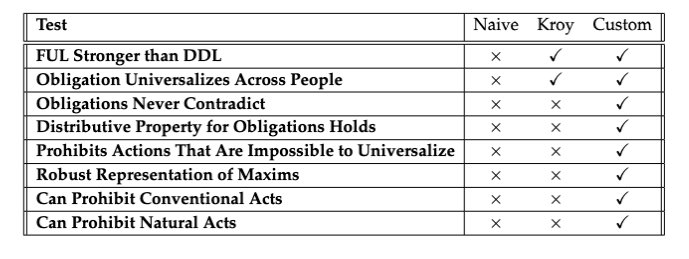
\includegraphics[scale=0.4]{goalstable.png}
\caption{Table indicating which goals are met by the naive formalization, Kroy's formalization, and 
the custom formalization respectively.} \label{fig:goalstable}
\end{figure}
%
\isadelimdocument
%
\endisadelimdocument
%
\isatagdocument
%
\isamarkupsubsubsection{Goals From Prior Attempts \label{sec:priorgoals}%
}
\isamarkuptrue%
%
\endisatagdocument
{\isafolddocument}%
%
\isadelimdocument
%
\endisadelimdocument
%
\begin{isamarkuptext}%
\textbf{FUL Stronger than DDL} One simple objective that the naive formalization failed to meet is the fact that the FUL should
not hold in the base logic (DDL). Recall that the naive formalization of the FUL\footnote{
This formalization reads $\vDash ((\neg (\square P \{A\})) \longrightarrow O \{\neg A\})$.} held in the 
base logic, so adding it as an axiom didn't make the logic any stronger. This is troubling 
because the base logic does not come equipped with the categorical imperative built-in. It 
defines basic properties of obligation, such as ought implies can, but contains no axioms that represent
the formula of universal law. Therefore, if a formalization of the FUL holds in the 
base logic, then it is too weak to actually represent the FUL. The naive interpretation holds in DDL but Kroy's formalization
does not. Because the naive interpretation is no stronger than DDL, it is acts a control group equivalent
to DDL itself.

\medskip 

\textbf{Obligation Universalizes Across People} Another property of the Formula of Universal Law that any implementation should satisfy is that obligation
generalizes across people. In other words, if a maxim is obligated for one person, it is obligated
for all other people because maxims are not person-specific. Velleman argues that, because 
reason is accessible to everyone identically, obligations apply to all people equually \cite[25]{velleman}. 
When Kant describes the categorical imperative as the objective principle of the will, he is referring 
to the fact that, as opposed to a subjective principle, the categorical imperative applies to all 
rational agents equally \cite[16]{groundwork}. At its core, the FUL best handles, ``the temptation 
to make oneself an exception: selfishness, meanness, advantagetaking, and disregard for the rights 
of others" \cite[30]{KorsgaardFUL}. Kroy latches onto this property and makes it the content of his
formalization, which essentially says that if an act is permissible for someone, it is permissible for 
everyone.\footnote{Formally, $P\{A(s)\} \longrightarrow \forall p. P\{A(p)\}$} While Kroy's interpretation 
clearly satisfies this property, the naive interpretation does not.

\medskip

\textbf{Contradictory Obligations} Another problem with prior formalizations was that they didn't
prohibit contradictory obligations, partially because DDL itself allows contradictory obligations. 
Kant subscribes to the general, popular view that morality is supposed to guide action, so ought implies 
can.\footnote{Kohl points out that this principle is referred to as 
Kant's dictum or Kant's law in the literature \cite[footnote 1]{kohl}.} Kohl reconstructs his argument for the principle as 
follows: if the will cannot comply with the moral law, then the moral law has no prescriptive authority 
for the will \cite[703-4]{kohl}. This defeats the purpose of Kant's theory—to develop an unconditional, categorical imperative 
for rational agents. Ought implies can requires that obligations never contradict, because an agent 
can't perform contradictory actions. Therefore, any ethical theory that respects ought implies can, 
and Kantian ethics in particular, must not result in conflicting obligations. 
Kant only briefly discusses contradictory obligations in \emph{Metaphysics of Morals}, where he argues that 
conflicting moral obligations are impossible under his theory \cite[V224]{metaphysicsintro}. Particularly, the categorical imperative generates 
``strict negative laws of omission," which cannot conflict by definition \cite[45]{timmerman}. \footnote{The 
kinds of obligations generated by the FUL are called ``perfect duties" which arise from ``contradictions 
in conception," or maxims that we cannot even concieve of universalizing. These duties are always negative 
and thus never conflict. Kant also presents ``imperfect duties," generated from ``contradictions in will,"
or maxims that we can concieve of universalizing but would never want to. These duties tend to be broader, 
such as ``improve oneself" or "help others," and are secondary to perfect duties. My project only analyzes 
perfect duties, as these are always stronger than imperfect duties.}. Both the naive formalization and 
Kroy's formalization allow contradictory obligations. 

During testing, I also realized that contradictory obligations are closely related to two other properties
that also fail in both of these systems. First is the idea that obligation implies permissibility, or 
that obligation is a stronger property than permissibility. If there are no contradictory obligations, 
then this property holds because actions are either permissible or prohibited and obligation contradicts
prohibition. Moreover, in a system with contradictory obligations, this property fails because there is some
A that is obligated but also prohibited and therefore not permisible. Indeed, formalizing this property below shows 
that this follows from the definition of implication in propositional logic.

\medskip%
\end{isamarkuptext}\isamarkuptrue%
\isacommand{lemma}\isamarkupfalse%
\ {\isachardoublequoteopen}{\isasymTurnstile}\ {\isacharparenleft}{\isacharparenleft}O\ {\isacharbraceleft}A{\isacharbraceright}\ \isactrlbold {\isasymand}\ O\ {\isacharbraceleft}\isactrlbold {\isasymnot}\ A{\isacharbraceright}{\isacharparenright}\ \isactrlbold {\isasymequiv}\ {\isacharparenleft}\isactrlbold {\isasymnot}\ {\isacharparenleft}O\ {\isacharbraceleft}A{\isacharbraceright}\ \isactrlbold {\isasymrightarrow}\ \isactrlbold {\isasymnot}\ O\ {\isacharbraceleft}\isactrlbold {\isasymnot}A{\isacharbraceright}{\isacharparenright}{\isacharparenright}{\isacharparenright}{\isachardoublequoteclose}\isanewline
%
\isadelimproof
\ \ %
\endisadelimproof
%
\isatagproof
\isacommand{by}\isamarkupfalse%
\ simp%
\endisatagproof
{\isafoldproof}%
%
\isadelimproof
%
\endisadelimproof
%
\begin{isamarkuptext}%
\textbf{Distributive Property} Another property related to contradictory obligations is the distributive property for the obligation
operator.\footnote{Formally, $O\{A\} \wedge O\{B\} \longleftrightarrow O\{A \wedge B\}$.} This is 
another property that we expect to hold. The rough English translation of  $O \{ A \wedge B \} $ is ``you are obligated to 
do both A and B". The rough English translation of $O\{A\} \wedge O\{B\}$ is ``you are obligated to do A 
and you are obligated to do B." We think those English sentences mean the same thing, so they should mean 
the same thing in logic as well. Moreover, if that (rather intuitive) property holds, then contradictory
obligations are impossible, as shown in the below proof.%
\end{isamarkuptext}\isamarkuptrue%
\isacommand{lemma}\isamarkupfalse%
\ distributive{\isacharunderscore}implies{\isacharunderscore}no{\isacharunderscore}contradictions{\isacharcolon}\ \isanewline
\ \ \isakeyword{assumes}\ {\isachardoublequoteopen}{\isasymforall}A\ B{\isachardot}\ {\isasymTurnstile}\ {\isacharparenleft}{\isacharparenleft}O\ {\isacharbraceleft}A{\isacharbraceright}\ \isactrlbold {\isasymand}\ O\ {\isacharbraceleft}B{\isacharbraceright}{\isacharparenright}\ \isactrlbold {\isasymequiv}\ O\ {\isacharbraceleft}A\ \isactrlbold {\isasymand}\ B{\isacharbraceright}{\isacharparenright}{\isachardoublequoteclose}\isanewline
\ \ \isakeyword{shows}\ {\isachardoublequoteopen}{\isasymforall}A{\isachardot}\ {\isasymTurnstile}{\isacharparenleft}\ \isactrlbold {\isasymnot}{\isacharparenleft}O\ {\isacharbraceleft}A{\isacharbraceright}\ \isactrlbold {\isasymand}\ O\ {\isacharbraceleft}\isactrlbold {\isasymnot}\ A{\isacharbraceright}{\isacharparenright}{\isacharparenright}\ {\isachardoublequoteclose}\isanewline
%
\isadelimproof
\ \ %
\endisadelimproof
%
\isatagproof
\isacommand{using}\isamarkupfalse%
\ O{\isacharunderscore}diamond\ assms\ \isacommand{by}\isamarkupfalse%
\ blast%
\endisatagproof
{\isafoldproof}%
%
\isadelimproof
%
\endisadelimproof
%
\begin{isamarkuptext}%
Thus, while testing contradictory obligations, I also test the distributive property for the 
obligation operator. Again, this property fails in the naive formalization and for Kroy's formalization.


\medskip 

\textbf{Un-universalizable Actions} This goal is inspired by a test performed for Kroy's formalization. Under 
a naive reading of the Formula of Universal Law, it prohibits lying because, in a world 
where everyone simultaneously lies, lying is impossible. In other words, not everyone can simultaneously
lie because the institution of lying and believing would break down. More precisely, the FUL should 
show that actions that cannot possibly be universalized are prohibited, because those acts cannot be willed in 
a world where they are universalized. This property fails to hold in both the naive formalization 
and Kroy's formalization and is a goal for my custom formalization.%
\end{isamarkuptext}\isamarkuptrue%
%
\isadelimdocument
%
\endisadelimdocument
%
\isatagdocument
%
\isamarkupsubsubsection{Goals From Philosophical Literature \label{sec:litgoals}%
}
\isamarkuptrue%
%
\endisatagdocument
{\isafolddocument}%
%
\isadelimdocument
%
\endisadelimdocument
%
\begin{isamarkuptext}%
The goals above come from moral intuition, properties of Kantian ethics, and logical requirements. 
In order to stay faithful to centuries of philosophical debate about the meaning of the Formula of 
Universl Law, I also present some goals inpsired by this literature.

\textbf{Maxims} Kant does not evaluate the correctness of acts, but rather of maxims. Therefore, any 
faithful formalization of the categorical imperative must evaluate maxims, not acts. This requires 
representing a maxim and making it the input to the obligation operator, which neither of the prior attempts do.

\medskip%
\end{isamarkuptext}\isamarkuptrue%
%
\begin{isamarkuptext}%
\textbf{Conventional Acts}
Kantians debate over the most philosophically sound interpretation of the Formula of Universal Law.
One litmus test that Korsgaard introduces makes a distinction between conventional and natural acts \citep{KorsgaardFUL}. 
A conventional act is one like promising, which relies on the convention of promising, in which we all
implicitly understand a promise as a commitment. Conventional acts are generally easier to show the 
wrongness of because there are worlds in which these acts are impossible; namely, worlds in which the 
convention does not exist. For example, the common argument against falsely promising is that if 
everyone were to falsely promise, the convention of promising would fall apart because people wouldn't believe
each other anymore, so falsely promising is prohibited. Despite the relative ease of this property,
it fails in both the naive and Kroy's interpretations, demonstrating the weakness of these 
formalizations. This property will hold for my custom formalization.

\medskip 

\textbf{Natural Acts}
The more difficult kind of act to show the wrongness of is a natural act, like murder or violence. 
These acts can never be logically impossible; even if everyone murders or acts violently, murder and 
violence will still be possible. This property of natural acts makes it difficult for interpretations of
the FUL to show the wrongness of violence. Both the naive and Kroy's interpretations fail to show
the wrongness of natural acts (in fact, they fail to show the weaker wrongness of conventional acts). 
This property will hold for the custom formalization. I will show the wrongness of both natural and 
conventional acts by formalizing Korsgaard's practical contradiction interpretation of the FUL, which 
is widely accepted as the canonical interpretation of the FUL \citep{KorsgaardFUL}. I will explain this 
decision in greater detail in the next chapter, where I present my custom formalization.%
\end{isamarkuptext}\isamarkuptrue%
%
\isadelimtheory
%
\endisadelimtheory
%
\isatagtheory
%
\endisatagtheory
{\isafoldtheory}%
%
\isadelimtheory
%
\endisadelimtheory
%
\end{isabellebody}%
\endinput
%:%file=~/Desktop/cs91r/paper/paper33.thy%:%
%:%24=6%:%
%:%36=8%:%
%:%37=9%:%
%:%38=10%:%
%:%39=11%:%
%:%40=12%:%
%:%41=13%:%
%:%42=14%:%
%:%43=15%:%
%:%44=16%:%
%:%45=17%:%
%:%46=18%:%
%:%47=19%:%
%:%50=22%:%
%:%51=23%:%
%:%52=24%:%
%:%53=25%:%
%:%54=26%:%
%:%55=27%:%
%:%63=29%:%
%:%75=31%:%
%:%76=32%:%
%:%77=33%:%
%:%78=34%:%
%:%79=35%:%
%:%80=36%:%
%:%81=37%:%
%:%82=38%:%
%:%83=39%:%
%:%84=40%:%
%:%85=41%:%
%:%86=42%:%
%:%87=43%:%
%:%88=44%:%
%:%89=45%:%
%:%90=46%:%
%:%91=47%:%
%:%92=48%:%
%:%93=49%:%
%:%94=50%:%
%:%95=51%:%
%:%96=52%:%
%:%97=53%:%
%:%98=54%:%
%:%99=55%:%
%:%100=56%:%
%:%101=57%:%
%:%102=58%:%
%:%103=59%:%
%:%104=60%:%
%:%105=61%:%
%:%106=62%:%
%:%107=63%:%
%:%108=64%:%
%:%109=65%:%
%:%110=66%:%
%:%111=67%:%
%:%112=68%:%
%:%113=69%:%
%:%114=70%:%
%:%115=71%:%
%:%116=72%:%
%:%117=73%:%
%:%118=74%:%
%:%119=75%:%
%:%120=76%:%
%:%121=77%:%
%:%122=78%:%
%:%123=79%:%
%:%124=80%:%
%:%125=81%:%
%:%126=82%:%
%:%127=83%:%
%:%128=84%:%
%:%129=85%:%
%:%130=86%:%
%:%131=87%:%
%:%132=88%:%
%:%134=92%:%
%:%135=92%:%
%:%138=93%:%
%:%142=93%:%
%:%143=93%:%
%:%152=95%:%
%:%153=96%:%
%:%154=97%:%
%:%155=98%:%
%:%156=99%:%
%:%157=100%:%
%:%158=101%:%
%:%160=103%:%
%:%161=103%:%
%:%162=104%:%
%:%163=105%:%
%:%166=106%:%
%:%170=106%:%
%:%171=106%:%
%:%172=106%:%
%:%181=108%:%
%:%182=109%:%
%:%183=110%:%
%:%184=111%:%
%:%185=112%:%
%:%186=113%:%
%:%187=114%:%
%:%188=115%:%
%:%189=116%:%
%:%190=117%:%
%:%191=118%:%
%:%192=119%:%
%:%193=120%:%
%:%202=122%:%
%:%214=124%:%
%:%215=125%:%
%:%216=126%:%
%:%217=127%:%
%:%218=128%:%
%:%219=129%:%
%:%220=130%:%
%:%221=131%:%
%:%222=132%:%
%:%226=136%:%
%:%227=137%:%
%:%228=138%:%
%:%229=139%:%
%:%230=140%:%
%:%231=141%:%
%:%232=142%:%
%:%233=143%:%
%:%234=144%:%
%:%235=145%:%
%:%236=146%:%
%:%237=147%:%
%:%238=148%:%
%:%239=149%:%
%:%240=150%:%
%:%241=151%:%
%:%242=152%:%
%:%243=153%:%
%:%244=154%:%
%:%245=155%:%
%:%246=156%:%
%:%247=157%:%
%:%248=158%:%
%:%249=159%:%
%
\begin{isabellebody}%
\setisabellecontext{paper{\isadigit{4}}{\isadigit{1}}}%
%
\isadelimtheory
%
\endisadelimtheory
%
\isatagtheory
%
\endisatagtheory
{\isafoldtheory}%
%
\isadelimtheory
%
\endisadelimtheory
%
\isadelimdocument
%
\endisadelimdocument
%
\isatagdocument
%
\isamarkupsection{Novel Formalization of the Categorical Imperative%
}
\isamarkuptrue%
%
\endisatagdocument
{\isafolddocument}%
%
\isadelimdocument
%
\endisadelimdocument
%
\begin{isamarkuptext}%
In this section, I present a custom formalization of the categorical imperative, as inspired by 
the goals from the previous chapter.%
\end{isamarkuptext}\isamarkuptrue%
%
\isadelimdocument
%
\endisadelimdocument
%
\isatagdocument
%
\isamarkupsubsection{Logical Background%
}
\isamarkuptrue%
%
\endisatagdocument
{\isafolddocument}%
%
\isadelimdocument
%
\endisadelimdocument
%
\begin{isamarkuptext}%
The previous attempts to model the categorical imperative in Chapter 2 partially failed due to 
an inability to fully represent the complexity of a maxim. Specifically, they treated actions as a single, 
monolithic unit of evaluation, whereas most Kantians consider the unit of evaluation for the FUL to the more
complex notion of a maxim. In this section, I will present some logical background necessarily to fully 
capture the spirit of a maxim. I will begin by borrowing some machinery to handle ``subjects" who perform 
actions from Chapter 2.%
\end{isamarkuptext}\isamarkuptrue%
\isacommand{typedecl}\isamarkupfalse%
\ s\ %
\isamarkupcmt{s is the type for a ``subject," i.e. the subject of a sentence. In this interpretation, 
a subject is merely defined as ``that which can act." It does not include any other properties, such as 
rationality or dignity. As I will show, for the purposes of defining the universalizability test, this 
``thin" representation of a subject suffices.%
}\isanewline
\isanewline
\isacommand{type{\isacharunderscore}synonym}\isamarkupfalse%
\ os\ {\isacharequal}\ {\isachardoublequoteopen}{\isacharparenleft}s\ {\isasymRightarrow}\ t{\isacharparenright}{\isachardoublequoteclose}\ %
\isamarkupcmt{Recall that an open sentence maps a subject to a term to model the 
substitution operator.%
}\isanewline
\isanewline
\isacommand{type{\isacharunderscore}synonym}\isamarkupfalse%
\ maxim\ {\isacharequal}\ {\isachardoublequoteopen}{\isacharparenleft}t\ {\isacharasterisk}\ os\ {\isacharasterisk}\ t{\isacharparenright}{\isachardoublequoteclose}%
\begin{isamarkuptext}%
The central unit of evaluation for the universalizability test is a ``maxim," which Kant defines 
in a footnote in \emph{Groundwork} as ``the subjective principle of willing," or the principle that 
the agent acts on $\cite[16]{groundwork}$. Modern Kantians differ in their interpretations of this definition. The naive view 
is that a maxim is an act, but Korsgaard adopts the more sophisticated view that a maxim is composed
of an act and the agent's purpose for acting \cite{actingforareason}. She also compares a maxim 
to Aristotle's logos, which includes these components and information about the circumstances and methods 
of the act. O'Neill concludes that Kant's examples imply that a maxim must also include circumstances \cite{actingonprinciple}, and 
Kitcher \cite{whatisamaxim} uses textual evidence from the Groundwork to argue for the inclusion of a maxim's purpose 
or motivation. In order to formalize the notion of a maxim, I must adopt a specific definition and 
defend my choice.

I define a maxim as a circumstance, act, goal tuple (C, A, G), read 
as ``In circumstances C, act A for goal G." Isabelle's strict typing rules mean that the choice of the 
type of each member of this tuple is significant. A circumstance is represented as a set of worlds 
$t$ where that circumstance holds. A goal is also a term because it can be true or false at a world if it 
is realized or not. An act is an open sentence because an act itself is not the kind of thing that can 
be true or false (as in, an act is not truth-apt), but the combination of a subject performing an act 
can be true or false at a world depending on whether or not the act is indeed performed by that subject. 
For example, ``running" is not truth-apt, but ``Sara runs" is truth-apt.

My definition of a maxim is inspired by O'Neill's work on maxims. I will defend my representation
below and consider an additional component that Kitcher argues for.

$\emph{O'Niell's Original Schematic and The Role of Practical Judgement}$

O'Neill $\cite[37]{actingonprinciple}$ presents what Kitcher \cite{whatisamaxim}  calls the widely accepted 
view that a maxim is a circumstance, act, goal tuple. A maxim 
is an action-guiding rule and thus naturally includes an act and the circumstances under which 
it should be performed, which are often referred to as ``morally relevant circumstances." 

She also includes a purpose, end, or goal in the maxim because Kant includes this in many of his 
example maxims and because Kant argues that human activity, because it is guided by a rational will, 
is inherently purposive $\cite[4:428]{groundwork}$. A rational will does not act randomly (else it would not be rational), 
but instead in the pursuit of ends which it deems valuable. This inclusion is also essential for the version of the universalizability test 
that I will implement, explained in Section ??.

O'Neill's inclusion of circumstances is potentially controversial because it leaves open the question of what qualifies as a 
relevant circumstance for a particular maxim. This is gives rise to ``the tailoring objection" $\cite[217]{whatisamaxim} \footnote{Kitcher
cites \cite{kantsethicalthought}  as offering an example of a false positive due to this objection.}$, 
under which maxims are arbitrarily specified to pass the FUL. For example, the maxim ``When my name is Lavanya Singh,
I will lie to get some easy money," is universalizable, but is clearly a false positive. One solution to 
this problem is to argue that the circumstance ``When my name is Lavanya Singh" is not morally relevant 
to the act and goal. This solution requires some discussion of what qualifies as a relevant circumstance.

O'Neill seems to acknowledge the difficulty of determining relevant circumstances when she concedes that a maxim cannot include all 
of the infinitely many circumstances in which the agent may perform the action$\cite[4:428]{actingonprinciple}$. She argues that this is 
an artifact of the fact that maxims are rules of practical reason, the kind of reason that helps us decide what to do 
and how to do it \cite{bok}. Like any practical rule, 
maxims require the exercise of practical judgement to determine in which circumstances they should be applied. 
This judgement, applied in both choosing when to exercise the maxim and in the formulation of the maxim 
itself, is what determines the ``morally relevant circumstances."

The upshot for computational ethics is that the computer cannot perform all ethical activity alone. 
Human judgement and the exercise of practical reason are essential to both formulate maxims and 
determine when the actual conditions of life coincide with the circumstances in which the maxim is relevant. 
Choosing when to exercise a maxim is less relevant to my project because analyzing a formal representation of the FUL requires 
making the circumstances in a given scenario precise, but will be important for applications of 
computational ethics to guiding AI agents. The difficulty in formulating a maxim, on the other hand, demonstrates 
the important fact that ethics, as presented here, is not a solely computational activity. A
human being must create a representation for the dilemma they wish to test, effectively translating 
a complex, real situation into a flat logical structure. This parallels the challenge that programmers 
face when translating the complexity of reality to a programming langauge or computational representation. Not only will some of the situation's complexity
inevitably be lost, the outcome of the universalizability test will depend on how the human formulates the maxim
and whether or not this formulation does indeed include morally relevant circumstances. If the human puts 
garbage into the test, the test will return garbage out.

While this may appear to be a weakness of my system, I believe that it actually
allows my system to retain some of the human complexity that many philosophers agree cannot be automated away.\footnote{Powers presents 
the determination of morally relevant circumstances as an obstacle to the automation of Kantian ethics \cite{powers}.}
Ethics is a fundamentally human activity. Kant argues that the categorical imperative is a statement 
about the properties of rational wills. In fact, Korsgaard argues that morality derives its authority over us, 
or normativity, only because is it a property of a rational will, and we, as human beings, are rational wills.
If ethics is meant to guide human behavior, the role of the computer becomes clear as not a replacement for our will,
but instead as a tool to help guide our wills and reason more efficiently 
and more effectively. Just as calculators don't render mathematicians obsolete, computational ethics
does not render human judgement or philosophy obsolete. Chapter 4 Section ?? will be devoted to a more complete discussion 
of this issue.

$\emph{Exclusion of Motive}$

Kitcher begins with O'Niell's circumstance, act, goal view and expands it to include the motive 
behind performing the maxim \cite{whatisamaxim}. This additional component is read 
as ``In circumstance C, I will do A in order to G because of M," where M may be ``duty" or ``self-love."
Kitcher argues that the inclusion of motive is necessary for the fullest, most general form of a maxim
in order to capture Kant's idea that an action derives its moral worth from being done for the sake of duty itself.
Under this view, the FUL would obligate maxims of the form 
``In circumstance C, I will do A in order to G because I can will that I and everyone else simultaneously
will do A in order to G in circumstance C." In other words, if Kant is correct in arguing that moral 
actions must be done from the motive of duty, the affirmative result of the FUL becomes 
the motive for a moral action.

While Kitcher's conception of a maxim captures Kant's idea of acting for duty's own sake, I will not implement it 
because it is not necessary for putting maxims through the FUL. Indeed, Kitcher acknowledges that 
O'Neill's formulation suffices for the universalizability test, but is not the general notion of a maxim.
In order to pass the maxim through the FUL, it suffices to know the circumstance, act, and goal. The FUL
derives the motive that Kitcher bundles into the maxim, so automating the FUL does not require 
including a motive. The ``input" to the FUL is the circumstance, act, goal tuple. My project takes 
this input and returns the motivation that the dutiful, moral agent would adopt. Additionally, doing
justice to the rich notion of motive requires modelling the operation of practical reason itself, 
which is outside the scope of this project. My work focuses on the universalizability test, but future work that 
models the process of practical reason may use my implementation of the FUL as a ``library." Combined 
with a logic of practical reason, an implementation of the FUL can move from evaluating a maxim to 
evaluating an agent's behavior, since that's when ``acting from duty" starts to matter.%
\end{isamarkuptext}\isamarkuptrue%
\isacommand{abbreviation}\isamarkupfalse%
\ will\ {\isacharcolon}{\isacharcolon}\ {\isachardoublequoteopen}maxim\ {\isasymRightarrow}\ s{\isasymRightarrow}\ \ t{\isachardoublequoteclose}\ {\isacharparenleft}{\isachardoublequoteopen}W\ {\isacharunderscore}\ {\isacharunderscore}{\isachardoublequoteclose}{\isacharparenright}\isanewline
\ \ \isakeyword{where}\ {\isachardoublequoteopen}will\ {\isasymequiv}\ {\isasymlambda}{\isacharparenleft}c{\isacharcomma}\ a{\isacharcomma}\ g{\isacharparenright}\ s{\isachardot}\ {\isacharparenleft}c\ \isactrlbold {\isasymrightarrow}\ {\isacharparenleft}a\ s{\isacharparenright}{\isacharparenright}{\isachardoublequoteclose}\isanewline
\isacommand{print{\isacharunderscore}theorems}\isamarkupfalse%
%
\begin{isamarkuptext}%
Korsgaard claims that ``to will an end, rather than just
wishing for it or wanting it, is to set yourself to be its cause" \cite[38]{sources}. To will a maxim
is to set yourself to be the cause of its goal by taking the means 
specified in the maxim in the relevant circumstances. This coheres with 
Kitcher's and Korsgaard's understanding of a maxim as a principle or rule to live by. 

At worlds
where the circumstances do not hold, a maxim is vacuously willed. If you decide to act on the rule ``I will 
do X in these cirumstances", then you are vacuously obeying it when the circumstances don't hold.  

The above discussion implies that willing a maxim is particular to the agent, justifying my choice to 
require that a particular subject will a maxim. O'Neill argues for this interpretation when she distinguishes 
between the evaluation of a principle, which is generic, and a maxim, which she views as ``individuated only 
by referring to a person"$\cite[13]{actingonprinciple}$. I adopt the spirit of this interpretation but modify it slightly 
by representing the general maxim as a principle that anyone could adopt, and the act of willing the maxim 
as a person-particular instantiation of the maxim.

I additionally represent a subject as willing a maxim because I use the word `will' as a verb, to mean committing oneself to living by
the principle of a maxim. This coheres with the FUL, which tests the act willing 
of a maxim by determining if the maxim could be a universal law that everyone committed to. Formalizing this idea,
the type of a willed maxim is a term, allowing me
to use DDL's obligation operator on the notion of willing a maxim. Concretely, my system will prove 
or disprove statements of the form ``Lavanya is obligated to will the maxim M." 

Worlds where the circumstances do not hold are not relevant for determining obligation. Recall that in 
Benzmueller et. al's definition of the obligation operator,  $O \{B|A\}$ is true at all worlds iff ob(B)(A), or 
if the obligation function maps A to obligatory in context B (where the context is a set of worlds) \cite{BFP}. This 
definition implies that worlds outside of B have no bearing on the moral status of A in context B, which 
coheres with intuitions about contextual obligation. Thus, the dyadic obligation operator 
disqualifies worlds where the context does not hold, so the vacuous truth of the will statement in 
these worlds does not matter. 

Given that the will abbreviation already excludes worlds where the circumstances fail (by rendering 
the statement vacuously true at them), one may conclude that the dyadic obligation operator is now useless. 
Using the dyadic obligation operator allows me to take advantage of the power of DDL to represent the bearing 
that circumstances have on obligation. DDL has powerful axioms expressing the relationship between circumstances 
and obligation, such as the fact that obligations are monotonically increasing with respect to broader 
circumstances. Using the monadic obligation operator would require me to either operate with an empty 
notion of context or to redefine these axioms. The dyadic obligation operator lets me take advantage of the full 
power of DDL in expressing contrary-to-duty obligations. This is particularly important for Kantian ethics 
and the FUL specifically because many critiques of the FUL rely on attention to circumstances (tailoring 
objection) or lack thereof (ideal theory). This is also an innovation that my custom formalization presents 
over the prior work. By formally including the notion of a circumstance or context, I am able to represent 
these objections that Kantian scholars study. Formalizing Kantian ethics in a dyadic deontic logic 
instead of a monadic deontic logic is a key contribution of this thesis.%
\end{isamarkuptext}\isamarkuptrue%
\isacommand{abbreviation}\isamarkupfalse%
\ effective\ {\isacharcolon}{\isacharcolon}\ {\isachardoublequoteopen}maxim{\isasymRightarrow}s{\isasymRightarrow}\ t{\isachardoublequoteclose}\ {\isacharparenleft}{\isachardoublequoteopen}E\ {\isacharunderscore}\ {\isacharunderscore}{\isachardoublequoteclose}{\isacharparenright}\isanewline
\ \ \isakeyword{where}\ {\isachardoublequoteopen}effective\ \ {\isasymequiv}\ {\isasymlambda}{\isacharparenleft}c{\isacharcomma}\ a{\isacharcomma}\ g{\isacharparenright}\ s{\isachardot}\ {\isacharparenleft}{\isacharparenleft}will\ {\isacharparenleft}c{\isacharcomma}\ a{\isacharcomma}\ g{\isacharparenright}\ s{\isacharparenright}\ \isactrlbold {\isasymequiv}\ g{\isacharparenright}{\isachardoublequoteclose}\isanewline
\isacommand{print{\isacharunderscore}theorems}\isamarkupfalse%
%
\begin{isamarkuptext}%
A maxim is effective for a subject when, if the subject wills it then the goal is achieved, and
when the subject does not act on it, the goal is not achieved$\footnote{Thank you to Jeremy D. Zucker for helping me think through this.}$ \cite{sepcausation}. 
The former direction of the implication 
is intuitive: if the act results in the goal, it was effective in causing the goal. This represents `necessary'
causality. 

The latter direction represents `sufficient' causality, or the idea that, counterfactually,
if the maxim were not willed, then the goal is not achieved \cite{lewiscausality}. Note that nothing else changes about this
counterfactual world—the circumstances are identical and we neither added additional theorems nor 
specified the model any further. This represents Lewis's idea of "comparative similarity,"  where 
a counterfactual is true if it holds at the most similar world \cite{lewiscounterfactuals}. In our case, this is just the world 
where everything is the same except the maxim is not acted on.

Combining these ideas, this definition of effective states that a maxim is effective if the 
maxim being acted on by a subject is the necessary and sufficient cause of the goal.\footnote{Should I wave a hand at critiques of counterfactual causality?}

If the circumstances do not hold and the goal is achieved, then the maxim is vacuously effective, since 
it is vacuously willed (as described above). While this scenario is counterintuitive, it is not very 
interesting for my purposes because, when the circumstances do not hold, a maxim is not applicable. It 
doesn't really make sense to evaluate a maxim when it's not supposed to be applied. The maxim ``When on Jupiter,
read a book to one-up your nemesis" is vacuously effective because it can never be disproven.%
\end{isamarkuptext}\isamarkuptrue%
\isacommand{abbreviation}\isamarkupfalse%
\ universalized{\isacharcolon}{\isacharcolon}{\isachardoublequoteopen}maxim{\isasymRightarrow}s{\isasymRightarrow}t{\isachardoublequoteclose}\ \isakeyword{where}\ \isanewline
{\isachardoublequoteopen}universalized\ {\isasymequiv}\ {\isasymlambda}M\ s{\isachardot}\ {\isacharparenleft}{\isasymlambda}w{\isachardot}\ {\isacharparenleft}{\isasymforall}p{\isachardot}\ W\ M\ p\ w{\isacharparenright}{\isacharparenright}{\isachardoublequoteclose}\isanewline
\isanewline
\isacommand{abbreviation}\isamarkupfalse%
\ not{\isacharunderscore}universalizable\ {\isacharcolon}{\isacharcolon}\ {\isachardoublequoteopen}maxim{\isasymRightarrow}s{\isasymRightarrow}bool{\isachardoublequoteclose}\ \isakeyword{where}\ \isanewline
{\isachardoublequoteopen}not{\isacharunderscore}universalizable\ {\isasymequiv}\ {\isasymlambda}M\ s{\isachardot}\ {\isacharparenleft}{\isasymTurnstile}\ {\isacharparenleft}universalized\ M\ s\ \isactrlbold {\isasymrightarrow}\ {\isacharparenleft}\isactrlbold {\isasymnot}\ {\isacharparenleft}E\ M\ s{\isacharparenright}{\isacharparenright}{\isacharparenright}{\isacharparenright}{\isachardoublequoteclose}\isanewline
%
\isamarkupcmt{The maxim willed by subject $s$ is not universalizable if, for all people $p$, if $p$ wills M, then 
$M$ is no longer effective for $s$.%
}%
\begin{isamarkuptext}%
As before, the concepts of prohibition and permissibility will be helpful here. The unit of 
evaluation for my formalization of the FUL is the act of willing a maxim, which entails performing 
the maxim's act in the relevant circumstances. Therefore, I will say that, just as the act of willing a
 maxim can be obligatory for a subject, it can be prohibited or permissible for a subject.\footnote{In 
the rest of this section, for convenience, I will use the phrase ``subject s willing maxim M is obligatory" 
interchangeably with ``maxim M is obligatory for subject s." I will use ``maxim M is obligatory" to 
refer to M being obligatory for any arbitrary subject, which I will show to be equivalent to M being 
obligatory for a specific subject.}%
\end{isamarkuptext}\isamarkuptrue%
\isacommand{abbreviation}\isamarkupfalse%
\ prohibited{\isacharcolon}{\isacharcolon}{\isachardoublequoteopen}maxim{\isasymRightarrow}s{\isasymRightarrow}t{\isachardoublequoteclose}\ \isakeyword{where}\ \isanewline
{\isachardoublequoteopen}prohibited\ {\isasymequiv}\ {\isasymlambda}{\isacharparenleft}c{\isacharcomma}\ a{\isacharcomma}\ g{\isacharparenright}\ s{\isachardot}\ O{\isacharbraceleft}\isactrlbold {\isasymnot}\ {\isacharparenleft}will\ {\isacharparenleft}c{\isacharcomma}a{\isacharcomma}\ g{\isacharparenright}\ s{\isacharparenright}\ {\isacharbar}\ c{\isacharbraceright}{\isachardoublequoteclose}\isanewline
\isanewline
\isacommand{abbreviation}\isamarkupfalse%
\ permissible{\isacharcolon}{\isacharcolon}{\isachardoublequoteopen}maxim{\isasymRightarrow}s{\isasymRightarrow}t{\isachardoublequoteclose}\isanewline
\ \ \isakeyword{where}\ {\isachardoublequoteopen}permissible\ {\isasymequiv}\ {\isasymlambda}M\ s{\isachardot}\ \isactrlbold {\isasymnot}\ {\isacharparenleft}prohibited\ M\ s{\isacharparenright}{\isachardoublequoteclose}\isanewline
%
\isamarkupcmt{I will say that a maxim is permissible for a subject if it is not prohibited for that subject to 
will that maxim.%
}%
\begin{isamarkuptext}%
One problem with prior formalization of the categorical imperative was that they didn't
prohibit contradictory obligations, partially because DDL itself allows contradictory obligations. 
Kant subscribes to the general, popular view that morality is supposed to guide action, so ought implies 
can\footnote{Kohl points out that this principle is referred to as 
Kant's dictum or Kant's law in the literature. \cite[footnote 1]{kohl}}. Kohl reconstructs his argument for the principle as 
follows: if the will cannot comply with the moral law, then the moral law has no prescriptive authority 
for the will \cite[703-4]{kohl}. This defeats the purpose of Kant's theory—to develop an unconditional, categorical imperative 
for rational agents. Ought implies can requires that obligations never contradict, because an agent 
can't perform contradictory actions. Therefore, any ethical theory that respects ought implies can, 
and Kantian ethics in particular, must not result in conflicting obligations.

Kant only briefly discusses contradictory obligations in \emph{Metaphysics of Morals}, where he argues that 
conflicting moral obligations are impossible under his theory \cite[V224]{metaphysicsintro}. Particularly, the categorical imperative generates 
``strict negative laws of omission", which cannot conflict by definition \cite[45]{timmerman}.\footnote{The 
kinds of obligations generated by the FUL are called ``perfect duties" which arise from ``contradictions 
in conception," or maxims that we cannot even concieve of universalizing. These duties are always negative 
and thus never conflict. Kant also presents ``imperfect duties," generated from ``contradictions in will,"
or maxims that we can concieve of universalizing but would never want to. These duties tend to be broader, 
such as ``improve oneself" or "help others," and are secondary to perfect duties. My project only analyzes 
perfect duties, as these are stronger than imperfect duties.} 

When analyzing the naive formalization and Kroy's formalization, I learned that DDL and the prior 
formalizations allow contradictory obligations. This is a major weakness of these systems, and my 
formalization should fix this. To do so, I will add as an axiom the idea that obligations cannot 
contradict each other or their internal circumstances. Formally, conflicting obligations are defined below.%
\end{isamarkuptext}\isamarkuptrue%
\isacommand{abbreviation}\isamarkupfalse%
\ non{\isacharunderscore}contradictory\ \isakeyword{where}\ \isanewline
{\isachardoublequoteopen}non{\isacharunderscore}contradictory\ A\ B\ c\ w\ {\isasymequiv}\ {\isacharparenleft}{\isacharparenleft}O{\isacharbraceleft}A{\isacharbar}c{\isacharbraceright}\ \isactrlbold {\isasymand}\ O{\isacharbraceleft}B{\isacharbar}c{\isacharbraceright}{\isacharparenright}\ w{\isacharparenright}\ {\isasymlongrightarrow}\ {\isasymnot}{\isacharparenleft}{\isacharparenleft}A\ \isactrlbold {\isasymand}\ {\isacharparenleft}B\ \isactrlbold {\isasymand}\ c{\isacharparenright}{\isacharparenright}\ w\ {\isasymlongrightarrow}\ False{\isacharparenright}{\isachardoublequoteclose}\isanewline
%
\isamarkupcmt{Terms A and B are non contradictory in circumstances c if, when A and B are obligated in circumstances 
c, the conjunction of A, B, and c, does not imply False.%
}\isanewline
\isanewline
\isacommand{axiomatization}\isamarkupfalse%
\ \isakeyword{where}\ no{\isacharunderscore}contradictions{\isacharcolon}{\isachardoublequoteopen}{\isasymforall}A{\isacharcolon}{\isacharcolon}t{\isachardot}\ {\isasymforall}B{\isacharcolon}{\isacharcolon}t{\isachardot}\ {\isasymforall}c{\isacharcolon}{\isacharcolon}t{\isachardot}\ {\isasymforall}w{\isacharcolon}{\isacharcolon}i{\isachardot}\ non{\isacharunderscore}contradictory\ A\ B\ c\ w{\isachardoublequoteclose}\isanewline
%
\isamarkupcmt{This axiom formalizes the idea that, for any terms A, B, and circumstances c, A and B must be 
non-contradictory in circumstances c at all worlds. Intuitively, this axiom requires that obligations 
do not conflict.%
}%
\isadelimdocument
%
\endisadelimdocument
%
\isatagdocument
%
\isamarkupsubsection{Formalizing the FUL%
}
\isamarkuptrue%
%
\endisatagdocument
{\isafolddocument}%
%
\isadelimdocument
%
\endisadelimdocument
%
\begin{isamarkuptext}%
Below is my first attempt at formalizing Korgsaard's definition of the practical contradiction
interpretation:  a maxim is not universalizable 
if, in the world where the maxim becomes the standard practice (i.e. everyone acts on the maxim), the
agent's attempt to use the maxim's act to achieve the maxim's goal is frustrated. In other words, if 
the maxim is universally willed (captured by applying a universal qunatifier and the will function 
to the maxim on the LHS), then it is no longer effective for the subject $s$ (RHS above).%
\end{isamarkuptext}\isamarkuptrue%
\isacommand{abbreviation}\isamarkupfalse%
\ FUL{\isadigit{0}}{\isacharcolon}{\isacharcolon}bool\ \isakeyword{where}\ {\isachardoublequoteopen}FUL{\isadigit{0}}\ {\isasymequiv}\ {\isasymforall}\ c\ a\ g\ s{\isachardot}\ not{\isacharunderscore}universalizable\ {\isacharparenleft}c{\isacharcomma}\ a{\isacharcomma}\ g{\isacharparenright}\ s\ {\isasymlongrightarrow}\ {\isasymTurnstile}{\isacharparenleft}{\isacharparenleft}prohibited\ {\isacharparenleft}c{\isacharcomma}\ a{\isacharcomma}\ g{\isacharparenright}\ s{\isacharparenright}{\isacharparenright}{\isachardoublequoteclose}\isanewline
%
\isamarkupcmt{This representation of the Formula of Universal Law reads, ``For all circumstances, goals, acts, 
and subjects, if the maxim of the subject performing the act for the goal in the circumstances is not 
universalizable (as defined above), then, at all worlds, in those circumstances, the subject 
is prohibited (obligated not to) from willing the maxim.%
}\isanewline
\isanewline
\isacommand{lemma}\isamarkupfalse%
\ {\isachardoublequoteopen}FUL{\isadigit{0}}\ {\isasymlongrightarrow}\ False{\isachardoublequoteclose}%
\isadelimproof
\ %
\endisadelimproof
%
\isatagproof
\isacommand{using}\isamarkupfalse%
\ O{\isacharunderscore}diamond\ \isanewline
\ \ \isacommand{using}\isamarkupfalse%
\ prod{\isachardot}simps{\isacharparenleft}{\isadigit{2}}{\isacharparenright}\ split{\isacharunderscore}conv\ \isacommand{by}\isamarkupfalse%
\ fastforce%
\endisatagproof
{\isafoldproof}%
%
\isadelimproof
%
\endisadelimproof
%
\begin{isamarkuptext}%
FUL0 is not consistent, and sledgehammer is able to prove this by showing that it implies a contradiction 
usig axiom O\_diamond, which is \isa{{\isasymTurnstile}{\isasymlambda}w{\isachardot}\ ob\ {\isacharquery}B\ {\isacharquery}A\ {\isasymlongrightarrow}\ {\isasymnot}\ {\isasymTurnstile}\isactrlbold {\isasymnot}\ {\isacharquery}B\isactrlbold {\isasymand}{\isacharquery}A}. This axiom captures 
the idea that an obligation can't contradict its context. This is particularly problematic if the goal or 
action of a maxim are equivalent to its circumstances. In other words, if the maxim has already been 
acted on or the goal has already been achieved, then prohibiting it is impossible. 
In any model that has at least one term, it is possible to construct a maxim where the circumstances, goal, 
and act (once a subject acts on it) are all that same term, resulting in a contradiction. 

To get around this, I will exclude what I call ``badly formed maxims," which are those maxims such that the goal has already been 
achieved or the act has already been acted on. Under my formalization, such maxims are 
not well-formed. To understand why, I return to Korsgaard's and O'Neill's interpretations of a maxim as a practical
guide to action. A maxim is a practical principle that guides how we behave in everyday life. A 
principle of the form ``When you are eating breakfast, eat breakfast in order to eat breakfast," is not 
practically relevant. No agent would ever need to act on such a principle. It is not contradictory
or prohibited, but it is the wrong kind of question to be asking. It is not a 
well-formed maxim, so the categorical imperative does not apply to it. (more explanation in philosophical 
writing collection)%
\end{isamarkuptext}\isamarkuptrue%
\isacommand{abbreviation}\isamarkupfalse%
\ well{\isacharunderscore}formed{\isacharcolon}{\isacharcolon}{\isachardoublequoteopen}maxim{\isasymRightarrow}s{\isasymRightarrow}i{\isasymRightarrow}bool{\isachardoublequoteclose}\ \isakeyword{where}\ \isanewline
{\isachardoublequoteopen}well{\isacharunderscore}formed\ {\isasymequiv}\ {\isasymlambda}{\isacharparenleft}c{\isacharcomma}\ a{\isacharcomma}\ g{\isacharparenright}\ s\ w{\isachardot}\ {\isacharparenleft}{\isasymnot}\ {\isacharparenleft}\ {\isacharparenleft}c\ \isactrlbold {\isasymrightarrow}\ g{\isacharparenright}\ w{\isacharparenright}{\isacharparenright}\ {\isasymand}\ {\isacharparenleft}{\isasymnot}\ {\isacharparenleft}\ {\isacharparenleft}c\ \isactrlbold {\isasymrightarrow}\ a\ s{\isacharparenright}\ w{\isacharparenright}{\isacharparenright}{\isachardoublequoteclose}\isanewline
%
\isamarkupcmt{This abbreviation formalizes the well-formedness of a maxim for a subject. The goal cannot be 
already achieved in the circumstances and the subject cannot have already performed the act.%
}\isanewline
\isanewline
\isacommand{abbreviation}\isamarkupfalse%
\ FUL\ \isakeyword{where}\ {\isachardoublequoteopen}FUL\ {\isasymequiv}\ {\isasymforall}M{\isacharcolon}{\isacharcolon}maxim{\isachardot}\ {\isasymforall}s{\isacharcolon}{\isacharcolon}s{\isachardot}\ {\isacharparenleft}{\isasymforall}w{\isachardot}\ well{\isacharunderscore}formed\ M\ s\ w{\isacharparenright}\ {\isasymlongrightarrow}\ {\isacharparenleft}not{\isacharunderscore}universalizable\ M\ s\ {\isasymlongrightarrow}\ {\isasymTurnstile}\ prohibited\ M\ s\ {\isacharparenright}{\isachardoublequoteclose}\isanewline
%
\isamarkupcmt{Let's try the exact same formalization of the FUL as above, except that it only applies to 
maxims that are well-formed at every world.%
}\isanewline
\isanewline
\isacommand{lemma}\isamarkupfalse%
\ {\isachardoublequoteopen}FUL{\isachardoublequoteclose}\isanewline
\ \ \isacommand{nitpick}\isamarkupfalse%
{\isacharbrackleft}user{\isacharunderscore}axioms{\isacharcomma}\ falsify{\isacharequal}true{\isacharbrackright}%
\isadelimproof
\ %
\endisadelimproof
%
\isatagproof
\isacommand{oops}\isamarkupfalse%
\isanewline
%
\isamarkupcmt{The FUL does not hold in DDL, because nitpick is able to find a model for my system in which it is 
false. If the FUL were already a theorem of the system, adding it wouldn't make the system any more 
powerful, so this is the desired result.

$\color{blue}$ Nitpick found a counterexample for card s = 1 and card i = 1:

  Skolem constants:
    M = (($\lambda x. \_$)($i_1$ := True), ($\lambda x. \_$)($s_1$ := ($\lambda x. \_$)($i_1$ := False)), ($\lambda x. \_$)
         ($i_1$ := False))
    $\lambda$ w. p = ($\lambda x. \_$)($i_1$ := $s_1$)
    s = $s_1$ $\color{black}$%
}%
\endisatagproof
{\isafoldproof}%
%
\isadelimproof
%
\endisadelimproof
\isanewline
\isanewline
\isacommand{axiomatization}\isamarkupfalse%
\ \isakeyword{where}\ FUL{\isacharcolon}FUL\isanewline
\isanewline
\isacommand{lemma}\isamarkupfalse%
\ True\isanewline
\ \ \isacommand{nitpick}\isamarkupfalse%
{\isacharbrackleft}user{\isacharunderscore}axioms{\isacharcomma}\ falsify{\isacharequal}false{\isacharbrackright}%
\isadelimproof
\ %
\endisadelimproof
%
\isatagproof
\isacommand{by}\isamarkupfalse%
\ simp\isanewline
%
\isamarkupcmt{Nitpick is able to find a model in which all axioms are satisfied, 
so this version of the FUL is consistent.

$\color{blue}$ Nitpick found a model for card i = 1 and card s = 1:

  Empty assignment $\color{black}$%
}%
\endisatagproof
{\isafoldproof}%
%
\isadelimproof
%
\endisadelimproof
%
\begin{isamarkuptext}%
During the process of making FUL0 consistent, I used Isabelle to gain philosophical insights 
about vacuous maxims. This process is an example of the power of computational tools to aid
philosophical progress. I used Nitpick and Sledgehammer to quickly test if a small tweak 
to FUL0 fixed the inconsistency or if I was still able to derive a contradiction.  I then realized that if 
I defined the circumstances, act, and goal as constants, then FUL0 was indeed consistent. After some 
experimentation, Prof. Amin correctly pointed out that as constants, these three entities were 
distinct. However, when merely quantifying over (c, a, g), all members of a tuple could be equivalent. Within
a minute, I could formalize this notion, add it to FUL0, and test if it solved the problem. The fact 
that it did spurred my philosophical insight about vacuous maxims. 

The logic confirmed that certain kinds
of circumstance, act, goal tuples are too badly formed for the categorical imperative to logically 
apply to them. The realization of this subtle problem would have been incredibly difficult without 
computational tools. The syntax and typing of Isabelle/HOL forced me to bind the free-variable $M$
in the FUL in different ways and allowed me to quickly test many bindings. The discovery of this 
logical inconsistency then enabled a philosophical insight about which kinds of maxims make sense as 
practical principles. This is one way to do computational ethics: model a system in a logic, use 
computational tools to refine and debug the logic, and then use insights about the logic to derive 
insights about the ethical phenonema it is modelling. This procedure parallels the use of proofs in 
theoretical math to understand the mathematical objects they model.%
\end{isamarkuptext}\isamarkuptrue%
%
\begin{isamarkuptext}%
One potential problem with my formalization is that it does not use the modal nature of the system. 
All of the properties that the FUL investigates hold at all worlds, in effect removing the modal nature 
of the system. This approach simplifies logical and therefore computational complexity, improving 
performance. On the other hand, it doesn't use the full expressivity of DDL. If I run into problems 
later on, one option is to tweak the FUL to use this expressivity.%
\end{isamarkuptext}\isamarkuptrue%
%
\isadelimdocument
%
\endisadelimdocument
%
\isatagdocument
%
\isamarkupsubsection{Application Tests%
}
\isamarkuptrue%
%
\endisatagdocument
{\isafolddocument}%
%
\isadelimdocument
%
\endisadelimdocument
%
\begin{isamarkuptext}%
As with the naive formalization and Kroy's formalization, I will apply my testing framework to 
my custom formalization of the FUL. I will begin with some basic application tests. In these tests, 
I specify particular maxims as constants with no properties and gradually add properties to understand 
how the system handles different kinds of maxims.%
\end{isamarkuptext}\isamarkuptrue%
%
\isadelimdocument
%
\endisadelimdocument
%
\isatagdocument
%
\isamarkupsubsection{Metaethical Tests%
}
\isamarkuptrue%
%
\endisatagdocument
{\isafolddocument}%
%
\isadelimdocument
%
\endisadelimdocument
%
\begin{isamarkuptext}%
Recall that metaethical tests test formal properties of the system that apply to any maxim, not 
just those specified in the application tests. In this section I adapt the metaethical tests developed 
in previous sections to my formalization of the categorical imperative. I preserved the philosophical 
goal of each test but modified them to test the stronger, richer notion of a maxim.

The first set of tests consider how obligation generalizes, first across worlds and then across
people. As expected, the tests below show that both wrongness (prohibition) and rightness (obligation)
generalize across both worlds and people. In other words, if something is obligated at some world, it 
is obligated at every world and if something is obligated for some person, then it is obligated for 
every person. 

Generalization across people coheres with Kantian ethics—maxims are not person-specific.
Indeed, Velleman argues that, because reason is accessible to everyone identically, obligations apply 
to all people \cite[25]{velleman}. When Kant describes the categorical imperative as the objective 
principle of the will, he is referring to the fact that, as opposed to a subjective principle, the categorical
imperative applies to all rational agents equally $\cite[16]{groundwork}$. 

Generalization across worlds is a consequence of the fact that my interpretation does not make use of the 
modal nature of DDL. In particular, I do not use any property of the world when prescribing obligations 
at that world.%
\end{isamarkuptext}\isamarkuptrue%
\isacommand{lemma}\isamarkupfalse%
\ wrong{\isacharunderscore}if{\isacharunderscore}wrong{\isacharunderscore}for{\isacharunderscore}someone{\isacharcolon}\isanewline
\ \ \isakeyword{shows}\ {\isachardoublequoteopen}{\isasymforall}w{\isachardot}\ {\isasymforall}c{\isacharcolon}{\isacharcolon}t{\isachardot}\ {\isasymforall}g{\isacharcolon}{\isacharcolon}t{\isachardot}\ {\isasymexists}s{\isacharcolon}{\isacharcolon}s{\isachardot}\ O{\isacharbraceleft}\isactrlbold {\isasymnot}\ {\isacharparenleft}W\ {\isacharparenleft}c{\isacharcomma}\ M{\isacharcomma}\ g{\isacharparenright}\ s{\isacharparenright}\ {\isacharbar}\ c{\isacharbraceright}\ w\ {\isasymlongrightarrow}\ {\isacharparenleft}{\isasymforall}p{\isachardot}\ \ O{\isacharbraceleft}\isactrlbold {\isasymnot}\ {\isacharparenleft}W\ {\isacharparenleft}c{\isacharcomma}\ M{\isacharcomma}\ g{\isacharparenright}\ p{\isacharparenright}\ {\isacharbar}\ c{\isacharbraceright}\ w{\isacharparenright}\ {\isachardoublequoteclose}\isanewline
%
\isadelimproof
\ \ %
\endisadelimproof
%
\isatagproof
\isacommand{by}\isamarkupfalse%
\ blast%
\endisatagproof
{\isafoldproof}%
%
\isadelimproof
\isanewline
%
\endisadelimproof
\isanewline
\isacommand{lemma}\isamarkupfalse%
\ right{\isacharunderscore}if{\isacharunderscore}right{\isacharunderscore}for{\isacharunderscore}someone{\isacharcolon}\isanewline
\ \ \isakeyword{shows}\ {\isachardoublequoteopen}{\isasymforall}w{\isachardot}\ {\isasymforall}c{\isacharcolon}{\isacharcolon}t{\isachardot}\ {\isasymforall}g{\isacharcolon}{\isacharcolon}t{\isachardot}\ {\isasymexists}s{\isacharcolon}{\isacharcolon}s{\isachardot}\ O{\isacharbraceleft}W\ {\isacharparenleft}c{\isacharcomma}\ M{\isacharcomma}\ g{\isacharparenright}\ s\ {\isacharbar}\ c{\isacharbraceright}\ w\ {\isasymlongrightarrow}\ {\isacharparenleft}{\isasymforall}p{\isachardot}\ \ O{\isacharbraceleft}W\ {\isacharparenleft}c{\isacharcomma}\ M{\isacharcomma}\ g{\isacharparenright}\ p\ {\isacharbar}\ c{\isacharbraceright}\ w{\isacharparenright}\ {\isachardoublequoteclose}\isanewline
%
\isadelimproof
\ \ %
\endisadelimproof
%
\isatagproof
\isacommand{by}\isamarkupfalse%
\ blast%
\endisatagproof
{\isafoldproof}%
%
\isadelimproof
\isanewline
%
\endisadelimproof
\isanewline
\isacommand{lemma}\isamarkupfalse%
\ wrong{\isacharunderscore}if{\isacharunderscore}wrong{\isacharunderscore}somewhere{\isacharcolon}\isanewline
\ \ \isakeyword{shows}\ {\isachardoublequoteopen}{\isasymforall}c\ g{\isachardot}\ {\isasymexists}w{\isadigit{1}}{\isachardot}\ O{\isacharbraceleft}\isactrlbold {\isasymnot}\ {\isacharparenleft}W\ {\isacharparenleft}c{\isacharcomma}\ M{\isacharcomma}\ g{\isacharparenright}\ s{\isacharparenright}\ {\isacharbar}\ c{\isacharbraceright}\ w{\isadigit{1}}\ {\isasymlongrightarrow}\ {\isacharparenleft}{\isasymforall}w{\isadigit{2}}{\isachardot}\ \ O{\isacharbraceleft}\isactrlbold {\isasymnot}\ {\isacharparenleft}W\ {\isacharparenleft}c{\isacharcomma}\ M{\isacharcomma}\ g{\isacharparenright}\ s{\isacharparenright}\ {\isacharbar}\ c{\isacharbraceright}\ w{\isadigit{2}}{\isacharparenright}{\isachardoublequoteclose}\isanewline
%
\isadelimproof
\ \ %
\endisadelimproof
%
\isatagproof
\isacommand{by}\isamarkupfalse%
\ blast%
\endisatagproof
{\isafoldproof}%
%
\isadelimproof
\isanewline
%
\endisadelimproof
\isanewline
\isacommand{lemma}\isamarkupfalse%
\ right{\isacharunderscore}if{\isacharunderscore}right{\isacharunderscore}somewhere{\isacharcolon}\isanewline
\ \ \isakeyword{shows}\ {\isachardoublequoteopen}{\isasymforall}c\ g{\isachardot}\ {\isasymexists}w{\isadigit{1}}{\isachardot}\ O{\isacharbraceleft}W\ {\isacharparenleft}c{\isacharcomma}\ M{\isacharcomma}\ g{\isacharparenright}\ s\ {\isacharbar}\ c{\isacharbraceright}\ w{\isadigit{1}}\ {\isasymlongrightarrow}\ {\isacharparenleft}{\isasymforall}w{\isadigit{2}}{\isachardot}\ \ O{\isacharbraceleft}W\ {\isacharparenleft}c{\isacharcomma}\ M{\isacharcomma}\ g{\isacharparenright}\ s\ {\isacharbar}\ c{\isacharbraceright}\ w{\isadigit{2}}{\isacharparenright}{\isachardoublequoteclose}\isanewline
%
\isadelimproof
\ \ %
\endisadelimproof
%
\isatagproof
\isacommand{by}\isamarkupfalse%
\ blast%
\endisatagproof
{\isafoldproof}%
%
\isadelimproof
%
\endisadelimproof
%
\begin{isamarkuptext}%
As expected, obligation generalizes across people and worlds. In the next set of tests, I will 
analyze basic properties of permissibility, obligation, and prohibition. 

First, I verify that the logic allows
for permissible maxims, as this is a problem that prior iterations ran into. Below, I use Nitpick to 
find a model in which there is a circumstance, act, goal tuple that is permissible but not 
obligated at some world.%
\end{isamarkuptext}\isamarkuptrue%
\isacommand{lemma}\isamarkupfalse%
\ permissible{\isacharcolon}\isanewline
\ \ \isakeyword{shows}\ {\isachardoublequoteopen}{\isacharparenleft}{\isacharparenleft}\isactrlbold {\isasymnot}\ {\isacharparenleft}O{\isacharbraceleft}{\isacharparenleft}W\ {\isacharparenleft}c{\isacharcomma}\ a{\isacharcomma}\ g{\isacharparenright}\ s{\isacharparenright}\ {\isacharbar}\ c{\isacharbraceright}{\isacharparenright}{\isacharparenright}\ \isactrlbold {\isasymand}\ {\isacharparenleft}\isactrlbold {\isasymnot}\ {\isacharparenleft}O{\isacharbraceleft}\isactrlbold {\isasymnot}\ {\isacharparenleft}W\ {\isacharparenleft}c{\isacharcomma}\ a{\isacharcomma}\ g{\isacharparenright}\ s{\isacharparenright}\ {\isacharbar}\ c{\isacharbraceright}{\isacharparenright}{\isacharparenright}{\isacharparenright}\ w{\isachardoublequoteclose}\isanewline
\ \ \isacommand{nitpick}\isamarkupfalse%
\ {\isacharbrackleft}user{\isacharunderscore}axioms{\isacharcomma}\ falsify{\isacharequal}false{\isacharbrackright}%
\isadelimproof
\ %
\endisadelimproof
%
\isatagproof
\isacommand{oops}\isamarkupfalse%
\isanewline
%
\isamarkupcmt{\color{blue}Nitpick found a model for card i = 1 and card s = 2:

  Free variables:
    a = ($\lambda x. \_$)($s_1$ := ($\lambda x. \_$)($i_1$ := False), $s_2$ := ($\lambda x. \_$)($i_1$ := False))
    c = ($\lambda x. \_$)($i_1$ := False)
    g = ($\lambda x. \_$)($i_1$ := False)
    s = $s_2$\color{black}
Recall that Nitpick is a model checker that finds models making certain formulae true or false. In this 
case, Nitpick finds a model satisfying the given formula (which simply requires that the sentence 
``s wills (c, a, g)'' is permissible but not obligator). This model consists of the above specifications 
of a, c, g, and s.%
}%
\endisatagproof
{\isafoldproof}%
%
\isadelimproof
%
\endisadelimproof
%
\begin{isamarkuptext}%
I also expect that any arbitrary maxim should be either permissible or prohibited, since all 
acts are either permissible or prohibited.%
\end{isamarkuptext}\isamarkuptrue%
\isacommand{lemma}\isamarkupfalse%
\ perm{\isacharunderscore}or{\isacharunderscore}prohibited{\isacharcolon}\isanewline
\ \ \isakeyword{shows}\ {\isachardoublequoteopen}{\isacharparenleft}{\isacharparenleft}permissible\ {\isacharparenleft}c{\isacharcomma}\ a{\isacharcomma}\ g{\isacharparenright}\ s{\isacharparenright}\ \isactrlbold {\isasymor}\ {\isacharparenleft}prohibited\ {\isacharparenleft}c{\isacharcomma}\ a{\isacharcomma}\ g{\isacharparenright}\ s{\isacharparenright}{\isacharparenright}\ w{\isachardoublequoteclose}\isanewline
%
\isadelimproof
\ \ %
\endisadelimproof
%
\isatagproof
\isacommand{by}\isamarkupfalse%
\ blast\isanewline
%
\isamarkupcmt{This simple test passes immediately by the definitions of  permissible and prohibited.%
}%
\endisatagproof
{\isafoldproof}%
%
\isadelimproof
%
\endisadelimproof
%
\begin{isamarkuptext}%
Obligation should be strictly stronger than permissibility. In other words, if a maxim is 
obligated at a world, it should be permissible at that world. Below I test this property.%
\end{isamarkuptext}\isamarkuptrue%
\isacommand{lemma}\isamarkupfalse%
\ obligated{\isacharunderscore}then{\isacharunderscore}permissible{\isacharcolon}\isanewline
\ \ \isakeyword{shows}\ {\isachardoublequoteopen}{\isacharparenleft}O{\isacharbraceleft}W{\isacharparenleft}c{\isacharcomma}\ a{\isacharcomma}\ g{\isacharparenright}\ s{\isacharbar}c{\isacharbraceright}\ \isactrlbold {\isasymrightarrow}\ {\isacharparenleft}permissible\ {\isacharparenleft}c{\isacharcomma}\ a{\isacharcomma}\ g{\isacharparenright}{\isacharparenright}\ s{\isacharparenright}\ w\ {\isachardoublequoteclose}\isanewline
%
\isadelimproof
\ \ %
\endisadelimproof
%
\isatagproof
\isacommand{using}\isamarkupfalse%
\ no{\isacharunderscore}contradictions\ \isacommand{by}\isamarkupfalse%
\ auto\isanewline
%
\isamarkupcmt{This test passes and Isabelle is able to find a proof for the fact that all obligatory maxims are 
also permissible.%
}%
\endisatagproof
{\isafoldproof}%
%
\isadelimproof
%
\endisadelimproof
%
\begin{isamarkuptext}%
The above test failed under Kroy's formalization of the categorical imperative and is thus evidence 
that my formalization improves upon Kroy's. Interestingly, this new test passes because of the additional
added axiom that prohibits contradictory obligations (recall that Kroy's formalization allowed contradictory
obligations). The proof is clear: if maxims are either permissible or prohibited and obligation contradicts
prohibition, then obligation must result in permissibility. Moreover, this property REQUIRES that 
there be no contradictory obligations. Formally, in the base logic DDL, I can show the sentence 
$(O \{A\} \wedge O \{\neg A\}) \mathbf{\longrightarrow} (\neg (O \{A\} \mathbf{\longrightarrow}  P \{A\})) w$
\footnote{Sledgehammer can show this sentence to be true in DDL and in Kroy's formalization.}.
In English, if A and not A are obligated, then A can be obligated but not permissible.

Is there anything philosophically interesting here? Something about the possibility of genuine moral 
conflict?%
\end{isamarkuptext}\isamarkuptrue%
%
\begin{isamarkuptext}%
Next, I will test if the formalization allows for vacuous obligations or modal collapse. These 
tests are sanity checks confirmed that the obligation operator is doesn't collapse. First, I will check 
that any arbitrary term isn't obligated.%
\end{isamarkuptext}\isamarkuptrue%
\isacommand{lemma}\isamarkupfalse%
\ arbitrary{\isacharunderscore}obligations{\isacharcolon}\isanewline
\ \ \isakeyword{fixes}\ c\ A{\isacharcolon}{\isacharcolon}{\isachardoublequoteopen}t{\isachardoublequoteclose}\isanewline
\ \ \isakeyword{shows}\ {\isachardoublequoteopen}O{\isacharbraceleft}A{\isacharbar}c{\isacharbraceright}\ w{\isachardoublequoteclose}\isanewline
\ \ \isacommand{nitpick}\isamarkupfalse%
\ {\isacharbrackleft}user{\isacharunderscore}axioms{\isacharequal}true{\isacharcomma}\ falsify{\isacharbrackright}%
\isadelimproof
\ %
\endisadelimproof
%
\isatagproof
\isacommand{oops}\isamarkupfalse%
\isanewline
%
\isamarkupcmt{This test passes—Nitpick finds a model where A isn't obligated in circumstances c.
\color{blue} Nitpick found a counterexample for card i = 1 and card s = 2:

  Free variables:
    A = ($\lambda x. \_$)($i_1$ := True)
    c = ($\lambda x. \_$)($i_1$ := False) \color{blue}
Previous iterations of this test used the monadic obligation operator, which tests the term in the 
context ``True" (equivalently the set of all worlds since True holds everywhere). In this iteration, 
I test the term in a context c, because my formalization uses the dyadic obligation operator and must 
thus specify circumstances.%
}%
\endisatagproof
{\isafoldproof}%
%
\isadelimproof
%
\endisadelimproof
%
\begin{isamarkuptext}%
This is exactly the expected result. Any arbitrary action $A$ isn't obligated. A slightly 
        stronger property is ``modal collapse," or whether or not `$A$ happens' implies `$A$ is obligated'. 
The proposition below should be falsifiable.%
\end{isamarkuptext}\isamarkuptrue%
\isacommand{lemma}\isamarkupfalse%
\ modal{\isacharunderscore}collapse{\isacharcolon}\isanewline
\ \ \isakeyword{shows}\ {\isachardoublequoteopen}{\isacharparenleft}{\isacharparenleft}W\ {\isacharparenleft}c{\isacharcomma}\ a{\isacharcomma}\ g{\isacharparenright}\ s{\isacharparenright}\ w{\isacharparenright}\ {\isasymlongrightarrow}\ O{\isacharbraceleft}W\ {\isacharparenleft}c{\isacharcomma}\ a{\isacharcomma}\ g{\isacharparenright}\ s{\isacharbar}c{\isacharbraceright}\ w{\isachardoublequoteclose}\isanewline
\ \ \isacommand{nitpick}\isamarkupfalse%
\ {\isacharbrackleft}user{\isacharunderscore}axioms{\isacharequal}true{\isacharcomma}\ falsify{\isacharbrackright}%
\isadelimproof
\ %
\endisadelimproof
%
\isatagproof
\isacommand{oops}\isamarkupfalse%
\isanewline
%
\isamarkupcmt{Nitpick finds a counterexample, so willing doesn't imply obligation, so this test passes. 
\color{blue}Nitpick found a counterexample for card i = 1 and card s = 2:

  Free variables:
    a = ($\lambda x. \_$)($s_1$ := ($\lambda x. \_$)($i_1$ := False), $s_2$ := ($\lambda x. \_$)($i_1$ := False))
    c = ($\lambda x. \_$)($i_1$ := False)
    g = ($\lambda x. \_$)($i_1$ := False)
    s = $s_2$
    w = $i_1$\color{black}
Once again, I modify this test to use the dyadic obligation operator instead of the monadic operator.%
}%
\endisatagproof
{\isafoldproof}%
%
\isadelimproof
%
\endisadelimproof
%
\begin{isamarkuptext}%
The final set of tests deal with ought implies can and conflicting obligations. Recall that I 
specifically added an axiom in my formalization to disallow contradictory obligations, so I expect 
these tests to pass. Kroy's formalization fails these tests, so this is another area of improvement 
over Kroy's formalization.%
\end{isamarkuptext}\isamarkuptrue%
\isacommand{lemma}\isamarkupfalse%
\ ought{\isacharunderscore}implies{\isacharunderscore}can{\isacharcolon}\isanewline
\ \ \isakeyword{shows}\ {\isachardoublequoteopen}O{\isacharbraceleft}W\ {\isacharparenleft}c{\isacharcomma}\ a{\isacharcomma}\ g{\isacharparenright}\ s{\isacharbar}c{\isacharbraceright}\ w\ {\isasymlongrightarrow}\ {\isacharparenleft}{\isasymdiamond}\ W\ {\isacharparenleft}c{\isacharcomma}\ a{\isacharcomma}\ g{\isacharparenright}\ s{\isacharparenright}\ w{\isachardoublequoteclose}\isanewline
%
\isadelimproof
\ \ %
\endisadelimproof
%
\isatagproof
\isacommand{using}\isamarkupfalse%
\ O{\isacharunderscore}diamond\ \isacommand{by}\isamarkupfalse%
\ blast\isanewline
%
\isamarkupcmt{This test is a lemma of DDL itself, so it's no surprise that this test passes.%
}%
\endisatagproof
{\isafoldproof}%
%
\isadelimproof
\isanewline
%
\endisadelimproof
\isanewline
\isacommand{lemma}\isamarkupfalse%
\ conflicting{\isacharunderscore}obligations{\isacharcolon}\isanewline
\ \ \isakeyword{shows}\ {\isachardoublequoteopen}{\isasymnot}\ {\isacharparenleft}O{\isacharbraceleft}W\ {\isacharparenleft}c{\isacharcomma}\ a{\isacharcomma}\ g{\isacharparenright}\ s{\isacharbar}c{\isacharbraceright}\ \isactrlbold {\isasymand}\ O{\isacharbraceleft}\isactrlbold {\isasymnot}{\isacharparenleft}W\ {\isacharparenleft}c{\isacharcomma}\ a{\isacharcomma}\ g{\isacharparenright}\ s{\isacharparenright}{\isacharbar}\ c{\isacharbraceright}{\isacharparenright}\ w{\isachardoublequoteclose}\isanewline
%
\isadelimproof
\ \ %
\endisadelimproof
%
\isatagproof
\isacommand{using}\isamarkupfalse%
\ no{\isacharunderscore}contradictions\ \isacommand{by}\isamarkupfalse%
\ blast\isanewline
%
\isamarkupcmt{This test passes immediately by the new axiom prohibited contradictory obligations.%
}%
\endisatagproof
{\isafoldproof}%
%
\isadelimproof
\isanewline
%
\endisadelimproof
\isanewline
\isacommand{lemma}\isamarkupfalse%
\ implied{\isacharunderscore}contradiction{\isacharcolon}\isanewline
\ \ \isakeyword{assumes}\ {\isachardoublequoteopen}{\isacharparenleft}{\isacharparenleft}{\isacharparenleft}W\ {\isacharparenleft}c{\isadigit{1}}{\isacharcomma}\ a{\isadigit{1}}{\isacharcomma}\ g{\isadigit{1}}{\isacharparenright}\ s{\isacharparenright}\ \isactrlbold {\isasymand}\ {\isacharparenleft}W\ {\isacharparenleft}c{\isadigit{2}}{\isacharcomma}\ a{\isadigit{2}}{\isacharcomma}\ g{\isadigit{2}}{\isacharparenright}\ s{\isacharparenright}{\isacharparenright}\ \isactrlbold {\isasymrightarrow}\ \isactrlbold {\isasymbottom}{\isacharparenright}\ w{\isachardoublequoteclose}\isanewline
\ \ \isakeyword{shows}\ {\isachardoublequoteopen}\isactrlbold {\isasymnot}\ {\isacharparenleft}O{\isacharbraceleft}W{\isacharparenleft}c{\isadigit{1}}{\isacharcomma}\ a{\isadigit{1}}{\isacharcomma}\ g{\isadigit{1}}{\isacharparenright}\ s{\isacharbar}c{\isacharbraceright}\ \isactrlbold {\isasymand}\ O{\isacharbraceleft}W{\isacharparenleft}c{\isadigit{2}}{\isacharcomma}\ a{\isadigit{2}}{\isacharcomma}\ g{\isadigit{2}}{\isacharparenright}\ s{\isacharbar}c{\isacharbraceright}{\isacharparenright}\ w{\isachardoublequoteclose}\isanewline
%
\isadelimproof
\ \ %
\endisadelimproof
%
\isatagproof
\isacommand{using}\isamarkupfalse%
\ assms\ no{\isacharunderscore}contradictions\ \isacommand{by}\isamarkupfalse%
\ blast\isanewline
%
\isamarkupcmt{Recall that the we also expect the stronger property that the combination of obligatory maxims can't
 imply a contradiction. The added axiom also makes this test pass.%
}%
\endisatagproof
{\isafoldproof}%
%
\isadelimproof
%
\endisadelimproof
%
\begin{isamarkuptext}%
The metaethical test suite ran on both Kroy's formalization and my formalizaion show two clear 
improvements. First, my formalization shows that obligatory maxims are permissible, whereas Kroy's 
paradoxically does not. Second, my formalization doesn't allow contradictory maxims, but Kroy's does. 
Both of these improvements are derived from the new axiom I added in my formalization that disallows 
contradictory obligations. Additionally, my formalization also improves on Kroy's by staying faithful to the 
strongest interpretation of the FUL, Korsgaard's practical contradiction interpretation. (maybe stick 
philosophical writing here or above?)%
\end{isamarkuptext}\isamarkuptrue%
%
\isadelimdocument
%
\endisadelimdocument
%
\isatagdocument
%
\isamarkupsubsection{Formalization Specific Tests%
}
\isamarkuptrue%
%
\endisatagdocument
{\isafolddocument}%
%
\isadelimdocument
%
\endisadelimdocument
%
\begin{isamarkuptext}%
In this section, I explore tests specific to my formalization of the categorical imperative. First, 
in my previous (buggy) implementation of DDL, prohibiting contradictory obligation led to the strange 
result that all permissible actions are obligatory. I will test if this bug appears in this implementation 
as well.%
\end{isamarkuptext}\isamarkuptrue%
\isacommand{lemma}\isamarkupfalse%
\ bug{\isacharcolon}\isanewline
\ \ \isakeyword{shows}\ {\isachardoublequoteopen}permissible\ {\isacharparenleft}c{\isacharcomma}\ a{\isacharcomma}\ g{\isacharparenright}\ s\ w\ {\isasymlongrightarrow}\ O{\isacharbraceleft}W{\isacharparenleft}c{\isacharcomma}\ a{\isacharcomma}\ g{\isacharparenright}\ s\ {\isacharbar}\ c{\isacharbraceright}\ w{\isachardoublequoteclose}\isanewline
\ \ \isacommand{nitpick}\isamarkupfalse%
{\isacharbrackleft}user{\isacharunderscore}axioms{\isacharbrackright}%
\isadelimproof
\ %
\endisadelimproof
%
\isatagproof
\isacommand{oops}\isamarkupfalse%
\isanewline
%
\isamarkupcmt{\color{blue}
Nitpick found a counterexample for card i = 1 and card s = 1:

  Free variables:
    a = ($\lambda x. \_$)($s_1$ := ($\lambda x. \_$)($i_1$ := False))
    c = ($\lambda x. \_$)($i_1$ := False)
    g = ($\lambda x. \_$)($i_1$ := False)
    s = $s_1$
    w = undefined
\color{black}
This strange result does not hold; good!%
}\isanewline
%
\endisatagproof
{\isafoldproof}%
%
\isadelimproof
%
\endisadelimproof
%
\isadelimproof
%
\endisadelimproof
%
\isatagproof
%
\endisatagproof
{\isafoldproof}%
%
\isadelimproof
%
\endisadelimproof
%
\isadelimtheory
%
\endisadelimtheory
%
\isatagtheory
%
\endisatagtheory
{\isafoldtheory}%
%
\isadelimtheory
%
\endisadelimtheory
%
\end{isabellebody}%
\endinput
%:%file=~/Desktop/cs91r/paper/paper41.thy%:%
%:%24=6%:%
%:%36=8%:%
%:%37=9%:%
%:%46=11%:%
%:%58=13%:%
%:%59=14%:%
%:%60=15%:%
%:%61=16%:%
%:%62=17%:%
%:%63=18%:%
%:%65=20%:%
%:%66=20%:%
%:%67=20%:%
%:%68=21%:%
%:%69=22%:%
%:%70=23%:%
%:%71=23%:%
%:%72=24%:%
%:%73=25%:%
%:%74=25%:%
%:%75=25%:%
%:%76=26%:%
%:%77=26%:%
%:%78=27%:%
%:%79=28%:%
%:%80=28%:%
%:%82=30%:%
%:%83=31%:%
%:%84=32%:%
%:%85=33%:%
%:%86=34%:%
%:%87=35%:%
%:%88=36%:%
%:%89=37%:%
%:%90=38%:%
%:%91=39%:%
%:%92=40%:%
%:%93=41%:%
%:%94=42%:%
%:%95=43%:%
%:%96=44%:%
%:%97=45%:%
%:%98=46%:%
%:%99=47%:%
%:%100=48%:%
%:%101=49%:%
%:%102=50%:%
%:%103=51%:%
%:%104=52%:%
%:%105=53%:%
%:%106=54%:%
%:%107=55%:%
%:%108=56%:%
%:%109=57%:%
%:%110=58%:%
%:%111=59%:%
%:%112=60%:%
%:%113=61%:%
%:%114=62%:%
%:%115=63%:%
%:%116=64%:%
%:%117=65%:%
%:%118=66%:%
%:%119=67%:%
%:%120=68%:%
%:%121=69%:%
%:%122=70%:%
%:%123=71%:%
%:%124=72%:%
%:%125=73%:%
%:%126=74%:%
%:%127=75%:%
%:%128=76%:%
%:%129=77%:%
%:%130=78%:%
%:%131=79%:%
%:%132=80%:%
%:%133=81%:%
%:%134=82%:%
%:%135=83%:%
%:%136=84%:%
%:%137=85%:%
%:%138=86%:%
%:%139=87%:%
%:%140=88%:%
%:%141=89%:%
%:%142=90%:%
%:%143=91%:%
%:%144=92%:%
%:%145=93%:%
%:%146=94%:%
%:%147=95%:%
%:%148=96%:%
%:%149=97%:%
%:%150=98%:%
%:%151=99%:%
%:%152=100%:%
%:%153=101%:%
%:%154=102%:%
%:%155=103%:%
%:%156=104%:%
%:%157=105%:%
%:%158=106%:%
%:%159=107%:%
%:%160=108%:%
%:%161=109%:%
%:%162=110%:%
%:%163=111%:%
%:%164=112%:%
%:%165=113%:%
%:%166=114%:%
%:%167=115%:%
%:%168=116%:%
%:%169=117%:%
%:%170=118%:%
%:%171=119%:%
%:%172=120%:%
%:%173=121%:%
%:%174=122%:%
%:%175=123%:%
%:%176=124%:%
%:%177=125%:%
%:%178=126%:%
%:%179=127%:%
%:%180=128%:%
%:%181=129%:%
%:%182=130%:%
%:%183=131%:%
%:%184=132%:%
%:%186=134%:%
%:%187=134%:%
%:%188=135%:%
%:%189=136%:%
%:%192=138%:%
%:%193=139%:%
%:%194=140%:%
%:%195=141%:%
%:%196=142%:%
%:%197=143%:%
%:%198=144%:%
%:%199=145%:%
%:%200=146%:%
%:%201=147%:%
%:%202=148%:%
%:%203=149%:%
%:%204=150%:%
%:%205=151%:%
%:%206=152%:%
%:%207=153%:%
%:%208=154%:%
%:%209=155%:%
%:%210=156%:%
%:%211=157%:%
%:%212=158%:%
%:%213=159%:%
%:%214=160%:%
%:%215=161%:%
%:%216=162%:%
%:%217=163%:%
%:%218=164%:%
%:%219=165%:%
%:%220=166%:%
%:%221=167%:%
%:%222=168%:%
%:%223=169%:%
%:%224=170%:%
%:%225=171%:%
%:%226=172%:%
%:%227=173%:%
%:%228=174%:%
%:%229=175%:%
%:%230=176%:%
%:%231=177%:%
%:%232=178%:%
%:%233=179%:%
%:%234=180%:%
%:%235=181%:%
%:%236=182%:%
%:%238=185%:%
%:%239=185%:%
%:%240=186%:%
%:%241=187%:%
%:%244=189%:%
%:%245=190%:%
%:%246=191%:%
%:%247=192%:%
%:%248=193%:%
%:%249=194%:%
%:%250=195%:%
%:%251=196%:%
%:%252=197%:%
%:%253=198%:%
%:%254=199%:%
%:%255=200%:%
%:%256=201%:%
%:%257=202%:%
%:%258=203%:%
%:%259=204%:%
%:%260=205%:%
%:%261=206%:%
%:%262=207%:%
%:%263=208%:%
%:%264=209%:%
%:%266=211%:%
%:%267=211%:%
%:%268=212%:%
%:%269=213%:%
%:%270=214%:%
%:%271=214%:%
%:%272=215%:%
%:%274=216%:%
%:%275=217%:%
%:%278=219%:%
%:%279=220%:%
%:%280=221%:%
%:%281=222%:%
%:%282=223%:%
%:%283=224%:%
%:%284=225%:%
%:%285=226%:%
%:%287=228%:%
%:%288=228%:%
%:%289=229%:%
%:%290=230%:%
%:%291=231%:%
%:%292=231%:%
%:%293=232%:%
%:%295=233%:%
%:%296=234%:%
%:%299=236%:%
%:%300=237%:%
%:%301=238%:%
%:%302=239%:%
%:%303=240%:%
%:%304=241%:%
%:%305=242%:%
%:%306=243%:%
%:%307=244%:%
%:%308=245%:%
%:%309=246%:%
%:%310=247%:%
%:%311=248%:%
%:%312=249%:%
%:%313=250%:%
%:%314=251%:%
%:%315=252%:%
%:%316=253%:%
%:%317=254%:%
%:%318=255%:%
%:%319=256%:%
%:%320=257%:%
%:%321=258%:%
%:%322=259%:%
%:%323=260%:%
%:%325=262%:%
%:%326=262%:%
%:%327=263%:%
%:%329=264%:%
%:%330=265%:%
%:%331=265%:%
%:%332=266%:%
%:%333=267%:%
%:%334=267%:%
%:%336=268%:%
%:%337=269%:%
%:%338=270%:%
%:%346=272%:%
%:%358=274%:%
%:%359=275%:%
%:%360=276%:%
%:%361=277%:%
%:%362=278%:%
%:%363=279%:%
%:%365=282%:%
%:%366=282%:%
%:%368=283%:%
%:%369=284%:%
%:%370=285%:%
%:%371=286%:%
%:%372=286%:%
%:%373=287%:%
%:%374=288%:%
%:%375=288%:%
%:%377=288%:%
%:%381=288%:%
%:%382=288%:%
%:%383=289%:%
%:%384=289%:%
%:%385=289%:%
%:%394=291%:%
%:%395=292%:%
%:%396=293%:%
%:%397=294%:%
%:%398=295%:%
%:%399=296%:%
%:%400=297%:%
%:%401=298%:%
%:%402=299%:%
%:%403=300%:%
%:%404=301%:%
%:%405=302%:%
%:%406=303%:%
%:%407=304%:%
%:%408=305%:%
%:%409=306%:%
%:%410=307%:%
%:%412=309%:%
%:%413=309%:%
%:%414=310%:%
%:%416=311%:%
%:%417=312%:%
%:%418=312%:%
%:%419=313%:%
%:%420=314%:%
%:%421=314%:%
%:%423=315%:%
%:%424=316%:%
%:%425=316%:%
%:%426=317%:%
%:%427=318%:%
%:%428=318%:%
%:%429=319%:%
%:%430=319%:%
%:%432=319%:%
%:%436=319%:%
%:%437=319%:%
%:%439=320%:%
%:%440=321%:%
%:%441=322%:%
%:%442=323%:%
%:%443=324%:%
%:%444=325%:%
%:%445=326%:%
%:%446=327%:%
%:%447=328%:%
%:%448=329%:%
%:%449=330%:%
%:%457=330%:%
%:%458=331%:%
%:%459=332%:%
%:%460=332%:%
%:%461=333%:%
%:%462=334%:%
%:%463=334%:%
%:%464=335%:%
%:%465=335%:%
%:%467=335%:%
%:%471=335%:%
%:%472=335%:%
%:%474=336%:%
%:%475=337%:%
%:%476=338%:%
%:%477=339%:%
%:%478=340%:%
%:%479=341%:%
%:%489=343%:%
%:%490=344%:%
%:%491=345%:%
%:%492=346%:%
%:%493=347%:%
%:%494=348%:%
%:%495=349%:%
%:%496=350%:%
%:%497=351%:%
%:%498=352%:%
%:%499=353%:%
%:%500=354%:%
%:%501=355%:%
%:%502=356%:%
%:%503=357%:%
%:%504=358%:%
%:%505=359%:%
%:%506=360%:%
%:%507=361%:%
%:%508=362%:%
%:%512=364%:%
%:%513=365%:%
%:%514=366%:%
%:%515=367%:%
%:%516=368%:%
%:%525=370%:%
%:%537=372%:%
%:%538=373%:%
%:%539=374%:%
%:%540=375%:%
%:%549=378%:%
%:%561=380%:%
%:%562=381%:%
%:%563=382%:%
%:%564=383%:%
%:%565=384%:%
%:%566=385%:%
%:%567=386%:%
%:%568=387%:%
%:%569=388%:%
%:%570=389%:%
%:%571=390%:%
%:%572=391%:%
%:%573=392%:%
%:%574=393%:%
%:%575=394%:%
%:%576=395%:%
%:%577=396%:%
%:%578=397%:%
%:%579=398%:%
%:%580=399%:%
%:%582=401%:%
%:%583=401%:%
%:%584=402%:%
%:%587=403%:%
%:%591=403%:%
%:%592=403%:%
%:%597=403%:%
%:%600=404%:%
%:%601=405%:%
%:%602=405%:%
%:%603=406%:%
%:%606=407%:%
%:%610=407%:%
%:%611=407%:%
%:%616=407%:%
%:%619=408%:%
%:%620=409%:%
%:%621=409%:%
%:%622=410%:%
%:%625=411%:%
%:%629=411%:%
%:%630=411%:%
%:%635=411%:%
%:%638=412%:%
%:%639=413%:%
%:%640=413%:%
%:%641=414%:%
%:%644=415%:%
%:%648=415%:%
%:%649=415%:%
%:%658=417%:%
%:%659=418%:%
%:%660=419%:%
%:%661=420%:%
%:%662=421%:%
%:%663=422%:%
%:%664=423%:%
%:%666=425%:%
%:%667=425%:%
%:%668=426%:%
%:%669=427%:%
%:%670=427%:%
%:%672=427%:%
%:%676=427%:%
%:%677=427%:%
%:%679=428%:%
%:%680=429%:%
%:%681=430%:%
%:%682=431%:%
%:%683=432%:%
%:%684=433%:%
%:%685=434%:%
%:%686=435%:%
%:%687=436%:%
%:%688=437%:%
%:%689=438%:%
%:%699=440%:%
%:%700=441%:%
%:%702=443%:%
%:%703=443%:%
%:%704=444%:%
%:%707=445%:%
%:%711=445%:%
%:%712=445%:%
%:%714=446%:%
%:%724=448%:%
%:%725=449%:%
%:%727=451%:%
%:%728=451%:%
%:%729=452%:%
%:%732=453%:%
%:%736=453%:%
%:%737=453%:%
%:%738=453%:%
%:%740=454%:%
%:%741=455%:%
%:%751=457%:%
%:%752=458%:%
%:%753=459%:%
%:%754=460%:%
%:%755=461%:%
%:%756=462%:%
%:%757=463%:%
%:%758=464%:%
%:%759=465%:%
%:%760=466%:%
%:%761=467%:%
%:%762=468%:%
%:%766=470%:%
%:%767=471%:%
%:%768=472%:%
%:%770=474%:%
%:%771=474%:%
%:%772=475%:%
%:%773=476%:%
%:%774=477%:%
%:%775=477%:%
%:%777=477%:%
%:%781=477%:%
%:%782=477%:%
%:%784=478%:%
%:%785=479%:%
%:%786=480%:%
%:%787=481%:%
%:%788=482%:%
%:%789=483%:%
%:%790=484%:%
%:%791=485%:%
%:%792=486%:%
%:%793=487%:%
%:%803=489%:%
%:%804=490%:%
%:%805=491%:%
%:%807=493%:%
%:%808=493%:%
%:%809=494%:%
%:%810=495%:%
%:%811=495%:%
%:%813=495%:%
%:%817=495%:%
%:%818=495%:%
%:%820=496%:%
%:%821=497%:%
%:%822=498%:%
%:%823=499%:%
%:%824=500%:%
%:%825=501%:%
%:%826=502%:%
%:%827=503%:%
%:%828=504%:%
%:%829=505%:%
%:%839=507%:%
%:%840=508%:%
%:%841=509%:%
%:%842=510%:%
%:%844=512%:%
%:%845=512%:%
%:%846=513%:%
%:%849=514%:%
%:%853=514%:%
%:%854=514%:%
%:%855=514%:%
%:%857=515%:%
%:%863=515%:%
%:%866=516%:%
%:%867=517%:%
%:%868=517%:%
%:%869=518%:%
%:%872=519%:%
%:%876=519%:%
%:%877=519%:%
%:%878=519%:%
%:%880=520%:%
%:%886=520%:%
%:%889=521%:%
%:%890=522%:%
%:%891=522%:%
%:%892=523%:%
%:%893=524%:%
%:%896=525%:%
%:%900=525%:%
%:%901=525%:%
%:%902=525%:%
%:%904=526%:%
%:%905=527%:%
%:%915=529%:%
%:%916=530%:%
%:%917=531%:%
%:%918=532%:%
%:%919=533%:%
%:%920=534%:%
%:%921=535%:%
%:%930=537%:%
%:%942=539%:%
%:%943=540%:%
%:%944=541%:%
%:%945=542%:%
%:%947=544%:%
%:%948=544%:%
%:%949=545%:%
%:%950=546%:%
%:%951=546%:%
%:%953=546%:%
%:%957=546%:%
%:%958=546%:%
%:%960=547%:%
%:%961=548%:%
%:%962=549%:%
%:%963=550%:%
%:%964=551%:%
%:%965=552%:%
%:%966=553%:%
%:%967=554%:%
%:%968=555%:%
%:%969=556%:%
%:%970=557%:%
%:%971=557%:%
%
\begin{isabellebody}%
\setisabellecontext{relatedwork}%
%
\isadelimtheory
%
\endisadelimtheory
%
\isatagtheory
%
\endisatagtheory
{\isafoldtheory}%
%
\isadelimtheory
%
\endisadelimtheory
%
\isadelimdocument
%
\endisadelimdocument
%
\isatagdocument
%
\isamarkupsection{Related Work%
}
\isamarkuptrue%
%
\endisatagdocument
{\isafolddocument}%
%
\isadelimdocument
%
\endisadelimdocument
%
\begin{isamarkuptext}%
In 1685, Leibniz dreamed of a universal calculator that could be used to resolve philosophical 
and theological disputes. At the time, the logical and computational resources necessary to make his 
dream a reality did not exist. Today, automated ethics is a growing field, spurred in part by the need for
ethically intelligent AI agents. 

Tolmeijer et al. \cite{mesurvey} develop a taxonomy of implementation of machine ethics. An implementation is characterized
by (1) the choice of ethical theory, (2) implementation design decisions like testing, and (3) implementation
details like choice of logic.

In this paper, I formalize Kant's ethical theory. There is a long line of work formalizing other 
kinds of ethical theories, like consequentialism \cite{util1, util2} or particularism \cite{particularism1, particularism2}. 
Kantian ethics is a deontological, or rule based ethic, and there is also prior work formalizing deontology \cite{dde, deon1, deon2} more broadly. 
Kantian ethics specifically appears to be an intuitive candidate for formalization. In 2006, 
Powers \cite{powers} argued that a formalization of Kantian ethics presented technical challenges,
 such as automation of a non-monotonic logic, and philosophical challenges, like a definition of the 
categorical imperative. There has also been prior work in formalizing Kantian metaphysics using
 I/O logic \cite{io}. Deontic logic itself is inspired by Kant's ``ought implies can" principle, 
but it does not include a robust formalization of the entire categorical imperative \cite{cresswell}.

Lindner and Bentzen \cite{BL} have presented a formalization of Kant's second formulation of the categorical 
imperative using a custom logic. They present their goal as ``not to get close to a correct interpretation
 of Kant, but to show that our interpretation of Kant’s ideas can contribute to the development of 
machine ethics." My work aims to formalize Kant's ethic as faithfully as possible. I draw on the 
centuries of work in moral philosophy, as opposed to developing my own ethical theory. I also hope to 
formalize the first and third formulation of the categorical imperative as well.

The implementation of this paper builds on Benzmueller, Parent, and Farjami's work 
on the LogiKey framework for machine ethics \cite{BFP, logikey}. The LogiKey project has done a significant 
amount of formalized metaphysics \cite{godel, metaphysics1}. Fuenmayor and Benzmueller \cite{gewirth} have 
formalized Gewirth's principle of generic consistency, which is similar to Kant's formula of universal law.%
\end{isamarkuptext}\isamarkuptrue%
%
\isadelimtheory
%
\endisadelimtheory
%
\isatagtheory
%
\endisatagtheory
{\isafoldtheory}%
%
\isadelimtheory
%
\endisadelimtheory
%
\end{isabellebody}%
\endinput
%:%file=~/Desktop/cs91r/paper/relatedwork.thy%:%
%:%24=6%:%
%:%36=8%:%
%:%37=9%:%
%:%38=10%:%
%:%39=11%:%
%:%40=12%:%
%:%41=13%:%
%:%42=14%:%
%:%43=15%:%
%:%44=16%:%
%:%45=17%:%
%:%46=18%:%
%:%47=19%:%
%:%48=20%:%
%:%49=21%:%
%:%50=22%:%
%:%51=23%:%
%:%52=24%:%
%:%53=25%:%
%:%54=26%:%
%:%55=27%:%
%:%56=28%:%
%:%57=29%:%
%:%58=30%:%
%:%59=31%:%
%:%60=32%:%
%:%61=33%:%
%:%62=34%:%
%:%63=35%:%
%:%64=36%:%
%:%65=37%:%
%
\begin{isabellebody}%
\setisabellecontext{futurework}%
%
\isadelimtheory
%
\endisadelimtheory
%
\isatagtheory
%
\endisatagtheory
{\isafoldtheory}%
%
\isadelimtheory
%
\endisadelimtheory
%
\isadelimdocument
%
\endisadelimdocument
%
\isatagdocument
%
\isamarkupsection{Future Work%
}
\isamarkuptrue%
%
\endisatagdocument
{\isafolddocument}%
%
\isadelimdocument
%
\endisadelimdocument
%
\begin{isamarkuptext}%
I intend to continue this research for the next year as part of my senior thesis. To make that process
easier, I will sketch some goals for the rest of the project. In Section 3.2, I present a young and unfinished 
implementation of Kroy's formalization of the categorical imperative. The finished version of my project will 
ideally include an implementation of Kroy's formalization of the second formulation of the categorical imperative as well.
I also hope to write robust tests for both of these implementations to explore their limitations. These tests
will help inform my eventual formalization of the categorical imperative.

The ultimate goal of the project is to present my own formalization of the categorical imperative that escapes
the limitations on the naive formalization and Kroy's formalization revealed by my tests. This formalization
will likely require some additional logical machinery to handle the complete notion of a maxim, including 
an agent, action, and end. My formalization will also patch up some of the holes in DDL itself that have been
problematic for my project so far, such as the existence of contradictory obligations. I intend to formalize
all three formulations of the categorical imperative.

I will then test my formalization of the categorical imperative. I will create two kinds of tests. First,
I will create metaethical tests that show logical properties independent of any model specification as I did
for the first two formalizations. Second, I will create tests that specify models and apply my formalization
to real, concrete ethical dilemmas. This part of the project will seek to demonstrate the power and limitations of
automated ethical reasoning. Questions to be explored here include: How much model specification is necessary to 
achieve ethical results? How should models be represented and specified? Does the automation of ethical reasoning
provide anything, or is all the ethical work hidden in the model specification itself? 

This final question is both technical and philosophical, and will be interesting to explore in the written
component of my thesis. This question is related to Kant's distinction between analytic and synthetic reasoning \cite{groundwork}. 
Analytic statements are true simply by virtue of their meaning, such as ``All bachelors are unmarried." Synthetic 
reasoning involves some contribution by the reasoner, in the form of new insight or facts about the world. 
Kant believes that ethics is synthetic a priori reasoning, but it is unclear if automated theorem provers 
like Isabelle are capable of anything more than analytic reasoning. Many of the basic proof solving 
tools like \texttt{simp} or \texttt{blast} simply unfold definitions and apply axioms, and they appear to 
perform analytic reasoning. smt solvers like \texttt{Nitpick} and \texttt{z3} (bundled with Isabelle) are 
candidates for synthetic reasoning.

Lastly, I hope to explore Kant's argument that the three formulations of the categorical imperative are 
equivalent. This hypothesis has been the subject of controversy, but many neo-Kantians believe that his 
claim is plausible, if not true. Armed with formalizations of each formulation, I will have all the tools 
necessary to test this hypothesis. I would like to either prove or disprove this hypothesis
for my formalization, and analyze the philosophical implications of my result.%
\end{isamarkuptext}\isamarkuptrue%
%
\isadelimtheory
%
\endisadelimtheory
%
\isatagtheory
%
\endisatagtheory
{\isafoldtheory}%
%
\isadelimtheory
%
\endisadelimtheory
%
\end{isabellebody}%
\endinput
%:%file=~/Desktop/cs91r/paper/futurework.thy%:%
%:%24=7%:%
%:%36=9%:%
%:%37=10%:%
%:%38=11%:%
%:%39=12%:%
%:%40=13%:%
%:%41=14%:%
%:%42=15%:%
%:%43=16%:%
%:%44=17%:%
%:%45=18%:%
%:%46=19%:%
%:%47=20%:%
%:%48=21%:%
%:%49=22%:%
%:%50=23%:%
%:%51=24%:%
%:%52=25%:%
%:%53=26%:%
%:%54=27%:%
%:%55=28%:%
%:%56=29%:%
%:%57=30%:%
%:%58=31%:%
%:%59=32%:%
%:%60=33%:%
%:%61=34%:%
%:%62=35%:%
%:%63=36%:%
%:%64=37%:%
%:%65=38%:%
%:%66=39%:%
%:%67=40%:%
%:%68=41%:%
%:%69=42%:%
%:%70=43%:%
%:%71=44%:%
%:%72=45%:%
\newpage


% optional bibliography
\bibliographystyle{apalike}
\bibliography{root}
\end{document}

%%% Local Variables:
%%% mode: latex
%%% TeX-master: t
%%% End:
